
% Default to the notebook output style

    


% Inherit from the specified cell style.




    
\documentclass[11pt]{article}

    
    
    \usepackage[T1]{fontenc}
    % Nicer default font (+ math font) than Computer Modern for most use cases
    \usepackage{mathpazo}

    % Basic figure setup, for now with no caption control since it's done
    % automatically by Pandoc (which extracts ![](path) syntax from Markdown).
    \usepackage{graphicx}
    % We will generate all images so they have a width \maxwidth. This means
    % that they will get their normal width if they fit onto the page, but
    % are scaled down if they would overflow the margins.
    \makeatletter
    \def\maxwidth{\ifdim\Gin@nat@width>\linewidth\linewidth
    \else\Gin@nat@width\fi}
    \makeatother
    \let\Oldincludegraphics\includegraphics
    % Set max figure width to be 80% of text width, for now hardcoded.
    \renewcommand{\includegraphics}[1]{\Oldincludegraphics[width=.8\maxwidth]{#1}}
    % Ensure that by default, figures have no caption (until we provide a
    % proper Figure object with a Caption API and a way to capture that
    % in the conversion process - todo).
    \usepackage{caption}
    \DeclareCaptionLabelFormat{nolabel}{}
    \captionsetup{labelformat=nolabel}

    \usepackage{adjustbox} % Used to constrain images to a maximum size 
    \usepackage{xcolor} % Allow colors to be defined
    \usepackage{enumerate} % Needed for markdown enumerations to work
    \usepackage{geometry} % Used to adjust the document margins
    \usepackage{amsmath} % Equations
    \usepackage{amssymb} % Equations
    \usepackage{textcomp} % defines textquotesingle
    % Hack from http://tex.stackexchange.com/a/47451/13684:
    \AtBeginDocument{%
        \def\PYZsq{\textquotesingle}% Upright quotes in Pygmentized code
    }
    \usepackage{upquote} % Upright quotes for verbatim code
    \usepackage{eurosym} % defines \euro
    \usepackage[mathletters]{ucs} % Extended unicode (utf-8) support
    \usepackage[utf8x]{inputenc} % Allow utf-8 characters in the tex document
    \usepackage{fancyvrb} % verbatim replacement that allows latex
    \usepackage{grffile} % extends the file name processing of package graphics 
                         % to support a larger range 
    % The hyperref package gives us a pdf with properly built
    % internal navigation ('pdf bookmarks' for the table of contents,
    % internal cross-reference links, web links for URLs, etc.)
    \usepackage{hyperref}
    \usepackage{longtable} % longtable support required by pandoc >1.10
    \usepackage{booktabs}  % table support for pandoc > 1.12.2
    \usepackage[inline]{enumitem} % IRkernel/repr support (it uses the enumerate* environment)
    \usepackage[normalem]{ulem} % ulem is needed to support strikethroughs (\sout)
                                % normalem makes italics be italics, not underlines
    

    
    
    % Colors for the hyperref package
    \definecolor{urlcolor}{rgb}{0,.145,.698}
    \definecolor{linkcolor}{rgb}{.71,0.21,0.01}
    \definecolor{citecolor}{rgb}{.12,.54,.11}

    % ANSI colors
    \definecolor{ansi-black}{HTML}{3E424D}
    \definecolor{ansi-black-intense}{HTML}{282C36}
    \definecolor{ansi-red}{HTML}{E75C58}
    \definecolor{ansi-red-intense}{HTML}{B22B31}
    \definecolor{ansi-green}{HTML}{00A250}
    \definecolor{ansi-green-intense}{HTML}{007427}
    \definecolor{ansi-yellow}{HTML}{DDB62B}
    \definecolor{ansi-yellow-intense}{HTML}{B27D12}
    \definecolor{ansi-blue}{HTML}{208FFB}
    \definecolor{ansi-blue-intense}{HTML}{0065CA}
    \definecolor{ansi-magenta}{HTML}{D160C4}
    \definecolor{ansi-magenta-intense}{HTML}{A03196}
    \definecolor{ansi-cyan}{HTML}{60C6C8}
    \definecolor{ansi-cyan-intense}{HTML}{258F8F}
    \definecolor{ansi-white}{HTML}{C5C1B4}
    \definecolor{ansi-white-intense}{HTML}{A1A6B2}

    % commands and environments needed by pandoc snippets
    % extracted from the output of `pandoc -s`
    \providecommand{\tightlist}{%
      \setlength{\itemsep}{0pt}\setlength{\parskip}{0pt}}
    \DefineVerbatimEnvironment{Highlighting}{Verbatim}{commandchars=\\\{\}}
    % Add ',fontsize=\small' for more characters per line
    \newenvironment{Shaded}{}{}
    \newcommand{\KeywordTok}[1]{\textcolor[rgb]{0.00,0.44,0.13}{\textbf{{#1}}}}
    \newcommand{\DataTypeTok}[1]{\textcolor[rgb]{0.56,0.13,0.00}{{#1}}}
    \newcommand{\DecValTok}[1]{\textcolor[rgb]{0.25,0.63,0.44}{{#1}}}
    \newcommand{\BaseNTok}[1]{\textcolor[rgb]{0.25,0.63,0.44}{{#1}}}
    \newcommand{\FloatTok}[1]{\textcolor[rgb]{0.25,0.63,0.44}{{#1}}}
    \newcommand{\CharTok}[1]{\textcolor[rgb]{0.25,0.44,0.63}{{#1}}}
    \newcommand{\StringTok}[1]{\textcolor[rgb]{0.25,0.44,0.63}{{#1}}}
    \newcommand{\CommentTok}[1]{\textcolor[rgb]{0.38,0.63,0.69}{\textit{{#1}}}}
    \newcommand{\OtherTok}[1]{\textcolor[rgb]{0.00,0.44,0.13}{{#1}}}
    \newcommand{\AlertTok}[1]{\textcolor[rgb]{1.00,0.00,0.00}{\textbf{{#1}}}}
    \newcommand{\FunctionTok}[1]{\textcolor[rgb]{0.02,0.16,0.49}{{#1}}}
    \newcommand{\RegionMarkerTok}[1]{{#1}}
    \newcommand{\ErrorTok}[1]{\textcolor[rgb]{1.00,0.00,0.00}{\textbf{{#1}}}}
    \newcommand{\NormalTok}[1]{{#1}}
    
    % Additional commands for more recent versions of Pandoc
    \newcommand{\ConstantTok}[1]{\textcolor[rgb]{0.53,0.00,0.00}{{#1}}}
    \newcommand{\SpecialCharTok}[1]{\textcolor[rgb]{0.25,0.44,0.63}{{#1}}}
    \newcommand{\VerbatimStringTok}[1]{\textcolor[rgb]{0.25,0.44,0.63}{{#1}}}
    \newcommand{\SpecialStringTok}[1]{\textcolor[rgb]{0.73,0.40,0.53}{{#1}}}
    \newcommand{\ImportTok}[1]{{#1}}
    \newcommand{\DocumentationTok}[1]{\textcolor[rgb]{0.73,0.13,0.13}{\textit{{#1}}}}
    \newcommand{\AnnotationTok}[1]{\textcolor[rgb]{0.38,0.63,0.69}{\textbf{\textit{{#1}}}}}
    \newcommand{\CommentVarTok}[1]{\textcolor[rgb]{0.38,0.63,0.69}{\textbf{\textit{{#1}}}}}
    \newcommand{\VariableTok}[1]{\textcolor[rgb]{0.10,0.09,0.49}{{#1}}}
    \newcommand{\ControlFlowTok}[1]{\textcolor[rgb]{0.00,0.44,0.13}{\textbf{{#1}}}}
    \newcommand{\OperatorTok}[1]{\textcolor[rgb]{0.40,0.40,0.40}{{#1}}}
    \newcommand{\BuiltInTok}[1]{{#1}}
    \newcommand{\ExtensionTok}[1]{{#1}}
    \newcommand{\PreprocessorTok}[1]{\textcolor[rgb]{0.74,0.48,0.00}{{#1}}}
    \newcommand{\AttributeTok}[1]{\textcolor[rgb]{0.49,0.56,0.16}{{#1}}}
    \newcommand{\InformationTok}[1]{\textcolor[rgb]{0.38,0.63,0.69}{\textbf{\textit{{#1}}}}}
    \newcommand{\WarningTok}[1]{\textcolor[rgb]{0.38,0.63,0.69}{\textbf{\textit{{#1}}}}}
    
    
    % Define a nice break command that doesn't care if a line doesn't already
    % exist.
    \def\br{\hspace*{\fill} \\* }
    % Math Jax compatability definitions
    \def\gt{>}
    \def\lt{<}
    % Document parameters
    \title{ani\_z}
    
    
    

    % Pygments definitions
    
\makeatletter
\def\PY@reset{\let\PY@it=\relax \let\PY@bf=\relax%
    \let\PY@ul=\relax \let\PY@tc=\relax%
    \let\PY@bc=\relax \let\PY@ff=\relax}
\def\PY@tok#1{\csname PY@tok@#1\endcsname}
\def\PY@toks#1+{\ifx\relax#1\empty\else%
    \PY@tok{#1}\expandafter\PY@toks\fi}
\def\PY@do#1{\PY@bc{\PY@tc{\PY@ul{%
    \PY@it{\PY@bf{\PY@ff{#1}}}}}}}
\def\PY#1#2{\PY@reset\PY@toks#1+\relax+\PY@do{#2}}

\expandafter\def\csname PY@tok@w\endcsname{\def\PY@tc##1{\textcolor[rgb]{0.73,0.73,0.73}{##1}}}
\expandafter\def\csname PY@tok@c\endcsname{\let\PY@it=\textit\def\PY@tc##1{\textcolor[rgb]{0.25,0.50,0.50}{##1}}}
\expandafter\def\csname PY@tok@cp\endcsname{\def\PY@tc##1{\textcolor[rgb]{0.74,0.48,0.00}{##1}}}
\expandafter\def\csname PY@tok@k\endcsname{\let\PY@bf=\textbf\def\PY@tc##1{\textcolor[rgb]{0.00,0.50,0.00}{##1}}}
\expandafter\def\csname PY@tok@kp\endcsname{\def\PY@tc##1{\textcolor[rgb]{0.00,0.50,0.00}{##1}}}
\expandafter\def\csname PY@tok@kt\endcsname{\def\PY@tc##1{\textcolor[rgb]{0.69,0.00,0.25}{##1}}}
\expandafter\def\csname PY@tok@o\endcsname{\def\PY@tc##1{\textcolor[rgb]{0.40,0.40,0.40}{##1}}}
\expandafter\def\csname PY@tok@ow\endcsname{\let\PY@bf=\textbf\def\PY@tc##1{\textcolor[rgb]{0.67,0.13,1.00}{##1}}}
\expandafter\def\csname PY@tok@nb\endcsname{\def\PY@tc##1{\textcolor[rgb]{0.00,0.50,0.00}{##1}}}
\expandafter\def\csname PY@tok@nf\endcsname{\def\PY@tc##1{\textcolor[rgb]{0.00,0.00,1.00}{##1}}}
\expandafter\def\csname PY@tok@nc\endcsname{\let\PY@bf=\textbf\def\PY@tc##1{\textcolor[rgb]{0.00,0.00,1.00}{##1}}}
\expandafter\def\csname PY@tok@nn\endcsname{\let\PY@bf=\textbf\def\PY@tc##1{\textcolor[rgb]{0.00,0.00,1.00}{##1}}}
\expandafter\def\csname PY@tok@ne\endcsname{\let\PY@bf=\textbf\def\PY@tc##1{\textcolor[rgb]{0.82,0.25,0.23}{##1}}}
\expandafter\def\csname PY@tok@nv\endcsname{\def\PY@tc##1{\textcolor[rgb]{0.10,0.09,0.49}{##1}}}
\expandafter\def\csname PY@tok@no\endcsname{\def\PY@tc##1{\textcolor[rgb]{0.53,0.00,0.00}{##1}}}
\expandafter\def\csname PY@tok@nl\endcsname{\def\PY@tc##1{\textcolor[rgb]{0.63,0.63,0.00}{##1}}}
\expandafter\def\csname PY@tok@ni\endcsname{\let\PY@bf=\textbf\def\PY@tc##1{\textcolor[rgb]{0.60,0.60,0.60}{##1}}}
\expandafter\def\csname PY@tok@na\endcsname{\def\PY@tc##1{\textcolor[rgb]{0.49,0.56,0.16}{##1}}}
\expandafter\def\csname PY@tok@nt\endcsname{\let\PY@bf=\textbf\def\PY@tc##1{\textcolor[rgb]{0.00,0.50,0.00}{##1}}}
\expandafter\def\csname PY@tok@nd\endcsname{\def\PY@tc##1{\textcolor[rgb]{0.67,0.13,1.00}{##1}}}
\expandafter\def\csname PY@tok@s\endcsname{\def\PY@tc##1{\textcolor[rgb]{0.73,0.13,0.13}{##1}}}
\expandafter\def\csname PY@tok@sd\endcsname{\let\PY@it=\textit\def\PY@tc##1{\textcolor[rgb]{0.73,0.13,0.13}{##1}}}
\expandafter\def\csname PY@tok@si\endcsname{\let\PY@bf=\textbf\def\PY@tc##1{\textcolor[rgb]{0.73,0.40,0.53}{##1}}}
\expandafter\def\csname PY@tok@se\endcsname{\let\PY@bf=\textbf\def\PY@tc##1{\textcolor[rgb]{0.73,0.40,0.13}{##1}}}
\expandafter\def\csname PY@tok@sr\endcsname{\def\PY@tc##1{\textcolor[rgb]{0.73,0.40,0.53}{##1}}}
\expandafter\def\csname PY@tok@ss\endcsname{\def\PY@tc##1{\textcolor[rgb]{0.10,0.09,0.49}{##1}}}
\expandafter\def\csname PY@tok@sx\endcsname{\def\PY@tc##1{\textcolor[rgb]{0.00,0.50,0.00}{##1}}}
\expandafter\def\csname PY@tok@m\endcsname{\def\PY@tc##1{\textcolor[rgb]{0.40,0.40,0.40}{##1}}}
\expandafter\def\csname PY@tok@gh\endcsname{\let\PY@bf=\textbf\def\PY@tc##1{\textcolor[rgb]{0.00,0.00,0.50}{##1}}}
\expandafter\def\csname PY@tok@gu\endcsname{\let\PY@bf=\textbf\def\PY@tc##1{\textcolor[rgb]{0.50,0.00,0.50}{##1}}}
\expandafter\def\csname PY@tok@gd\endcsname{\def\PY@tc##1{\textcolor[rgb]{0.63,0.00,0.00}{##1}}}
\expandafter\def\csname PY@tok@gi\endcsname{\def\PY@tc##1{\textcolor[rgb]{0.00,0.63,0.00}{##1}}}
\expandafter\def\csname PY@tok@gr\endcsname{\def\PY@tc##1{\textcolor[rgb]{1.00,0.00,0.00}{##1}}}
\expandafter\def\csname PY@tok@ge\endcsname{\let\PY@it=\textit}
\expandafter\def\csname PY@tok@gs\endcsname{\let\PY@bf=\textbf}
\expandafter\def\csname PY@tok@gp\endcsname{\let\PY@bf=\textbf\def\PY@tc##1{\textcolor[rgb]{0.00,0.00,0.50}{##1}}}
\expandafter\def\csname PY@tok@go\endcsname{\def\PY@tc##1{\textcolor[rgb]{0.53,0.53,0.53}{##1}}}
\expandafter\def\csname PY@tok@gt\endcsname{\def\PY@tc##1{\textcolor[rgb]{0.00,0.27,0.87}{##1}}}
\expandafter\def\csname PY@tok@err\endcsname{\def\PY@bc##1{\setlength{\fboxsep}{0pt}\fcolorbox[rgb]{1.00,0.00,0.00}{1,1,1}{\strut ##1}}}
\expandafter\def\csname PY@tok@kc\endcsname{\let\PY@bf=\textbf\def\PY@tc##1{\textcolor[rgb]{0.00,0.50,0.00}{##1}}}
\expandafter\def\csname PY@tok@kd\endcsname{\let\PY@bf=\textbf\def\PY@tc##1{\textcolor[rgb]{0.00,0.50,0.00}{##1}}}
\expandafter\def\csname PY@tok@kn\endcsname{\let\PY@bf=\textbf\def\PY@tc##1{\textcolor[rgb]{0.00,0.50,0.00}{##1}}}
\expandafter\def\csname PY@tok@kr\endcsname{\let\PY@bf=\textbf\def\PY@tc##1{\textcolor[rgb]{0.00,0.50,0.00}{##1}}}
\expandafter\def\csname PY@tok@bp\endcsname{\def\PY@tc##1{\textcolor[rgb]{0.00,0.50,0.00}{##1}}}
\expandafter\def\csname PY@tok@fm\endcsname{\def\PY@tc##1{\textcolor[rgb]{0.00,0.00,1.00}{##1}}}
\expandafter\def\csname PY@tok@vc\endcsname{\def\PY@tc##1{\textcolor[rgb]{0.10,0.09,0.49}{##1}}}
\expandafter\def\csname PY@tok@vg\endcsname{\def\PY@tc##1{\textcolor[rgb]{0.10,0.09,0.49}{##1}}}
\expandafter\def\csname PY@tok@vi\endcsname{\def\PY@tc##1{\textcolor[rgb]{0.10,0.09,0.49}{##1}}}
\expandafter\def\csname PY@tok@vm\endcsname{\def\PY@tc##1{\textcolor[rgb]{0.10,0.09,0.49}{##1}}}
\expandafter\def\csname PY@tok@sa\endcsname{\def\PY@tc##1{\textcolor[rgb]{0.73,0.13,0.13}{##1}}}
\expandafter\def\csname PY@tok@sb\endcsname{\def\PY@tc##1{\textcolor[rgb]{0.73,0.13,0.13}{##1}}}
\expandafter\def\csname PY@tok@sc\endcsname{\def\PY@tc##1{\textcolor[rgb]{0.73,0.13,0.13}{##1}}}
\expandafter\def\csname PY@tok@dl\endcsname{\def\PY@tc##1{\textcolor[rgb]{0.73,0.13,0.13}{##1}}}
\expandafter\def\csname PY@tok@s2\endcsname{\def\PY@tc##1{\textcolor[rgb]{0.73,0.13,0.13}{##1}}}
\expandafter\def\csname PY@tok@sh\endcsname{\def\PY@tc##1{\textcolor[rgb]{0.73,0.13,0.13}{##1}}}
\expandafter\def\csname PY@tok@s1\endcsname{\def\PY@tc##1{\textcolor[rgb]{0.73,0.13,0.13}{##1}}}
\expandafter\def\csname PY@tok@mb\endcsname{\def\PY@tc##1{\textcolor[rgb]{0.40,0.40,0.40}{##1}}}
\expandafter\def\csname PY@tok@mf\endcsname{\def\PY@tc##1{\textcolor[rgb]{0.40,0.40,0.40}{##1}}}
\expandafter\def\csname PY@tok@mh\endcsname{\def\PY@tc##1{\textcolor[rgb]{0.40,0.40,0.40}{##1}}}
\expandafter\def\csname PY@tok@mi\endcsname{\def\PY@tc##1{\textcolor[rgb]{0.40,0.40,0.40}{##1}}}
\expandafter\def\csname PY@tok@il\endcsname{\def\PY@tc##1{\textcolor[rgb]{0.40,0.40,0.40}{##1}}}
\expandafter\def\csname PY@tok@mo\endcsname{\def\PY@tc##1{\textcolor[rgb]{0.40,0.40,0.40}{##1}}}
\expandafter\def\csname PY@tok@ch\endcsname{\let\PY@it=\textit\def\PY@tc##1{\textcolor[rgb]{0.25,0.50,0.50}{##1}}}
\expandafter\def\csname PY@tok@cm\endcsname{\let\PY@it=\textit\def\PY@tc##1{\textcolor[rgb]{0.25,0.50,0.50}{##1}}}
\expandafter\def\csname PY@tok@cpf\endcsname{\let\PY@it=\textit\def\PY@tc##1{\textcolor[rgb]{0.25,0.50,0.50}{##1}}}
\expandafter\def\csname PY@tok@c1\endcsname{\let\PY@it=\textit\def\PY@tc##1{\textcolor[rgb]{0.25,0.50,0.50}{##1}}}
\expandafter\def\csname PY@tok@cs\endcsname{\let\PY@it=\textit\def\PY@tc##1{\textcolor[rgb]{0.25,0.50,0.50}{##1}}}

\def\PYZbs{\char`\\}
\def\PYZus{\char`\_}
\def\PYZob{\char`\{}
\def\PYZcb{\char`\}}
\def\PYZca{\char`\^}
\def\PYZam{\char`\&}
\def\PYZlt{\char`\<}
\def\PYZgt{\char`\>}
\def\PYZsh{\char`\#}
\def\PYZpc{\char`\%}
\def\PYZdl{\char`\$}
\def\PYZhy{\char`\-}
\def\PYZsq{\char`\'}
\def\PYZdq{\char`\"}
\def\PYZti{\char`\~}
% for compatibility with earlier versions
\def\PYZat{@}
\def\PYZlb{[}
\def\PYZrb{]}
\makeatother


    % Exact colors from NB
    \definecolor{incolor}{rgb}{0.0, 0.0, 0.5}
    \definecolor{outcolor}{rgb}{0.545, 0.0, 0.0}



    
    % Prevent overflowing lines due to hard-to-break entities
    \sloppy 
    % Setup hyperref package
    \hypersetup{
      breaklinks=true,  % so long urls are correctly broken across lines
      colorlinks=true,
      urlcolor=urlcolor,
      linkcolor=linkcolor,
      citecolor=citecolor,
      }
    % Slightly bigger margins than the latex defaults
    
    \geometry{verbose,tmargin=1in,bmargin=1in,lmargin=1in,rmargin=1in}
    
    

    \begin{document}
    
    
    \maketitle
    
    

    
    \subsubsection{Zusatzaufgabe 1}\label{zusatzaufgabe-1}

Gegeben sei ein Vector
\[\underline{\textbf{v}} = (114\;\;123\;\;111\;\;113\;\;116\;\;116\;\;117\;\;88\;\;119\;\;102\;\;116\;\;74\;\;158\;\;-17\;\;123)\]

Der Trainingsdatensatz enthält die Datenpunkte \(v_0\) bis \(v_8\). Die
Datenpunkte \(v_9\) bis \(v_{14}\) wurden während der Anwendungsphase
beobachtet. Bestimmen Sie die Parameter für eine
Merkmalsskalierung/-normierung anhand des Trainingsdatensatzes. Führen
Sie anschließend mit den ermittelten Parametern eine Skalierung und
Normierung für die Datenpunkte aus, die während der Anwendungsphase
beobachtet wurden.

    \begin{Verbatim}[commandchars=\\\{\}]
{\color{incolor}In [{\color{incolor} }]:} \PY{n}{skalierte\PYZus{}punkte\PYZus{}anwendungsphase} \PY{o}{=} \PY{p}{[}\PY{l+m+mf}{0.0}\PY{p}{,} \PY{c+c1}{\PYZsh{} Zahlen ersetzen durch Ihre berechneten Werte}
                                            \PY{l+m+mf}{0.0}\PY{p}{,}
                                            \PY{l+m+mf}{0.0}\PY{p}{,}
                                            \PY{l+m+mf}{0.0}\PY{p}{,}
                                            \PY{l+m+mf}{0.0}\PY{p}{,}
                                            \PY{l+m+mf}{0.0}\PY{p}{]}
        \PY{n}{normierte\PYZus{}punkte\PYZus{}anwendungsphase} \PY{o}{=} \PY{p}{[}\PY{l+m+mf}{0.0}\PY{p}{,} \PY{c+c1}{\PYZsh{} Zahlen ersetzen durch Ihre berechneten Werte}
                                            \PY{l+m+mf}{0.0}\PY{p}{,}
                                            \PY{l+m+mf}{0.0}\PY{p}{,}
                                            \PY{l+m+mf}{0.0}\PY{p}{,}
                                            \PY{l+m+mf}{0.0}\PY{p}{,}
                                            \PY{l+m+mf}{0.0}\PY{p}{]}
        \PY{c+c1}{\PYZsh{} Ergebnisse überprüfen}
        \PY{k+kn}{import} \PY{n+nn}{test\PYZus{}z\PYZus{}ip}
        \PY{n}{result} \PY{o}{=} \PY{p}{[}\PY{n}{skalierte\PYZus{}punkte\PYZus{}anwendungsphase}\PY{p}{,} \PY{n}{normierte\PYZus{}punkte\PYZus{}anwendungsphase}\PY{p}{]}
        \PY{n}{test\PYZus{}z\PYZus{}ip}\PY{o}{.}\PY{n}{loesung\PYZus{}z1}\PY{p}{(}\PY{n}{result}\PY{p}{)}
\end{Verbatim}


    Bonus: 1\%,\(\;\;\;\)Frist: 14 Tage nach Bearbeitung von Übungsaufgabe
2, 12:00 Uhr

\subsubsection{Zusatzaufgabe 2}\label{zusatzaufgabe-2}

Gegeben seien der Mittelpunkt und die Kovarianzmatrix der Datenpunkte
des Trainingsdatensatzes im \(R^2\). Ermitteln Sie die Eigenwerte und
Eigenvektoren der Kovarianzmatrix und geben Sie die Rotationsmatrix an
mit der Datenpunkte in das neue Koordinatensystem transformiert werden
können. Transformieren Sie mit der ermittelten Rotationsmatrix die
während der Anwendungsphase beobachteten Punkte
\(\underline{\textbf{x}}\).
\[\underline{\mu} = \left(\begin{array}{c} 10 \\ 10 \end{array}\right)\]
\[\underline{\textbf{C}} = \left(\begin{array}{c c} 7 & 1 \\ 1 & 4 \end{array}\right)\]

Senden Sie die transformierten Punkte \(x_4\), \(x_{12}\), \(x_{22}\),
\(x_{30}\) und \(x_{45}\) ein.
\[x_4 = \left(\begin{array}{c} 14.9687 \\ 26.0276 \end{array}\right)\]
\[x_{12} = \left(\begin{array}{c} 14.023 \\ 25.0098 \end{array}\right)\]
\[x_{22} = \left(\begin{array}{c} 14.9713 \\ 24.9835 \end{array}\right)\]
\[x_{30} = \left(\begin{array}{c} 14.945 \\ 24.0352 \end{array}\right)\]
\[x_{45} = \left(\begin{array}{c} 16.0153 \\ 24.9862 \end{array}\right)\]

    \begin{Verbatim}[commandchars=\\\{\}]
{\color{incolor}In [{\color{incolor} }]:} \PY{n}{x\PYZus{}4\PYZus{}transformiert}  \PY{o}{=} \PY{p}{[}\PY{l+m+mf}{0.0}\PY{p}{,} \PY{l+m+mf}{0.0}\PY{p}{]} \PY{c+c1}{\PYZsh{} Zahlen ersetzen durch Ihre berechneten Werte}
        \PY{n}{x\PYZus{}12\PYZus{}transformiert} \PY{o}{=} \PY{p}{[}\PY{l+m+mf}{0.0}\PY{p}{,} \PY{l+m+mf}{0.0}\PY{p}{]}
        \PY{n}{x\PYZus{}22\PYZus{}transformiert} \PY{o}{=} \PY{p}{[}\PY{l+m+mf}{0.0}\PY{p}{,} \PY{l+m+mf}{0.0}\PY{p}{]}
        \PY{n}{x\PYZus{}30\PYZus{}transformiert} \PY{o}{=} \PY{p}{[}\PY{l+m+mf}{0.0}\PY{p}{,} \PY{l+m+mf}{0.0}\PY{p}{]}
        \PY{n}{x\PYZus{}45\PYZus{}transformiert} \PY{o}{=} \PY{p}{[}\PY{l+m+mf}{0.0}\PY{p}{,} \PY{l+m+mf}{0.0}\PY{p}{]}
        
        \PY{c+c1}{\PYZsh{} Ergebnisse überprüfen}
        \PY{k+kn}{import} \PY{n+nn}{test\PYZus{}z\PYZus{}ip}
        \PY{n}{result} \PY{o}{=} \PY{p}{[}\PY{p}{[}\PY{n}{x\PYZus{}4\PYZus{}transformiert}\PY{p}{[}\PY{l+m+mi}{0}\PY{p}{]}\PY{p}{,} \PY{n}{x\PYZus{}12\PYZus{}transformiert}\PY{p}{[}\PY{l+m+mi}{0}\PY{p}{]}\PY{p}{,} \PY{n}{x\PYZus{}22\PYZus{}transformiert}\PY{p}{[}\PY{l+m+mi}{0}\PY{p}{]}\PY{p}{,}
                   \PY{n}{x\PYZus{}30\PYZus{}transformiert}\PY{p}{[}\PY{l+m+mi}{0}\PY{p}{]}\PY{p}{,} \PY{n}{x\PYZus{}45\PYZus{}transformiert}\PY{p}{[}\PY{l+m+mi}{0}\PY{p}{]}\PY{p}{]}\PY{p}{,}
                  \PY{p}{[}\PY{n}{x\PYZus{}4\PYZus{}transformiert}\PY{p}{[}\PY{l+m+mi}{1}\PY{p}{]}\PY{p}{,} \PY{n}{x\PYZus{}12\PYZus{}transformiert}\PY{p}{[}\PY{l+m+mi}{1}\PY{p}{]}\PY{p}{,} \PY{n}{x\PYZus{}22\PYZus{}transformiert}\PY{p}{[}\PY{l+m+mi}{1}\PY{p}{]}\PY{p}{,}
                   \PY{n}{x\PYZus{}30\PYZus{}transformiert}\PY{p}{[}\PY{l+m+mi}{1}\PY{p}{]}\PY{p}{,} \PY{n}{x\PYZus{}45\PYZus{}transformiert}\PY{p}{[}\PY{l+m+mi}{1}\PY{p}{]}\PY{p}{]}\PY{p}{]}
        \PY{n}{test\PYZus{}z\PYZus{}ip}\PY{o}{.}\PY{n}{loesung\PYZus{}z2}\PY{p}{(}\PY{n}{result}\PY{p}{)}
\end{Verbatim}


    Bonus: 2\%,\(\;\;\;\)Frist: 14 Tage nach Bearbeitung von Übungsaufgabe
7, 12:00 Uhr

\subsubsection{Zusatzaufgabe 3}\label{zusatzaufgabe-3}

Gegeben sei eine Datenmatrix \(\underline{\textbf{X}}\) mit 20 Merkmalen
\(\underline{\textbf{x}}_{0}, ..., \underline{\textbf{x}}_{19}\),
repräsentiert durch 12 gemessene Datenpunkte mit dazugehörigen binären
Klassenlabel y. Bestimmen Sie den Wert der Fisher Diskriminante für
jedes Merkmal und wählen Sie die drei am besten zur Klassifikation
geeigneten Merkmale aus.

\[\underline{\textbf{X}} = \left(\begin{array}{rrrrrrrrrrrr}%
-71 & -68 & -87 &  47 & -35 & -67 &  79 & -27 &   4 & -98 & -43 &  16 \\
 72 & -40 &  42 & -65 &  87 &  45 & -20 & -42 &  41 & -81 &  95 & -88 \\
 45 & -92 & -57 &  -6 &  13 & -34 & -56 & -27 & -60 & -21 & -85 &  97 \\
 59 &  -6 & -35 & -63 &  88 & -61 &  90 & -27 &  36 &  63 &  59 &  24 \\
-83 & -22 & -30 & -94 &  -6 &  81 & -71 & -62 & -86 &  52 &  48 & -70 \\
-91 &  15 &  -4 &  60 &  66 & -11 & -34 & -90 & -75 &  15 &  46 & -47 \\
-31 & -88 & -92 &  77 & -87 & -88 &  18 & -28 &  -3 & -27 & -42 & -11 \\
 72 & -15 &  87 & -64 &  58 & -87 &  79 &  84 &  85 & -70 & -12 & -86 \\
 37 &   7 & -50 & -58 &  76 & -29 & -85 & -84 & -69 & -52 &  51 & -95 \\
 43 & -83 &  80 & -82 & -86 & -97 & -39 & -72 &  83 &   8 & -20 &  11 \\
-36 &  68 &  52 & -64 &  89 & -87 &  56 &  -1 &  26 & -42 &  75 &  33 \\
-74 &  88 &  88 &  67 & -94 &  32 &  47 &  64 & -61 & -31 & -88 & -75 \\
 31 &  74 & -84 &  54 &  64 &  76 &  88 & -49 & -81 &  70 & -60 & -15 \\
-47 & -42 &  36 &  77 & -15 &  26 & -35 & -38 & -95 & -33 & -44 & -54 \\
 -9 &  40 &  -6 & -80 &  45 & -98 &   3 & -15 & -14 & -61 & -70 &  60 \\
  5 &   0 & -33 &  52 &  30 & -17 & -53 &  80 & -57 & -50 &  93 &  77 \\
 95 &  54 & -45 & -74 &  -9 & -40 & -34 & -58 & -65 & -87 &  66 & -65 \\
-68 &  94 &  57 & -99 &   6 & -51 &  64 &  93 & -94 &  62 &  76 &  47 \\
 49 & -28 &  -9 &  95 & -30 &  56 & -90 & -91 & -10 & -74 &  -2 & -83 \\
-75 & -69 &   1 & -21 &  60 & -77 & -70 & -28 &  93 &  17 &  30 & -26
\end{array}\right)
\]

\[\underline{\textbf{y}} = \left(\begin{array}{cccccccccccc}%
1 & 0 & 0 & 1 & 1 & 1 & 0 & 0 & 1 & 1 & 0 & 1
\end{array}\right)
\]

Ihre Lösung:

    \begin{Verbatim}[commandchars=\\\{\}]
{\color{incolor}In [{\color{incolor} }]:} \PY{k+kn}{import} \PY{n+nn}{numpy}
        
        \PY{c+c1}{\PYZsh{} Zahlen ersetzen durch die Indizes Ihrer berechneten Merkmale}
        \PY{n}{index\PYZus{}bestes\PYZus{}merkmal} \PY{o}{=} \PY{l+m+mi}{0}
        \PY{n}{index\PYZus{}zweitbestes\PYZus{}merkmal} \PY{o}{=} \PY{l+m+mi}{0}
        \PY{n}{index\PYZus{}drittbestes\PYZus{}merkmal} \PY{o}{=} \PY{l+m+mi}{0}
        
        \PY{n}{auswahl} \PY{o}{=} \PY{p}{[}\PY{n}{index\PYZus{}bestes\PYZus{}merkmal}\PY{p}{,}
                   \PY{n}{index\PYZus{}zweitbestes\PYZus{}merkmal}\PY{p}{,}
                   \PY{n}{index\PYZus{}drittbestes\PYZus{}merkmal}\PY{p}{]}
        
        \PY{c+c1}{\PYZsh{} Ergebnisse überprüfen}
        \PY{k+kn}{import} \PY{n+nn}{test\PYZus{}z\PYZus{}ip}
        \PY{n}{result} \PY{o}{=} \PY{n}{numpy}\PY{o}{.}\PY{n}{matrix}\PY{p}{(}\PY{n}{auswahl}\PY{p}{)}
        \PY{n}{test\PYZus{}z\PYZus{}ip}\PY{o}{.}\PY{n}{loesung\PYZus{}z3}\PY{p}{(}\PY{n}{result}\PY{p}{)}
\end{Verbatim}


    Bonus: 2\%,\(\;\;\;\)Frist: 14 Tage nach Bearbeitung von Übungsaufgabe
11, 12:00 Uhr

\subsubsection{Nebenrechnungen Zusatzaufgabe
3}\label{nebenrechnungen-zusatzaufgabe-3}

Den nachfolgenden Bereich können Sie für Nebenrechnungen nutzen.

Hinweis: Folgende Funktionen können für die Berechnung hilfreich sein: -
Auswahl der Datenpunkte eines Merkmals - \(\texttt{x_0 = x[0, :]}\) -
Auswahl aller Punkte mit Label 1 -
\(\texttt{x_0_klasse1 = x_0[y_array==1]}\) - Mittelwert über mehrere
Datenpunkte - \(\texttt{mittelwert_x_0 = numpy.mean(x_0)}\) - Alle
Datenpunkte quatrieren - \(\texttt{x_0_quatriert = numpy.square(x_0)}\)
- Summe über mehrere Datenpunkte -
\(\texttt{summe_x_0 = numpy.sum(x_0)}\) - Umwandeln einer Liste in ein
numpy-Array - \(\texttt{arr = numpy.array(liste)}\) - Sortieren eines
numpy-Arrays (kleistes Element zuerst) und Ausgabe der Indizes -
\(\texttt{idx = arr.argsort()}\) - Elementweise arithmetische
Operationen auf Vektoren und Matrizen (numpy-Arrays) - Addition:
\(\texttt{c = a + b}\) - Subtraktion: \(\texttt{c = a - b}\) -
Arithmetische Operationen für Fließkommazahlen - Addition:
\(\texttt{c = a + b}\) - Subtraktion: \(\texttt{c = a - b}\) -
Multiplikation: \(\texttt{c = a * b}\) - Division:
\(\texttt{c = a / float(b)}\) - Potenzieren ("a hoch b"):
\(\texttt{c = a ** b}\)

    \begin{Verbatim}[commandchars=\\\{\}]
{\color{incolor}In [{\color{incolor} }]:} \PY{k+kn}{import} \PY{n+nn}{numpy}
        
        \PY{c+c1}{\PYZsh{} gegeben:}
        \PY{n}{x} \PY{o}{=} \PY{n}{numpy}\PY{o}{.}\PY{n}{array}\PY{p}{(}\PY{p}{[}\PY{p}{[}\PY{o}{\PYZhy{}}\PY{l+m+mi}{71}\PY{p}{,} \PY{o}{\PYZhy{}}\PY{l+m+mi}{68}\PY{p}{,} \PY{o}{\PYZhy{}}\PY{l+m+mi}{87}\PY{p}{,}  \PY{l+m+mi}{47}\PY{p}{,} \PY{o}{\PYZhy{}}\PY{l+m+mi}{35}\PY{p}{,} \PY{o}{\PYZhy{}}\PY{l+m+mi}{67}\PY{p}{,}  \PY{l+m+mi}{79}\PY{p}{,} \PY{o}{\PYZhy{}}\PY{l+m+mi}{27}\PY{p}{,}   \PY{l+m+mi}{4}\PY{p}{,} \PY{o}{\PYZhy{}}\PY{l+m+mi}{98}\PY{p}{,} \PY{o}{\PYZhy{}}\PY{l+m+mi}{43}\PY{p}{,}  \PY{l+m+mi}{16}\PY{p}{]}\PY{p}{,}
                         \PY{p}{[} \PY{l+m+mi}{72}\PY{p}{,} \PY{o}{\PYZhy{}}\PY{l+m+mi}{40}\PY{p}{,}  \PY{l+m+mi}{42}\PY{p}{,} \PY{o}{\PYZhy{}}\PY{l+m+mi}{65}\PY{p}{,}  \PY{l+m+mi}{87}\PY{p}{,}  \PY{l+m+mi}{45}\PY{p}{,} \PY{o}{\PYZhy{}}\PY{l+m+mi}{20}\PY{p}{,} \PY{o}{\PYZhy{}}\PY{l+m+mi}{42}\PY{p}{,}  \PY{l+m+mi}{41}\PY{p}{,} \PY{o}{\PYZhy{}}\PY{l+m+mi}{81}\PY{p}{,}  \PY{l+m+mi}{95}\PY{p}{,} \PY{o}{\PYZhy{}}\PY{l+m+mi}{88}\PY{p}{]}\PY{p}{,}
                         \PY{p}{[} \PY{l+m+mi}{45}\PY{p}{,} \PY{o}{\PYZhy{}}\PY{l+m+mi}{92}\PY{p}{,} \PY{o}{\PYZhy{}}\PY{l+m+mi}{57}\PY{p}{,}  \PY{o}{\PYZhy{}}\PY{l+m+mi}{6}\PY{p}{,}  \PY{l+m+mi}{13}\PY{p}{,} \PY{o}{\PYZhy{}}\PY{l+m+mi}{34}\PY{p}{,} \PY{o}{\PYZhy{}}\PY{l+m+mi}{56}\PY{p}{,} \PY{o}{\PYZhy{}}\PY{l+m+mi}{27}\PY{p}{,} \PY{o}{\PYZhy{}}\PY{l+m+mi}{60}\PY{p}{,} \PY{o}{\PYZhy{}}\PY{l+m+mi}{21}\PY{p}{,} \PY{o}{\PYZhy{}}\PY{l+m+mi}{85}\PY{p}{,}  \PY{l+m+mi}{97}\PY{p}{]}\PY{p}{,}
                         \PY{p}{[} \PY{l+m+mi}{59}\PY{p}{,}  \PY{o}{\PYZhy{}}\PY{l+m+mi}{6}\PY{p}{,} \PY{o}{\PYZhy{}}\PY{l+m+mi}{35}\PY{p}{,} \PY{o}{\PYZhy{}}\PY{l+m+mi}{63}\PY{p}{,}  \PY{l+m+mi}{88}\PY{p}{,} \PY{o}{\PYZhy{}}\PY{l+m+mi}{61}\PY{p}{,}  \PY{l+m+mi}{90}\PY{p}{,} \PY{o}{\PYZhy{}}\PY{l+m+mi}{27}\PY{p}{,}  \PY{l+m+mi}{36}\PY{p}{,}  \PY{l+m+mi}{63}\PY{p}{,}  \PY{l+m+mi}{59}\PY{p}{,}  \PY{l+m+mi}{24}\PY{p}{]}\PY{p}{,}
                         \PY{p}{[}\PY{o}{\PYZhy{}}\PY{l+m+mi}{83}\PY{p}{,} \PY{o}{\PYZhy{}}\PY{l+m+mi}{22}\PY{p}{,} \PY{o}{\PYZhy{}}\PY{l+m+mi}{30}\PY{p}{,} \PY{o}{\PYZhy{}}\PY{l+m+mi}{94}\PY{p}{,}  \PY{o}{\PYZhy{}}\PY{l+m+mi}{6}\PY{p}{,}  \PY{l+m+mi}{81}\PY{p}{,} \PY{o}{\PYZhy{}}\PY{l+m+mi}{71}\PY{p}{,} \PY{o}{\PYZhy{}}\PY{l+m+mi}{62}\PY{p}{,} \PY{o}{\PYZhy{}}\PY{l+m+mi}{86}\PY{p}{,}  \PY{l+m+mi}{52}\PY{p}{,}  \PY{l+m+mi}{48}\PY{p}{,} \PY{o}{\PYZhy{}}\PY{l+m+mi}{70}\PY{p}{]}\PY{p}{,}
                         \PY{p}{[}\PY{o}{\PYZhy{}}\PY{l+m+mi}{91}\PY{p}{,}  \PY{l+m+mi}{15}\PY{p}{,}  \PY{o}{\PYZhy{}}\PY{l+m+mi}{4}\PY{p}{,}  \PY{l+m+mi}{60}\PY{p}{,}  \PY{l+m+mi}{66}\PY{p}{,} \PY{o}{\PYZhy{}}\PY{l+m+mi}{11}\PY{p}{,} \PY{o}{\PYZhy{}}\PY{l+m+mi}{34}\PY{p}{,} \PY{o}{\PYZhy{}}\PY{l+m+mi}{90}\PY{p}{,} \PY{o}{\PYZhy{}}\PY{l+m+mi}{75}\PY{p}{,}  \PY{l+m+mi}{15}\PY{p}{,}  \PY{l+m+mi}{46}\PY{p}{,} \PY{o}{\PYZhy{}}\PY{l+m+mi}{47}\PY{p}{]}\PY{p}{,}
                         \PY{p}{[}\PY{o}{\PYZhy{}}\PY{l+m+mi}{31}\PY{p}{,} \PY{o}{\PYZhy{}}\PY{l+m+mi}{88}\PY{p}{,} \PY{o}{\PYZhy{}}\PY{l+m+mi}{92}\PY{p}{,}  \PY{l+m+mi}{77}\PY{p}{,} \PY{o}{\PYZhy{}}\PY{l+m+mi}{87}\PY{p}{,} \PY{o}{\PYZhy{}}\PY{l+m+mi}{88}\PY{p}{,}  \PY{l+m+mi}{18}\PY{p}{,} \PY{o}{\PYZhy{}}\PY{l+m+mi}{28}\PY{p}{,}  \PY{o}{\PYZhy{}}\PY{l+m+mi}{3}\PY{p}{,} \PY{o}{\PYZhy{}}\PY{l+m+mi}{27}\PY{p}{,} \PY{o}{\PYZhy{}}\PY{l+m+mi}{42}\PY{p}{,} \PY{o}{\PYZhy{}}\PY{l+m+mi}{11}\PY{p}{]}\PY{p}{,}
                         \PY{p}{[} \PY{l+m+mi}{72}\PY{p}{,} \PY{o}{\PYZhy{}}\PY{l+m+mi}{15}\PY{p}{,}  \PY{l+m+mi}{87}\PY{p}{,} \PY{o}{\PYZhy{}}\PY{l+m+mi}{64}\PY{p}{,}  \PY{l+m+mi}{58}\PY{p}{,} \PY{o}{\PYZhy{}}\PY{l+m+mi}{87}\PY{p}{,}  \PY{l+m+mi}{79}\PY{p}{,}  \PY{l+m+mi}{84}\PY{p}{,}  \PY{l+m+mi}{85}\PY{p}{,} \PY{o}{\PYZhy{}}\PY{l+m+mi}{70}\PY{p}{,} \PY{o}{\PYZhy{}}\PY{l+m+mi}{12}\PY{p}{,} \PY{o}{\PYZhy{}}\PY{l+m+mi}{86}\PY{p}{]}\PY{p}{,}
                         \PY{p}{[} \PY{l+m+mi}{37}\PY{p}{,}   \PY{l+m+mi}{7}\PY{p}{,} \PY{o}{\PYZhy{}}\PY{l+m+mi}{50}\PY{p}{,} \PY{o}{\PYZhy{}}\PY{l+m+mi}{58}\PY{p}{,}  \PY{l+m+mi}{76}\PY{p}{,} \PY{o}{\PYZhy{}}\PY{l+m+mi}{29}\PY{p}{,} \PY{o}{\PYZhy{}}\PY{l+m+mi}{85}\PY{p}{,} \PY{o}{\PYZhy{}}\PY{l+m+mi}{84}\PY{p}{,} \PY{o}{\PYZhy{}}\PY{l+m+mi}{69}\PY{p}{,} \PY{o}{\PYZhy{}}\PY{l+m+mi}{52}\PY{p}{,}  \PY{l+m+mi}{51}\PY{p}{,} \PY{o}{\PYZhy{}}\PY{l+m+mi}{95}\PY{p}{]}\PY{p}{,}
                         \PY{p}{[} \PY{l+m+mi}{43}\PY{p}{,} \PY{o}{\PYZhy{}}\PY{l+m+mi}{83}\PY{p}{,}  \PY{l+m+mi}{80}\PY{p}{,} \PY{o}{\PYZhy{}}\PY{l+m+mi}{82}\PY{p}{,} \PY{o}{\PYZhy{}}\PY{l+m+mi}{86}\PY{p}{,} \PY{o}{\PYZhy{}}\PY{l+m+mi}{97}\PY{p}{,} \PY{o}{\PYZhy{}}\PY{l+m+mi}{39}\PY{p}{,} \PY{o}{\PYZhy{}}\PY{l+m+mi}{72}\PY{p}{,}  \PY{l+m+mi}{83}\PY{p}{,}   \PY{l+m+mi}{8}\PY{p}{,} \PY{o}{\PYZhy{}}\PY{l+m+mi}{20}\PY{p}{,}  \PY{l+m+mi}{11}\PY{p}{]}\PY{p}{,}
                         \PY{p}{[}\PY{o}{\PYZhy{}}\PY{l+m+mi}{36}\PY{p}{,}  \PY{l+m+mi}{68}\PY{p}{,}  \PY{l+m+mi}{52}\PY{p}{,} \PY{o}{\PYZhy{}}\PY{l+m+mi}{64}\PY{p}{,}  \PY{l+m+mi}{89}\PY{p}{,} \PY{o}{\PYZhy{}}\PY{l+m+mi}{87}\PY{p}{,}  \PY{l+m+mi}{56}\PY{p}{,}  \PY{o}{\PYZhy{}}\PY{l+m+mi}{1}\PY{p}{,}  \PY{l+m+mi}{26}\PY{p}{,} \PY{o}{\PYZhy{}}\PY{l+m+mi}{42}\PY{p}{,}  \PY{l+m+mi}{75}\PY{p}{,}  \PY{l+m+mi}{33}\PY{p}{]}\PY{p}{,}
                         \PY{p}{[}\PY{o}{\PYZhy{}}\PY{l+m+mi}{74}\PY{p}{,}  \PY{l+m+mi}{88}\PY{p}{,}  \PY{l+m+mi}{88}\PY{p}{,}  \PY{l+m+mi}{67}\PY{p}{,} \PY{o}{\PYZhy{}}\PY{l+m+mi}{94}\PY{p}{,}  \PY{l+m+mi}{32}\PY{p}{,}  \PY{l+m+mi}{47}\PY{p}{,}  \PY{l+m+mi}{64}\PY{p}{,} \PY{o}{\PYZhy{}}\PY{l+m+mi}{61}\PY{p}{,} \PY{o}{\PYZhy{}}\PY{l+m+mi}{31}\PY{p}{,} \PY{o}{\PYZhy{}}\PY{l+m+mi}{88}\PY{p}{,} \PY{o}{\PYZhy{}}\PY{l+m+mi}{75}\PY{p}{]}\PY{p}{,}
                         \PY{p}{[} \PY{l+m+mi}{31}\PY{p}{,}  \PY{l+m+mi}{74}\PY{p}{,} \PY{o}{\PYZhy{}}\PY{l+m+mi}{84}\PY{p}{,}  \PY{l+m+mi}{54}\PY{p}{,}  \PY{l+m+mi}{64}\PY{p}{,}  \PY{l+m+mi}{76}\PY{p}{,}  \PY{l+m+mi}{88}\PY{p}{,} \PY{o}{\PYZhy{}}\PY{l+m+mi}{49}\PY{p}{,} \PY{o}{\PYZhy{}}\PY{l+m+mi}{81}\PY{p}{,}  \PY{l+m+mi}{70}\PY{p}{,} \PY{o}{\PYZhy{}}\PY{l+m+mi}{60}\PY{p}{,} \PY{o}{\PYZhy{}}\PY{l+m+mi}{15}\PY{p}{]}\PY{p}{,}
                         \PY{p}{[}\PY{o}{\PYZhy{}}\PY{l+m+mi}{47}\PY{p}{,} \PY{o}{\PYZhy{}}\PY{l+m+mi}{42}\PY{p}{,}  \PY{l+m+mi}{36}\PY{p}{,}  \PY{l+m+mi}{77}\PY{p}{,} \PY{o}{\PYZhy{}}\PY{l+m+mi}{15}\PY{p}{,}  \PY{l+m+mi}{26}\PY{p}{,} \PY{o}{\PYZhy{}}\PY{l+m+mi}{35}\PY{p}{,} \PY{o}{\PYZhy{}}\PY{l+m+mi}{38}\PY{p}{,} \PY{o}{\PYZhy{}}\PY{l+m+mi}{95}\PY{p}{,} \PY{o}{\PYZhy{}}\PY{l+m+mi}{33}\PY{p}{,} \PY{o}{\PYZhy{}}\PY{l+m+mi}{44}\PY{p}{,} \PY{o}{\PYZhy{}}\PY{l+m+mi}{54}\PY{p}{]}\PY{p}{,}
                         \PY{p}{[} \PY{o}{\PYZhy{}}\PY{l+m+mi}{9}\PY{p}{,}  \PY{l+m+mi}{40}\PY{p}{,}  \PY{o}{\PYZhy{}}\PY{l+m+mi}{6}\PY{p}{,} \PY{o}{\PYZhy{}}\PY{l+m+mi}{80}\PY{p}{,}  \PY{l+m+mi}{45}\PY{p}{,} \PY{o}{\PYZhy{}}\PY{l+m+mi}{98}\PY{p}{,}   \PY{l+m+mi}{3}\PY{p}{,} \PY{o}{\PYZhy{}}\PY{l+m+mi}{15}\PY{p}{,} \PY{o}{\PYZhy{}}\PY{l+m+mi}{14}\PY{p}{,} \PY{o}{\PYZhy{}}\PY{l+m+mi}{61}\PY{p}{,} \PY{o}{\PYZhy{}}\PY{l+m+mi}{70}\PY{p}{,}  \PY{l+m+mi}{60}\PY{p}{]}\PY{p}{,}
                         \PY{p}{[}  \PY{l+m+mi}{5}\PY{p}{,}   \PY{l+m+mi}{0}\PY{p}{,} \PY{o}{\PYZhy{}}\PY{l+m+mi}{33}\PY{p}{,}  \PY{l+m+mi}{52}\PY{p}{,}  \PY{l+m+mi}{30}\PY{p}{,} \PY{o}{\PYZhy{}}\PY{l+m+mi}{17}\PY{p}{,} \PY{o}{\PYZhy{}}\PY{l+m+mi}{53}\PY{p}{,}  \PY{l+m+mi}{80}\PY{p}{,} \PY{o}{\PYZhy{}}\PY{l+m+mi}{57}\PY{p}{,} \PY{o}{\PYZhy{}}\PY{l+m+mi}{50}\PY{p}{,}  \PY{l+m+mi}{93}\PY{p}{,}  \PY{l+m+mi}{77}\PY{p}{]}\PY{p}{,}
                         \PY{p}{[} \PY{l+m+mi}{95}\PY{p}{,}  \PY{l+m+mi}{54}\PY{p}{,} \PY{o}{\PYZhy{}}\PY{l+m+mi}{45}\PY{p}{,} \PY{o}{\PYZhy{}}\PY{l+m+mi}{74}\PY{p}{,}  \PY{o}{\PYZhy{}}\PY{l+m+mi}{9}\PY{p}{,} \PY{o}{\PYZhy{}}\PY{l+m+mi}{40}\PY{p}{,} \PY{o}{\PYZhy{}}\PY{l+m+mi}{34}\PY{p}{,} \PY{o}{\PYZhy{}}\PY{l+m+mi}{58}\PY{p}{,} \PY{o}{\PYZhy{}}\PY{l+m+mi}{65}\PY{p}{,} \PY{o}{\PYZhy{}}\PY{l+m+mi}{87}\PY{p}{,}  \PY{l+m+mi}{66}\PY{p}{,} \PY{o}{\PYZhy{}}\PY{l+m+mi}{65}\PY{p}{]}\PY{p}{,}
                         \PY{p}{[}\PY{o}{\PYZhy{}}\PY{l+m+mi}{68}\PY{p}{,}  \PY{l+m+mi}{94}\PY{p}{,}  \PY{l+m+mi}{57}\PY{p}{,} \PY{o}{\PYZhy{}}\PY{l+m+mi}{99}\PY{p}{,}   \PY{l+m+mi}{6}\PY{p}{,} \PY{o}{\PYZhy{}}\PY{l+m+mi}{51}\PY{p}{,}  \PY{l+m+mi}{64}\PY{p}{,}  \PY{l+m+mi}{93}\PY{p}{,} \PY{o}{\PYZhy{}}\PY{l+m+mi}{94}\PY{p}{,}  \PY{l+m+mi}{62}\PY{p}{,}  \PY{l+m+mi}{76}\PY{p}{,}  \PY{l+m+mi}{47}\PY{p}{]}\PY{p}{,}
                         \PY{p}{[} \PY{l+m+mi}{49}\PY{p}{,} \PY{o}{\PYZhy{}}\PY{l+m+mi}{28}\PY{p}{,}  \PY{o}{\PYZhy{}}\PY{l+m+mi}{9}\PY{p}{,}  \PY{l+m+mi}{95}\PY{p}{,} \PY{o}{\PYZhy{}}\PY{l+m+mi}{30}\PY{p}{,}  \PY{l+m+mi}{56}\PY{p}{,} \PY{o}{\PYZhy{}}\PY{l+m+mi}{90}\PY{p}{,} \PY{o}{\PYZhy{}}\PY{l+m+mi}{91}\PY{p}{,} \PY{o}{\PYZhy{}}\PY{l+m+mi}{10}\PY{p}{,} \PY{o}{\PYZhy{}}\PY{l+m+mi}{74}\PY{p}{,}  \PY{o}{\PYZhy{}}\PY{l+m+mi}{2}\PY{p}{,} \PY{o}{\PYZhy{}}\PY{l+m+mi}{83}\PY{p}{]}\PY{p}{,}
                         \PY{p}{[}\PY{o}{\PYZhy{}}\PY{l+m+mi}{75}\PY{p}{,} \PY{o}{\PYZhy{}}\PY{l+m+mi}{69}\PY{p}{,}   \PY{l+m+mi}{1}\PY{p}{,} \PY{o}{\PYZhy{}}\PY{l+m+mi}{21}\PY{p}{,}  \PY{l+m+mi}{60}\PY{p}{,} \PY{o}{\PYZhy{}}\PY{l+m+mi}{77}\PY{p}{,} \PY{o}{\PYZhy{}}\PY{l+m+mi}{70}\PY{p}{,} \PY{o}{\PYZhy{}}\PY{l+m+mi}{28}\PY{p}{,}  \PY{l+m+mi}{93}\PY{p}{,}  \PY{l+m+mi}{17}\PY{p}{,}  \PY{l+m+mi}{30}\PY{p}{,} \PY{o}{\PYZhy{}}\PY{l+m+mi}{26}\PY{p}{]}\PY{p}{]}\PY{p}{)}
        
        \PY{n}{y} \PY{o}{=} \PY{n}{numpy}\PY{o}{.}\PY{n}{array}\PY{p}{(}\PY{p}{[}\PY{l+m+mi}{1}\PY{p}{,} \PY{l+m+mi}{0}\PY{p}{,} \PY{l+m+mi}{0}\PY{p}{,} \PY{l+m+mi}{1}\PY{p}{,} \PY{l+m+mi}{1}\PY{p}{,} \PY{l+m+mi}{1}\PY{p}{,} \PY{l+m+mi}{0}\PY{p}{,} \PY{l+m+mi}{0}\PY{p}{,} \PY{l+m+mi}{1}\PY{p}{,} \PY{l+m+mi}{1}\PY{p}{,} \PY{l+m+mi}{0}\PY{p}{,} \PY{l+m+mi}{1}\PY{p}{]}\PY{p}{)}
        
        \PY{c+c1}{\PYZsh{} nachfolgend Ihre Nebenrechnungen}
\end{Verbatim}


    \subsubsection{Zusatzaufgabe 4}\label{zusatzaufgabe-4}

Gegeben sei ein Klassifikationsproblem mit vier Klassen im \(R^3\).
Berechnen Sie mittels LDA die Projektionsmatrix
\(\underline{\textbf{W}}\). Berechnen Sie damit die Werte der Punkte im
neuen Koordinatesystem und wählen die beiden Dimensionen aus, die (laut
LDA) am besten für die Klassifikation geeignet sind.

Senden Sie die Punkte \(y_{9}\), \(y_{10}\), \(y_{13}\), \(y_{14}\),
\(y_{18}\) und \(y_{20}\) im neuen 2D-Koordinatensystem ein

gegeben: 39 3D-Datenpunkte mit zugehörigen Labeln

    \begin{Verbatim}[commandchars=\\\{\}]
{\color{incolor}In [{\color{incolor} }]:} \PY{n}{x} \PY{o}{=} \PY{p}{[}\PY{p}{[}  \PY{l+m+mf}{8.6}\PY{p}{,}   \PY{o}{\PYZhy{}}\PY{l+m+mf}{9.71}\PY{p}{,}  \PY{o}{\PYZhy{}}\PY{l+m+mf}{2.1}\PY{p}{,}   \PY{o}{\PYZhy{}}\PY{l+m+mf}{6.07}\PY{p}{,}   \PY{l+m+mf}{5.62}\PY{p}{,} \PY{o}{\PYZhy{}}\PY{l+m+mf}{13.95}\PY{p}{,}   \PY{l+m+mf}{4.31}\PY{p}{,}
                \PY{l+m+mf}{3.39}\PY{p}{,}   \PY{l+m+mf}{1.46}\PY{p}{,} \PY{o}{\PYZhy{}}\PY{l+m+mf}{11.37}\PY{p}{,}  \PY{o}{\PYZhy{}}\PY{l+m+mf}{8.93}\PY{p}{,}  \PY{o}{\PYZhy{}}\PY{l+m+mf}{3.55}\PY{p}{,}  \PY{l+m+mf}{17.21}\PY{p}{,}   \PY{l+m+mf}{7.82}\PY{p}{,}
               \PY{l+m+mf}{18.33}\PY{p}{,}  \PY{l+m+mf}{16.77}\PY{p}{,}  \PY{l+m+mf}{13.15}\PY{p}{,}  \PY{l+m+mf}{16.91}\PY{p}{,}  \PY{l+m+mf}{10.52}\PY{p}{,}  \PY{l+m+mf}{20.74}\PY{p}{,}  \PY{o}{\PYZhy{}}\PY{l+m+mf}{8.99}\PY{p}{,}
                \PY{l+m+mf}{6.28}\PY{p}{,} \PY{o}{\PYZhy{}}\PY{l+m+mf}{13.24}\PY{p}{,}   \PY{l+m+mf}{7.52}\PY{p}{,} \PY{o}{\PYZhy{}}\PY{l+m+mf}{15.17}\PY{p}{,}  \PY{l+m+mf}{13.27}\PY{p}{,}  \PY{o}{\PYZhy{}}\PY{l+m+mf}{7.35}\PY{p}{,}   \PY{l+m+mf}{7.41}\PY{p}{,}
               \PY{o}{\PYZhy{}}\PY{l+m+mf}{9.98}\PY{p}{,}   \PY{l+m+mf}{8.62}\PY{p}{,} \PY{o}{\PYZhy{}}\PY{l+m+mf}{16.13}\PY{p}{,}   \PY{l+m+mf}{1.16}\PY{p}{,}  \PY{o}{\PYZhy{}}\PY{l+m+mf}{3.52}\PY{p}{,}  \PY{l+m+mf}{12.76}\PY{p}{,}   \PY{l+m+mf}{1.98}\PY{p}{,}
               \PY{o}{\PYZhy{}}\PY{l+m+mf}{2.8}\PY{p}{,}    \PY{l+m+mf}{8.56}\PY{p}{,}   \PY{l+m+mf}{6.48}\PY{p}{,}   \PY{l+m+mf}{4.4}                           \PY{p}{]}\PY{p}{,}
             \PY{p}{[} \PY{l+m+mf}{28.1}\PY{p}{,}  \PY{o}{\PYZhy{}}\PY{l+m+mf}{25.94}\PY{p}{,}  \PY{o}{\PYZhy{}}\PY{l+m+mf}{2.15}\PY{p}{,} \PY{o}{\PYZhy{}}\PY{l+m+mf}{16.83}\PY{p}{,}  \PY{l+m+mf}{21.83}\PY{p}{,} \PY{o}{\PYZhy{}}\PY{l+m+mf}{38.05}\PY{p}{,}  \PY{l+m+mf}{16.29}\PY{p}{,}
               \PY{l+m+mf}{13.61}\PY{p}{,}   \PY{l+m+mf}{9.74}\PY{p}{,} \PY{o}{\PYZhy{}}\PY{l+m+mf}{34.68}\PY{p}{,} \PY{o}{\PYZhy{}}\PY{l+m+mf}{28.27}\PY{p}{,} \PY{o}{\PYZhy{}}\PY{l+m+mf}{13.0}\PY{p}{,}   \PY{l+m+mf}{47.69}\PY{p}{,}  \PY{l+m+mf}{20.33}\PY{p}{,}
               \PY{l+m+mf}{54.12}\PY{p}{,}  \PY{l+m+mf}{48.53}\PY{p}{,}  \PY{l+m+mf}{36.8}\PY{p}{,}   \PY{l+m+mf}{46.49}\PY{p}{,}  \PY{l+m+mf}{28.13}\PY{p}{,}  \PY{l+m+mf}{61.36}\PY{p}{,} \PY{o}{\PYZhy{}}\PY{l+m+mf}{28.61}\PY{p}{,}
               \PY{l+m+mf}{16.37}\PY{p}{,} \PY{o}{\PYZhy{}}\PY{l+m+mf}{43.61}\PY{p}{,}  \PY{l+m+mf}{19.38}\PY{p}{,} \PY{o}{\PYZhy{}}\PY{l+m+mf}{46.38}\PY{p}{,}  \PY{l+m+mf}{38.03}\PY{p}{,} \PY{o}{\PYZhy{}}\PY{l+m+mf}{24.7}\PY{p}{,}   \PY{l+m+mf}{17.99}\PY{p}{,}
              \PY{o}{\PYZhy{}}\PY{l+m+mf}{33.37}\PY{p}{,}  \PY{l+m+mf}{31.18}\PY{p}{,} \PY{o}{\PYZhy{}}\PY{l+m+mf}{43.37}\PY{p}{,}   \PY{l+m+mf}{8.09}\PY{p}{,}  \PY{o}{\PYZhy{}}\PY{l+m+mf}{6.48}\PY{p}{,}  \PY{l+m+mf}{41.99}\PY{p}{,}   \PY{l+m+mf}{9.32}\PY{p}{,}
               \PY{o}{\PYZhy{}}\PY{l+m+mf}{5.25}\PY{p}{,}  \PY{l+m+mf}{28.19}\PY{p}{,}  \PY{l+m+mf}{23.27}\PY{p}{,}  \PY{l+m+mf}{16.85}                          \PY{p}{]}\PY{p}{,}
             \PY{p}{[}  \PY{l+m+mf}{8.84}\PY{p}{,}  \PY{o}{\PYZhy{}}\PY{l+m+mf}{8.96}\PY{p}{,}  \PY{o}{\PYZhy{}}\PY{l+m+mf}{0.9}\PY{p}{,}   \PY{o}{\PYZhy{}}\PY{l+m+mf}{6.34}\PY{p}{,}   \PY{l+m+mf}{7.3}\PY{p}{,}  \PY{o}{\PYZhy{}}\PY{l+m+mf}{12.9}\PY{p}{,}    \PY{l+m+mf}{5.3}\PY{p}{,}
                \PY{l+m+mf}{4.62}\PY{p}{,}   \PY{l+m+mf}{3.32}\PY{p}{,} \PY{o}{\PYZhy{}}\PY{l+m+mf}{10.92}\PY{p}{,}  \PY{o}{\PYZhy{}}\PY{l+m+mf}{8.78}\PY{p}{,}  \PY{o}{\PYZhy{}}\PY{l+m+mf}{3.76}\PY{p}{,}  \PY{l+m+mf}{16.46}\PY{p}{,}   \PY{l+m+mf}{7.34}\PY{p}{,}
               \PY{l+m+mf}{17.88}\PY{p}{,}  \PY{l+m+mf}{16.02}\PY{p}{,}  \PY{l+m+mf}{12.04}\PY{p}{,}  \PY{l+m+mf}{15.26}\PY{p}{,}   \PY{l+m+mf}{9.14}\PY{p}{,}  \PY{l+m+mf}{21.04}\PY{p}{,}  \PY{o}{\PYZhy{}}\PY{l+m+mf}{9.14}\PY{p}{,}
                \PY{l+m+mf}{5.62}\PY{p}{,} \PY{o}{\PYZhy{}}\PY{l+m+mf}{14.74}\PY{p}{,}   \PY{l+m+mf}{6.44}\PY{p}{,} \PY{o}{\PYZhy{}}\PY{l+m+mf}{16.52}\PY{p}{,}  \PY{l+m+mf}{11.62}\PY{p}{,}  \PY{o}{\PYZhy{}}\PY{l+m+mf}{9.36}\PY{p}{,}   \PY{l+m+mf}{4.86}\PY{p}{,}
              \PY{o}{\PYZhy{}}\PY{l+m+mf}{12.26}\PY{p}{,}  \PY{l+m+mf}{10.72}\PY{p}{,} \PY{o}{\PYZhy{}}\PY{l+m+mf}{13.94}\PY{p}{,}   \PY{l+m+mf}{3.38}\PY{p}{,}  \PY{o}{\PYZhy{}}\PY{l+m+mf}{1.36}\PY{p}{,}  \PY{l+m+mf}{14.98}\PY{p}{,}   \PY{l+m+mf}{4.2}\PY{p}{,}
               \PY{o}{\PYZhy{}}\PY{l+m+mf}{0.46}\PY{p}{,}  \PY{l+m+mf}{10.78}\PY{p}{,}   \PY{l+m+mf}{8.34}\PY{p}{,}   \PY{l+m+mf}{5.9}                           \PY{p}{]}\PY{p}{]}
        
        \PY{n}{label} \PY{o}{=} \PY{p}{[}\PY{l+m+mi}{0}\PY{p}{,} \PY{l+m+mi}{0}\PY{p}{,} \PY{l+m+mi}{0}\PY{p}{,} \PY{l+m+mi}{0}\PY{p}{,} \PY{l+m+mi}{0}\PY{p}{,} \PY{l+m+mi}{0}\PY{p}{,} \PY{l+m+mi}{0}\PY{p}{,} \PY{l+m+mi}{0}\PY{p}{,} \PY{l+m+mi}{0}\PY{p}{,} \PY{l+m+mi}{1}\PY{p}{,} \PY{l+m+mi}{1}\PY{p}{,} \PY{l+m+mi}{1}\PY{p}{,} \PY{l+m+mi}{1}\PY{p}{,} \PY{l+m+mi}{1}\PY{p}{,} \PY{l+m+mi}{1}\PY{p}{,} \PY{l+m+mi}{1}\PY{p}{,} \PY{l+m+mi}{1}\PY{p}{,} \PY{l+m+mi}{1}\PY{p}{,} \PY{l+m+mi}{1}\PY{p}{,} \PY{l+m+mi}{1}\PY{p}{,}
                 \PY{l+m+mi}{1}\PY{p}{,} \PY{l+m+mi}{1}\PY{p}{,} \PY{l+m+mi}{1}\PY{p}{,} \PY{l+m+mi}{1}\PY{p}{,} \PY{l+m+mi}{2}\PY{p}{,} \PY{l+m+mi}{2}\PY{p}{,} \PY{l+m+mi}{2}\PY{p}{,} \PY{l+m+mi}{2}\PY{p}{,} \PY{l+m+mi}{2}\PY{p}{,} \PY{l+m+mi}{3}\PY{p}{,} \PY{l+m+mi}{3}\PY{p}{,} \PY{l+m+mi}{3}\PY{p}{,} \PY{l+m+mi}{3}\PY{p}{,} \PY{l+m+mi}{3}\PY{p}{,} \PY{l+m+mi}{3}\PY{p}{,} \PY{l+m+mi}{3}\PY{p}{,} \PY{l+m+mi}{3}\PY{p}{,} \PY{l+m+mi}{3}\PY{p}{,} \PY{l+m+mi}{3}\PY{p}{]}
\end{Verbatim}


    Visualisierung:

    \begin{Verbatim}[commandchars=\\\{\}]
{\color{incolor}In [{\color{incolor} }]:} \PY{o}{\PYZpc{}}\PY{k}{matplotlib} inline
        \PY{k+kn}{import} \PY{n+nn}{numpy}
        \PY{k+kn}{import} \PY{n+nn}{scipy}
        \PY{k+kn}{import} \PY{n+nn}{matplotlib}\PY{n+nn}{.}\PY{n+nn}{pyplot} \PY{k}{as} \PY{n+nn}{plt}
        \PY{k+kn}{from} \PY{n+nn}{mpl\PYZus{}toolkits}\PY{n+nn}{.}\PY{n+nn}{mplot3d} \PY{k}{import} \PY{n}{Axes3D} \PY{c+c1}{\PYZsh{} used in 3D\PYZhy{}plot: projection=\PYZsq{}3d\PYZsq{}}
        
        \PY{k}{def} \PY{n+nf}{plot\PYZus{}3D}\PY{p}{(}\PY{n}{x}\PY{p}{,} \PY{n}{label}\PY{p}{)}\PY{p}{:}
            \PY{l+s+sd}{\PYZdq{}\PYZdq{}\PYZdq{}Visualisierung des Ausgangsproblems\PYZdq{}\PYZdq{}\PYZdq{}}
            \PY{n}{x\PYZus{}3D} \PY{o}{=} \PY{n}{numpy}\PY{o}{.}\PY{n}{matrix}\PY{p}{(}\PY{n}{x}\PY{p}{)}
            \PY{n}{color} \PY{o}{=} \PY{p}{[}\PY{l+s+s1}{\PYZsq{}}\PY{l+s+s1}{b}\PY{l+s+s1}{\PYZsq{}}\PY{p}{,} \PY{l+s+s1}{\PYZsq{}}\PY{l+s+s1}{g}\PY{l+s+s1}{\PYZsq{}}\PY{p}{,} \PY{l+s+s1}{\PYZsq{}}\PY{l+s+s1}{r}\PY{l+s+s1}{\PYZsq{}}\PY{p}{,} \PY{l+s+s1}{\PYZsq{}}\PY{l+s+s1}{c}\PY{l+s+s1}{\PYZsq{}}\PY{p}{]}
            \PY{n}{fig} \PY{o}{=} \PY{n}{plt}\PY{o}{.}\PY{n}{figure}\PY{p}{(}\PY{p}{)}
            \PY{n}{ax} \PY{o}{=} \PY{n}{fig}\PY{o}{.}\PY{n}{add\PYZus{}subplot}\PY{p}{(}\PY{l+m+mi}{111}\PY{p}{,} \PY{n}{projection}\PY{o}{=}\PY{l+s+s1}{\PYZsq{}}\PY{l+s+s1}{3d}\PY{l+s+s1}{\PYZsq{}}\PY{p}{)}
            \PY{k}{for} \PY{n}{i} \PY{o+ow}{in} \PY{n+nb}{range}\PY{p}{(}\PY{n+nb}{len}\PY{p}{(}\PY{n}{label}\PY{p}{)}\PY{p}{)}\PY{p}{:}
                \PY{n}{c} \PY{o}{=} \PY{n}{color}\PY{p}{[}\PY{n}{label}\PY{p}{[}\PY{n}{i}\PY{p}{]}\PY{p}{]}
                \PY{n}{ax}\PY{o}{.}\PY{n}{scatter}\PY{p}{(}\PY{n}{x\PYZus{}3D}\PY{p}{[}\PY{l+m+mi}{0}\PY{p}{,} \PY{n}{i}\PY{p}{]}\PY{p}{,} \PY{n}{x\PYZus{}3D}\PY{p}{[}\PY{l+m+mi}{1}\PY{p}{,} \PY{n}{i}\PY{p}{]}\PY{p}{,} \PY{n}{x\PYZus{}3D}\PY{p}{[}\PY{l+m+mi}{2}\PY{p}{,} \PY{n}{i}\PY{p}{]}\PY{p}{,} \PY{n}{c}\PY{o}{=}\PY{n}{c}\PY{p}{,} \PY{n}{marker}\PY{o}{=}\PY{l+s+s1}{\PYZsq{}}\PY{l+s+s1}{o}\PY{l+s+s1}{\PYZsq{}}\PY{p}{)}
            \PY{n}{ax}\PY{o}{.}\PY{n}{set\PYZus{}xlabel}\PY{p}{(}\PY{l+s+s1}{\PYZsq{}}\PY{l+s+s1}{\PYZdl{}x\PYZus{}0\PYZdl{}}\PY{l+s+s1}{\PYZsq{}}\PY{p}{)}
            \PY{n}{ax}\PY{o}{.}\PY{n}{set\PYZus{}ylabel}\PY{p}{(}\PY{l+s+s1}{\PYZsq{}}\PY{l+s+s1}{\PYZdl{}x\PYZus{}1\PYZdl{}}\PY{l+s+s1}{\PYZsq{}}\PY{p}{)}
            \PY{n}{ax}\PY{o}{.}\PY{n}{set\PYZus{}zlabel}\PY{p}{(}\PY{l+s+s1}{\PYZsq{}}\PY{l+s+s1}{\PYZdl{}x\PYZus{}2\PYZdl{}}\PY{l+s+s1}{\PYZsq{}}\PY{p}{)}
            \PY{n}{plt}\PY{o}{.}\PY{n}{title}\PY{p}{(}\PY{l+s+s1}{\PYZsq{}}\PY{l+s+s1}{Klassifikationsproblem im \PYZdl{}R\PYZca{}3\PYZdl{} mit 4 Klassen}\PY{l+s+s1}{\PYZsq{}}\PY{p}{)}
            \PY{n}{plt}\PY{o}{.}\PY{n}{show}\PY{p}{(}\PY{p}{)}
        
        \PY{n}{plot\PYZus{}3D}\PY{p}{(}\PY{n}{x}\PY{p}{,} \PY{n}{label}\PY{p}{)}
\end{Verbatim}


    Ihre Lösung:

    \begin{Verbatim}[commandchars=\\\{\}]
{\color{incolor}In [{\color{incolor} }]:} \PY{n}{y\PYZus{}9\PYZus{}transformiert}  \PY{o}{=} \PY{p}{[}\PY{l+m+mf}{0.00}\PY{p}{,} \PY{l+m+mf}{0.00}\PY{p}{]} \PY{c+c1}{\PYZsh{} Zahlen ersetzen durch Ihre berechneten Werte}
        \PY{n}{y\PYZus{}10\PYZus{}transformiert} \PY{o}{=} \PY{p}{[}\PY{l+m+mf}{0.00}\PY{p}{,} \PY{l+m+mf}{0.00}\PY{p}{]}
        \PY{n}{y\PYZus{}13\PYZus{}transformiert} \PY{o}{=} \PY{p}{[}\PY{l+m+mf}{0.00}\PY{p}{,} \PY{l+m+mf}{0.00}\PY{p}{]}
        \PY{n}{y\PYZus{}14\PYZus{}transformiert} \PY{o}{=} \PY{p}{[}\PY{l+m+mf}{0.00}\PY{p}{,} \PY{l+m+mf}{0.00}\PY{p}{]}
        \PY{n}{y\PYZus{}18\PYZus{}transformiert} \PY{o}{=} \PY{p}{[}\PY{l+m+mf}{0.00}\PY{p}{,} \PY{l+m+mf}{0.00}\PY{p}{]}
        \PY{n}{y\PYZus{}20\PYZus{}transformiert} \PY{o}{=} \PY{p}{[}\PY{l+m+mf}{0.00}\PY{p}{,} \PY{l+m+mf}{0.00}\PY{p}{]}
        
        \PY{c+c1}{\PYZsh{} Ergebnisse überprüfen}
        \PY{k+kn}{import} \PY{n+nn}{test\PYZus{}z\PYZus{}ip}
        \PY{n}{result} \PY{o}{=} \PY{p}{[}\PY{p}{[}\PY{n}{y\PYZus{}9\PYZus{}transformiert}\PY{p}{[}\PY{l+m+mi}{0}\PY{p}{]}\PY{p}{,} \PY{n}{y\PYZus{}10\PYZus{}transformiert}\PY{p}{[}\PY{l+m+mi}{0}\PY{p}{]}\PY{p}{,} \PY{n}{y\PYZus{}13\PYZus{}transformiert}\PY{p}{[}\PY{l+m+mi}{0}\PY{p}{]}\PY{p}{,}
                   \PY{n}{y\PYZus{}14\PYZus{}transformiert}\PY{p}{[}\PY{l+m+mi}{0}\PY{p}{]}\PY{p}{,} \PY{n}{y\PYZus{}18\PYZus{}transformiert}\PY{p}{[}\PY{l+m+mi}{0}\PY{p}{]}\PY{p}{,} \PY{n}{y\PYZus{}20\PYZus{}transformiert}\PY{p}{[}\PY{l+m+mi}{0}\PY{p}{]}\PY{p}{]}\PY{p}{,}
                  \PY{p}{[}\PY{n}{y\PYZus{}9\PYZus{}transformiert}\PY{p}{[}\PY{l+m+mi}{1}\PY{p}{]}\PY{p}{,} \PY{n}{y\PYZus{}10\PYZus{}transformiert}\PY{p}{[}\PY{l+m+mi}{1}\PY{p}{]}\PY{p}{,} \PY{n}{y\PYZus{}13\PYZus{}transformiert}\PY{p}{[}\PY{l+m+mi}{1}\PY{p}{]}\PY{p}{,}
                   \PY{n}{y\PYZus{}14\PYZus{}transformiert}\PY{p}{[}\PY{l+m+mi}{1}\PY{p}{]}\PY{p}{,} \PY{n}{y\PYZus{}18\PYZus{}transformiert}\PY{p}{[}\PY{l+m+mi}{1}\PY{p}{]}\PY{p}{,} \PY{n}{y\PYZus{}20\PYZus{}transformiert}\PY{p}{[}\PY{l+m+mi}{1}\PY{p}{]}\PY{p}{]}\PY{p}{]}
        \PY{n}{test\PYZus{}z\PYZus{}ip}\PY{o}{.}\PY{n}{loesung\PYZus{}z4}\PY{p}{(}\PY{n}{result}\PY{p}{)}
\end{Verbatim}


    Bonus: 2\%,\(\;\;\;\)Frist: 14 Tage nach Bearbeitung von Übungsaufgabe
12, 12:00 Uhr

\subsubsection{Nebenrechnungen Zusatzaufgabe
4}\label{nebenrechnungen-zusatzaufgabe-4}

Den nachfolgenden Bereich können Sie für Nebenrechnungen nutzen. Davor
sollten Sie die Felder mit dem Code zu den gegebenen Punkten und der
Visualisierung ausführen.

Hinweis: Folgende Funktionen können für die Berechnung hilfreich sein: -
Umwandeln einer Liste in eine Matrix -
\(\texttt{x_matrix = numpy.matrix(x)}\) - Umwandeln einer Liste in ein
Array - \(\texttt{label_array = numpy.array(label)}\) - Auswahl aller
Punkte mit Label 2 -
\(\texttt{x_klasse2 = x_matrix[:, label_array==2]}\) - Mittelwert über
mehrere Punkte mit mehr als einer Dimension -
\(\texttt{mittelwert = numpy.mean(x_matrix, axis=1)}\) - Inverse der
Matrix A ("A hoch -1") - \(\texttt{A_inverse = numpy.linalg.inv(A)}\) -
Wurzel der Matrix A ("A hoch 0.5") -
\(\texttt{A_wurzel = scipy.linalg.sqrtm(A)}\) - Inverse Wurzel der
Matrix A ("A hoch -0.5") - erst Wurzel, dann Inverse von A bilden -
Eigenwertzerlegung der Matrix A -
\(\texttt{eval, evec = numpy.linalg.eig(A)}\) mit Eigenwerten eval und
Eigenvektoren evec - Auswahl der beiden besten Dimensionen -
\(\texttt{y_2D = y[:2, :]}\)

    \begin{Verbatim}[commandchars=\\\{\}]
{\color{incolor}In [{\color{incolor} }]:} \PY{c+c1}{\PYZsh{} nachfolgend Ihre Nebenrechnungen}
\end{Verbatim}


    \subsubsection{Zusatzaufgabe 5}\label{zusatzaufgabe-5}

Gegeben seien eine Matrix \(\underline{\textbf{I}}_{x, x}\), welche die
paarweise Mutual Information zwischen den Inputvariablen \(x_{0}\) bis
\(x_{11}\) enthält und ein Vektor \(\underline{I}_{x, y}\), der die
Mutual Information zwischen den Inputvariablen und der Zielgröße \(y\)
angibt.

Verwenden Sie den MIFS-Algorithmus aus der Vorlesung zur Bestimmung
einer vollständigen Merkmalsauswahlreihenfolge. Stellen Sie den Para-
meter Beta so ein, dass der Algorithmus exakt nach der Auswahl von fünf
Merkmalen abbricht (verschiedene Werte für Beta ausprobieren).

Senden Sie die Liste der ausgewählten Merkmale (in der Reihenfolge, in
der sie ausgewählt wurden) ein.

\[\underline{\textbf{I}}_{x, x} = \left(\begin{array}{rrrrrrrrrrrr}%
11.69 & 0.79 & 0.52 & 3.47 & 3.22 & 0.32 & 1.07 & 3.84 & 2.61 & 0.05 & 1.72 & 4.00 \\
0.79 & 11.94 & 1.68 & 0.31 & 3.65 & 2.38 & 0.05 & 3.16 & 3.04 & 0.02 & 2.53 & 3.56 \\
0.52 & 1.68 & 10.98 & 3.85 & 3.92 & 3.15 & 1.88 & 0.66 & 0.03 & 0.25 & 1.23 & 2.55 \\
3.47 & 0.31 & 3.85 & 8.04 & 4.00 & 0.02 & 3.89 & 0.26 & 3.54 & 0.71 & 2.99 & 1.33 \\
3.22 & 3.65 & 3.92 & 4.00 & 11.89 & 3.59 & 3.14 & 2.58 & 1.96 & 1.34 & 0.79 & 0.36 \\
0.32 & 2.38 & 3.15 & 0.02 & 3.59 & 9.78 & 0.72 & 3.99 & 0.51 & 2.06 & 3.40 & 0.00 \\
1.07 & 0.05 & 1.88 & 3.89 & 3.14 & 0.72 & 8.17 & 2.30 & 3.98 & 2.77 & 0.43 & 0.38 \\
3.84 & 3.16 & 0.66 & 0.26 & 2.58 & 3.99 & 2.30 & 8.13 & 0.89 & 3.38 & 3.71 & 1.37 \\
2.61 & 3.04 & 0.03 & 3.54 & 1.96 & 0.51 & 3.98 & 0.89 & 9.47 & 3.81 & 0.17 & 2.58 \\
0.05 & 0.02 & 0.25 & 0.71 & 1.34 & 2.06 & 2.77 & 3.38 & 3.81 & 11.99 & 3.92 & 3.59 \\
1.72 & 2.53 & 1.23 & 2.99 & 0.79 & 3.40 & 0.43 & 3.71 & 0.17 & 3.92 & 8.03 & 4.00 \\
4.00 & 3.56 & 2.55 & 1.33 & 0.36 & 0.00 & 0.38 & 1.37 & 2.58 & 3.59 & 4.00 & 11.67
\end{array}\right)
\]

\[\underline{I}_{x, y} = \left(\begin{array}{cccccccccccc}%
6 & 5 & 3 & 8 & 3 & 2 & 1 & 0 & 2 & 3 & 4 & 2
\end{array}\right)
\]

Ihre Lösung:

    \begin{Verbatim}[commandchars=\\\{\}]
{\color{incolor}In [{\color{incolor} }]:} \PY{k+kn}{import} \PY{n+nn}{numpy}
        
        \PY{c+c1}{\PYZsh{} Zahlen ersetzen durch die Indizes Ihrer berechneten Merkmale}
        \PY{n}{index\PYZus{}bestes\PYZus{}merkmal} \PY{o}{=} \PY{l+m+mi}{0}
        \PY{n}{index\PYZus{}zweitbestes\PYZus{}merkmal} \PY{o}{=} \PY{l+m+mi}{0}
        \PY{n}{index\PYZus{}drittbestes\PYZus{}merkmal} \PY{o}{=} \PY{l+m+mi}{0}
        \PY{n}{index\PYZus{}viertbestes\PYZus{}merkmal} \PY{o}{=} \PY{l+m+mi}{0}
        \PY{n}{index\PYZus{}fuenftbestes\PYZus{}merkmal} \PY{o}{=} \PY{l+m+mi}{0}
        
        \PY{n}{auswahl} \PY{o}{=} \PY{p}{[}\PY{n}{index\PYZus{}bestes\PYZus{}merkmal}\PY{p}{,}
                   \PY{n}{index\PYZus{}zweitbestes\PYZus{}merkmal}\PY{p}{,}
                   \PY{n}{index\PYZus{}drittbestes\PYZus{}merkmal}\PY{p}{,}
                   \PY{n}{index\PYZus{}viertbestes\PYZus{}merkmal}\PY{p}{,}
                   \PY{n}{index\PYZus{}fuenftbestes\PYZus{}merkmal}\PY{p}{]}
        
        \PY{c+c1}{\PYZsh{} Ergebnisse überprüfen}
        \PY{k+kn}{import} \PY{n+nn}{test\PYZus{}z\PYZus{}ip}
        \PY{n}{result} \PY{o}{=} \PY{n}{numpy}\PY{o}{.}\PY{n}{matrix}\PY{p}{(}\PY{n}{auswahl}\PY{p}{)}
        \PY{n}{test\PYZus{}z\PYZus{}ip}\PY{o}{.}\PY{n}{loesung\PYZus{}z5}\PY{p}{(}\PY{n}{result}\PY{p}{)}
\end{Verbatim}


    Bonus: 2\%,\(\;\;\;\)Frist: 14 Tage nach Bearbeitung von Übungsaufgabe
20, 12:00 Uhr

\subsubsection{Hinweise zu Zusatzaufgabe
5}\label{hinweise-zu-zusatzaufgabe-5}

Folgende Funktionen können für die Berechnung hilfreich sein: - Matrizen
untereinander hängen (Anzahl Spalten identisch) -
\(\texttt{C = numpy.concatenate((A, B), axis=0)}\) - Matrizen
nebeinander verbinden (Anzahl Zeilen identisch) -
\(\texttt{C = numpy.concatenate((A, B), axis=1)}\) - Matrix kopieren -
\(\texttt{A_kopie = A.copy()}\) - Index des Maximums einer Liste
bestimmen - \(\texttt{index = numpy.argmax(liste)}\) - Element zu einer
Liste hinzufügen - \(\texttt{liste.append(element)}\)

Beispiele für die Berechnung des MIFS-Algorithmus finden Sie im Code zu
Übungsaufgabe 20.

    \begin{Verbatim}[commandchars=\\\{\}]
{\color{incolor}In [{\color{incolor} }]:} \PY{c+c1}{\PYZsh{} Nebenrechnungen Zusatzaufgabe 5}
        
        \PY{c+c1}{\PYZsh{} gegeben:}
        \PY{n}{I\PYZus{}xx} \PY{o}{=} \PY{p}{[}\PY{p}{[} \PY{l+m+mf}{11.69}\PY{p}{,}  \PY{l+m+mf}{0.79}\PY{p}{,}  \PY{l+m+mf}{0.52}\PY{p}{,}  \PY{l+m+mf}{3.47}\PY{p}{,}  \PY{l+m+mf}{3.22}\PY{p}{,}  \PY{l+m+mf}{0.32}\PY{p}{,}  \PY{l+m+mf}{1.07}\PY{p}{,}
                   \PY{l+m+mf}{3.84}\PY{p}{,}  \PY{l+m+mf}{2.61}\PY{p}{,}  \PY{l+m+mf}{0.05}\PY{p}{,}  \PY{l+m+mf}{1.72}\PY{p}{,}  \PY{l+m+mf}{4.00}\PY{p}{]}\PY{p}{,}
                \PY{p}{[}  \PY{l+m+mf}{0.79}\PY{p}{,} \PY{l+m+mf}{11.94}\PY{p}{,}  \PY{l+m+mf}{1.68}\PY{p}{,}  \PY{l+m+mf}{0.31}\PY{p}{,}  \PY{l+m+mf}{3.65}\PY{p}{,}  \PY{l+m+mf}{2.38}\PY{p}{,}  \PY{l+m+mf}{0.05}\PY{p}{,}
                   \PY{l+m+mf}{3.16}\PY{p}{,}  \PY{l+m+mf}{3.04}\PY{p}{,}  \PY{l+m+mf}{0.02}\PY{p}{,}  \PY{l+m+mf}{2.53}\PY{p}{,}  \PY{l+m+mf}{3.56}\PY{p}{]}\PY{p}{,}
                \PY{p}{[}  \PY{l+m+mf}{0.52}\PY{p}{,}  \PY{l+m+mf}{1.68}\PY{p}{,} \PY{l+m+mf}{10.98}\PY{p}{,}  \PY{l+m+mf}{3.85}\PY{p}{,}  \PY{l+m+mf}{3.92}\PY{p}{,}  \PY{l+m+mf}{3.15}\PY{p}{,}  \PY{l+m+mf}{1.88}\PY{p}{,}
                   \PY{l+m+mf}{0.66}\PY{p}{,}  \PY{l+m+mf}{0.03}\PY{p}{,}  \PY{l+m+mf}{0.25}\PY{p}{,}  \PY{l+m+mf}{1.23}\PY{p}{,}  \PY{l+m+mf}{2.55}\PY{p}{]}\PY{p}{,}
                \PY{p}{[}  \PY{l+m+mf}{3.47}\PY{p}{,}  \PY{l+m+mf}{0.31}\PY{p}{,}  \PY{l+m+mf}{3.85}\PY{p}{,}  \PY{l+m+mf}{8.04}\PY{p}{,}  \PY{l+m+mf}{4.00}\PY{p}{,}  \PY{l+m+mf}{0.02}\PY{p}{,}  \PY{l+m+mf}{3.89}\PY{p}{,}
                   \PY{l+m+mf}{0.26}\PY{p}{,}  \PY{l+m+mf}{3.54}\PY{p}{,}  \PY{l+m+mf}{0.71}\PY{p}{,}  \PY{l+m+mf}{2.99}\PY{p}{,}  \PY{l+m+mf}{1.33}\PY{p}{]}\PY{p}{,}
                \PY{p}{[}  \PY{l+m+mf}{3.22}\PY{p}{,}  \PY{l+m+mf}{3.65}\PY{p}{,}  \PY{l+m+mf}{3.92}\PY{p}{,}  \PY{l+m+mf}{4.00}\PY{p}{,} \PY{l+m+mf}{11.89}\PY{p}{,}  \PY{l+m+mf}{3.59}\PY{p}{,}  \PY{l+m+mf}{3.14}\PY{p}{,}
                   \PY{l+m+mf}{2.58}\PY{p}{,}  \PY{l+m+mf}{1.96}\PY{p}{,}  \PY{l+m+mf}{1.34}\PY{p}{,}  \PY{l+m+mf}{0.79}\PY{p}{,}  \PY{l+m+mf}{0.36}\PY{p}{]}\PY{p}{,}
                \PY{p}{[}  \PY{l+m+mf}{0.32}\PY{p}{,}  \PY{l+m+mf}{2.38}\PY{p}{,}  \PY{l+m+mf}{3.15}\PY{p}{,}  \PY{l+m+mf}{0.02}\PY{p}{,}  \PY{l+m+mf}{3.59}\PY{p}{,}  \PY{l+m+mf}{9.78}\PY{p}{,}  \PY{l+m+mf}{0.72}\PY{p}{,}
                   \PY{l+m+mf}{3.99}\PY{p}{,}  \PY{l+m+mf}{0.51}\PY{p}{,}  \PY{l+m+mf}{2.06}\PY{p}{,}  \PY{l+m+mf}{3.40}\PY{p}{,}  \PY{l+m+mf}{0.00}\PY{p}{]}\PY{p}{,}
                \PY{p}{[}  \PY{l+m+mf}{1.07}\PY{p}{,}  \PY{l+m+mf}{0.05}\PY{p}{,}  \PY{l+m+mf}{1.88}\PY{p}{,}  \PY{l+m+mf}{3.89}\PY{p}{,}  \PY{l+m+mf}{3.14}\PY{p}{,}  \PY{l+m+mf}{0.72}\PY{p}{,}  \PY{l+m+mf}{8.17}\PY{p}{,}
                   \PY{l+m+mf}{2.30}\PY{p}{,}  \PY{l+m+mf}{3.98}\PY{p}{,}  \PY{l+m+mf}{2.77}\PY{p}{,}  \PY{l+m+mf}{0.43}\PY{p}{,}  \PY{l+m+mf}{0.38}\PY{p}{]}\PY{p}{,}
                \PY{p}{[}  \PY{l+m+mf}{3.84}\PY{p}{,}  \PY{l+m+mf}{3.16}\PY{p}{,}  \PY{l+m+mf}{0.66}\PY{p}{,}  \PY{l+m+mf}{0.26}\PY{p}{,}  \PY{l+m+mf}{2.58}\PY{p}{,}  \PY{l+m+mf}{3.99}\PY{p}{,}  \PY{l+m+mf}{2.30}\PY{p}{,}
                   \PY{l+m+mf}{8.13}\PY{p}{,}  \PY{l+m+mf}{0.89}\PY{p}{,}  \PY{l+m+mf}{3.38}\PY{p}{,}  \PY{l+m+mf}{3.71}\PY{p}{,}  \PY{l+m+mf}{1.37}\PY{p}{]}\PY{p}{,}
                \PY{p}{[}  \PY{l+m+mf}{2.61}\PY{p}{,}  \PY{l+m+mf}{3.04}\PY{p}{,}  \PY{l+m+mf}{0.03}\PY{p}{,}  \PY{l+m+mf}{3.54}\PY{p}{,}  \PY{l+m+mf}{1.96}\PY{p}{,}  \PY{l+m+mf}{0.51}\PY{p}{,}  \PY{l+m+mf}{3.98}\PY{p}{,}
                   \PY{l+m+mf}{0.89}\PY{p}{,}  \PY{l+m+mf}{9.47}\PY{p}{,}  \PY{l+m+mf}{3.81}\PY{p}{,}  \PY{l+m+mf}{0.17}\PY{p}{,}  \PY{l+m+mf}{2.58}\PY{p}{]}\PY{p}{,}
                \PY{p}{[}  \PY{l+m+mf}{0.05}\PY{p}{,}  \PY{l+m+mf}{0.02}\PY{p}{,}  \PY{l+m+mf}{0.25}\PY{p}{,}  \PY{l+m+mf}{0.71}\PY{p}{,}  \PY{l+m+mf}{1.34}\PY{p}{,}  \PY{l+m+mf}{2.06}\PY{p}{,}  \PY{l+m+mf}{2.77}\PY{p}{,}
                   \PY{l+m+mf}{3.38}\PY{p}{,}  \PY{l+m+mf}{3.81}\PY{p}{,} \PY{l+m+mf}{11.99}\PY{p}{,}  \PY{l+m+mf}{3.92}\PY{p}{,}  \PY{l+m+mf}{3.59}\PY{p}{]}\PY{p}{,}
                \PY{p}{[}  \PY{l+m+mf}{1.72}\PY{p}{,}  \PY{l+m+mf}{2.53}\PY{p}{,}  \PY{l+m+mf}{1.23}\PY{p}{,}  \PY{l+m+mf}{2.99}\PY{p}{,}  \PY{l+m+mf}{0.79}\PY{p}{,}  \PY{l+m+mf}{3.40}\PY{p}{,}  \PY{l+m+mf}{0.43}\PY{p}{,}
                   \PY{l+m+mf}{3.71}\PY{p}{,}  \PY{l+m+mf}{0.17}\PY{p}{,}  \PY{l+m+mf}{3.92}\PY{p}{,}  \PY{l+m+mf}{8.03}\PY{p}{,}  \PY{l+m+mf}{4.00}\PY{p}{]}\PY{p}{,}
                \PY{p}{[}  \PY{l+m+mf}{4.00}\PY{p}{,}  \PY{l+m+mf}{3.56}\PY{p}{,}  \PY{l+m+mf}{2.55}\PY{p}{,}  \PY{l+m+mf}{1.33}\PY{p}{,}  \PY{l+m+mf}{0.36}\PY{p}{,}  \PY{l+m+mf}{0.00}\PY{p}{,}  \PY{l+m+mf}{0.38}\PY{p}{,}
                   \PY{l+m+mf}{1.37}\PY{p}{,}  \PY{l+m+mf}{2.58}\PY{p}{,}  \PY{l+m+mf}{3.59}\PY{p}{,}  \PY{l+m+mf}{4.00}\PY{p}{,} \PY{l+m+mf}{11.67}\PY{p}{]}\PY{p}{]}
        
        \PY{n}{I\PYZus{}xy} \PY{o}{=} \PY{p}{[}\PY{l+m+mi}{6}\PY{p}{,} \PY{l+m+mi}{5}\PY{p}{,} \PY{l+m+mi}{3}\PY{p}{,} \PY{l+m+mi}{8}\PY{p}{,} \PY{l+m+mi}{3}\PY{p}{,} \PY{l+m+mi}{2}\PY{p}{,} \PY{l+m+mi}{1}\PY{p}{,} \PY{l+m+mi}{0}\PY{p}{,} \PY{l+m+mi}{2}\PY{p}{,} \PY{l+m+mi}{3}\PY{p}{,} \PY{l+m+mi}{4}\PY{p}{,} \PY{l+m+mi}{2}\PY{p}{]}
        
        \PY{c+c1}{\PYZsh{} nachfolgend Ihre Nebenrechnungen}
\end{Verbatim}


    \subsubsection{Zusatzaufgabe 6}\label{zusatzaufgabe-6}

Gegeben sei ein binäres Klassifikationsproblem mit Merkmalen \(x_{0}\)
bis \(x_{51}\) und einem Output y. Um dem Klassifikator nur relevante
Merkmale zu präsentieren sollen statistische Abhängigkeiten zwischen den
jeweiligen Merkmalen und dem Output sowie zwischen den Merkmalen
untereinander ermittelt werden.

Gegeben seien des Weiteren 15 Beobachtungen \(x\) mit zugehörigen
Klassenlabeln \(y\).

Ermitteln Sie exemplarisch die paarweise Mutual Information
\(I(x_0, y)\) und \(I(x_0, x_1)\) mit der Histogramm-Methode.

\[x_0 = \left(\begin{array}{rrrrrrrrrrrrrrrrrrrr}%
0.40 & 2.03 & 2.22 & 2.06 & 2.93 & 2.00 & 2.78 & 4.19 & 5.97 & 5.76 & 3.59 & 6.38 & 4.41 & 8.12 & 4.79%
\end{array}\right)%
\]

\[x_1 = \left(\begin{array}{rrrrrrrrrrrrrrrrrrrr}%
-0.43 & -0.66 & 0.12 & 0.28 & -1.64 & 1.19 & 1.18 & -0.03 & 0.32 & 0.17 & -0.18 & 0.72 & -0.58 & 1.18 & -0.13%
\end{array}\right)%
\]

\[y = \left(\begin{array}{rrrrrrrrrrrrrrrrrrrr}%
1 & 1 & 1 & 1 & 1 & 1 & 1 & 0 & 0 & 0 & 0 & 0 & 0 & 0 & 0%
\end{array}\right)%
\]

Keine Panik! Es folgt eine detaillierte Anleitung: - Bestimmen Sie die
Binbreite für das Merkmal \(x_0\) nach der Regel von Scott. Legen Sie
die Bin-Grenzen fest und ermitteln sie die daraus resultierende Anzahl
an Bins. Verwenden Sie für die binäre Output-Variable \(y\) genau 2
Bins. - Um die paarweise Mutual Information für \(x_0\) und \(y\) zu
ermitteln erstellen Sie die beiden Randverteilungshistogramme wie folgt:
- Nehmen Sie ausschließlich die Daten der Dimension \(x_0\). Erstellen
sie darüber das Histogramm. - Nehmen Sie ausschließlich die Daten der
Dimension \(y\). Erstellen sie darüber das Histogramm. (siehe
Übungsaufgabe 5) - Erstellen Sie das 2D-Histogramm für die Kombination
aus \(x_0\) und \(y\) wie folgt: - Wenn für \(y\) zwei Bins benötigt
werden und für \(x_0\) \(M\) Bins, dann ist das gemeinsame Histogramm
eine Matrix der Größe \(2 \times M\). Initialisieren Sie die Matrix mit
Nullen. - Gehen Sie analog zum zweiten Gliederungspunkt vor: Ermitteln
Sie für alle Beobachtungen jeweils das Bin für \(y\) (\(= b_y\)) und das
Bin für \(x_0\) (\(= b_{x_0}\)). Inkrementieren Sie den Wert der Matrix
in Zeile \(b_y\) und Spalte \(b_{x_0}\). - Normieren sie alle drei
Histogramme indem Sie durch die Anzahl der Datenpunkte teilen, so dass
nun pro Histogramm die Summe über alle Bins \(1.0\) ergibt. Damit haben
Sie die Wahrscheinlichkeiten ermittelt, mit der ein Datenpunkt in das
jeweilige Histogramm-Bin fällt. - Sie haben nun eine Tabelle wie in
Übungsaufgabe 4 vorliegen (In der Mitte die \(2 \times M\) Matrix,
rechts das Randverteilungshistogramm für \(y\) mit zwei Bins und unten
das Randverteilungshistogramm für \(x_0\) mit \(M\) Bins, unten rechts
ergänzen Sie die 1.0). Berechnen Sie wie in Übungsaufgabe 4 mit Hilfe
dieser Tabelle die Mutual Information. Gehen Sie analog für die
Berechnung der Mutual Information \(I(x_0, x_1)\) vor (Binbreite und
Anzahl der Bins auch für \(x_1\) berechnen!).

gegeben: \(x_0\), \(x_1\), \(y\)

    \begin{Verbatim}[commandchars=\\\{\}]
{\color{incolor}In [{\color{incolor} }]:} \PY{n}{x\PYZus{}0} \PY{o}{=} \PY{p}{[} \PY{l+m+mf}{0.40}\PY{p}{,}  \PY{l+m+mf}{2.03}\PY{p}{,}  \PY{l+m+mf}{2.22}\PY{p}{,}  \PY{l+m+mf}{2.06}\PY{p}{,}  \PY{l+m+mf}{2.93}\PY{p}{,}  \PY{l+m+mf}{2.00}\PY{p}{,}  \PY{l+m+mf}{2.78}\PY{p}{,}  \PY{l+m+mf}{4.19}\PY{p}{,}  \PY{l+m+mf}{5.97}\PY{p}{,}
                \PY{l+m+mf}{5.76}\PY{p}{,}  \PY{l+m+mf}{3.59}\PY{p}{,}  \PY{l+m+mf}{6.38}\PY{p}{,}  \PY{l+m+mf}{4.41}\PY{p}{,}  \PY{l+m+mf}{8.12}\PY{p}{,}  \PY{l+m+mf}{4.79}\PY{p}{]}
        \PY{n}{x\PYZus{}1} \PY{o}{=} \PY{p}{[}\PY{o}{\PYZhy{}}\PY{l+m+mf}{0.43}\PY{p}{,} \PY{o}{\PYZhy{}}\PY{l+m+mf}{0.66}\PY{p}{,}  \PY{l+m+mf}{0.12}\PY{p}{,}  \PY{l+m+mf}{0.28}\PY{p}{,} \PY{o}{\PYZhy{}}\PY{l+m+mf}{1.64}\PY{p}{,}  \PY{l+m+mf}{1.19}\PY{p}{,}  \PY{l+m+mf}{1.18}\PY{p}{,} \PY{o}{\PYZhy{}}\PY{l+m+mf}{0.03}\PY{p}{,}  \PY{l+m+mf}{0.32}\PY{p}{,}
                \PY{l+m+mf}{0.17}\PY{p}{,} \PY{o}{\PYZhy{}}\PY{l+m+mf}{0.18}\PY{p}{,}  \PY{l+m+mf}{0.72}\PY{p}{,} \PY{o}{\PYZhy{}}\PY{l+m+mf}{0.58}\PY{p}{,}  \PY{l+m+mf}{1.18}\PY{p}{,} \PY{o}{\PYZhy{}}\PY{l+m+mf}{0.13}\PY{p}{]}
        \PY{n}{y} \PY{o}{=} \PY{p}{[}\PY{l+m+mi}{1}\PY{p}{,} \PY{l+m+mi}{1}\PY{p}{,} \PY{l+m+mi}{1}\PY{p}{,} \PY{l+m+mi}{1}\PY{p}{,} \PY{l+m+mi}{1}\PY{p}{,} \PY{l+m+mi}{1}\PY{p}{,} \PY{l+m+mi}{1}\PY{p}{,} \PY{l+m+mi}{0}\PY{p}{,} \PY{l+m+mi}{0}\PY{p}{,} \PY{l+m+mi}{0}\PY{p}{,} \PY{l+m+mi}{0}\PY{p}{,} \PY{l+m+mi}{0}\PY{p}{,} \PY{l+m+mi}{0}\PY{p}{,} \PY{l+m+mi}{0}\PY{p}{,} \PY{l+m+mi}{0}\PY{p}{]}
\end{Verbatim}


    Ihre Lösung:

    \begin{Verbatim}[commandchars=\\\{\}]
{\color{incolor}In [{\color{incolor} }]:} \PY{n}{I\PYZus{}x0\PYZus{}y}  \PY{o}{=} \PY{l+m+mf}{0.00} \PY{c+c1}{\PYZsh{} Zahlen ersetzen durch Ihre berechneten Werte}
        \PY{n}{I\PYZus{}x0\PYZus{}x1} \PY{o}{=} \PY{l+m+mf}{0.00}
        
        \PY{c+c1}{\PYZsh{} Ergebnisse überprüfen}
        \PY{k+kn}{import} \PY{n+nn}{test\PYZus{}z\PYZus{}ip}
        \PY{k+kn}{import} \PY{n+nn}{numpy}
        \PY{n}{I} \PY{o}{=} \PY{p}{[}\PY{n}{I\PYZus{}x0\PYZus{}y}\PY{p}{,} \PY{n}{I\PYZus{}x0\PYZus{}x1}\PY{p}{]}
        \PY{n}{result} \PY{o}{=} \PY{n}{numpy}\PY{o}{.}\PY{n}{matrix}\PY{p}{(}\PY{n}{I}\PY{p}{)}
        \PY{n}{test\PYZus{}z\PYZus{}ip}\PY{o}{.}\PY{n}{loesung\PYZus{}z6}\PY{p}{(}\PY{n}{result}\PY{p}{)}
\end{Verbatim}


    Bonus: 2\%,\(\;\;\;\)Frist: 14 Tage nach Bearbeitung von Übungsaufgabe
21, 12:00 Uhr

\subsubsection{Hinweise zu Zusatzaufgabe
6}\label{hinweise-zu-zusatzaufgabe-6}

Beispiele für die Berechnung des Histogramms und der Mutual Information
finden Sie im Code zu den Übungsaufgaben 15 und 19.

Sollte die Lösung nicht korrekt sein wird in der Konsole ausgegeben
welcher der beiden Bestandteile der Lösung falsch ist.

\subsubsection{Zusatzaufgabe 7}\label{zusatzaufgabe-7}

Ein Personendetektor wird auf einem Bild des
PETS2009-Benchmarkdatensatzes (Abb. 1) an 800 Positionen angewendet. Um
dessen Leistungsfähigkeit zu beurteilen wurde anhand acht verschiedener
Schwellwerte ein ROC-Diagramm erstellt (Abb. 2).

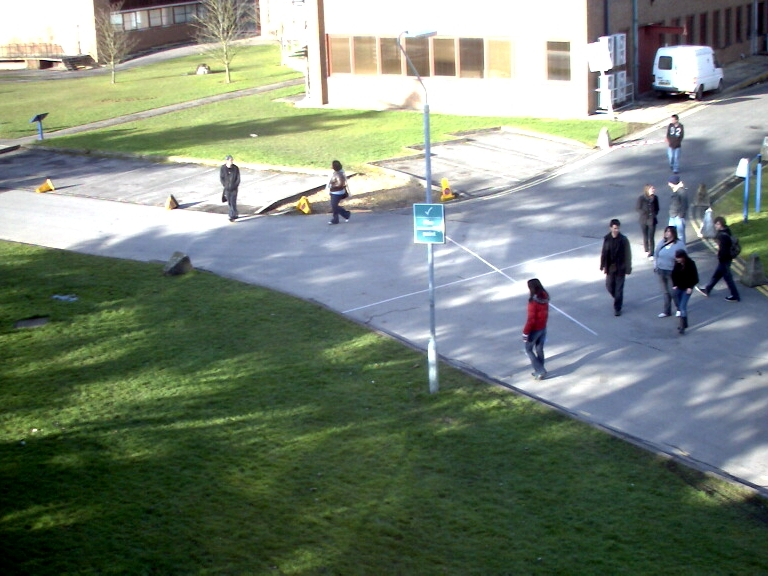
\includegraphics{PETS2009Example.jpg}

Abb. 1: Verwendetes Bild des PETS2009-Benchmarkdatensatzes

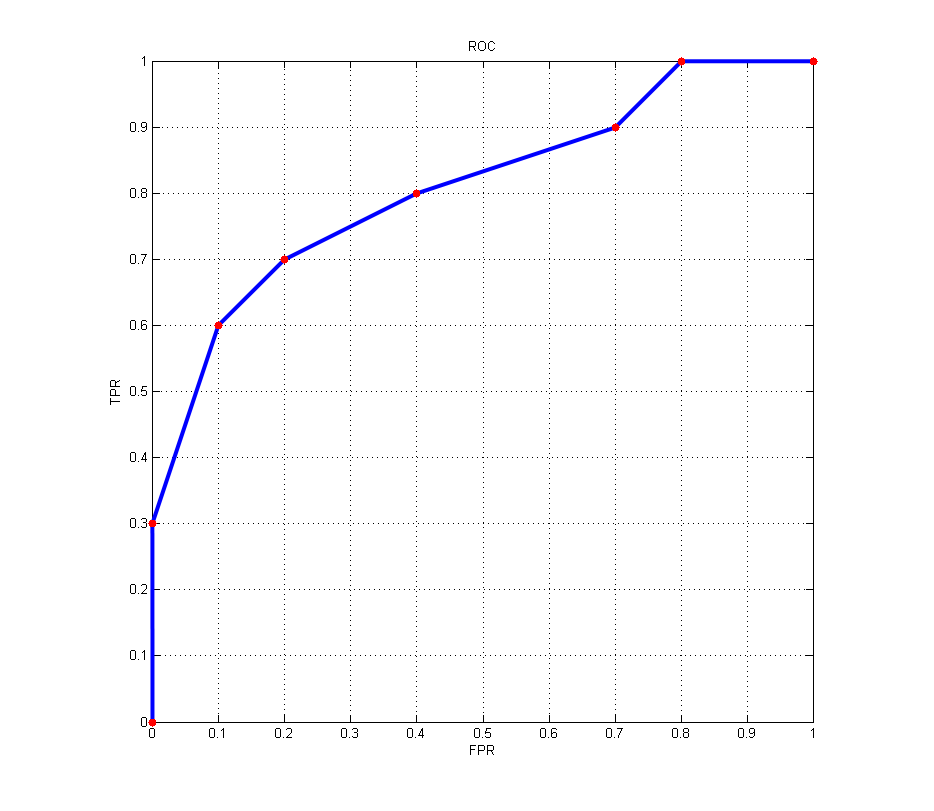
\includegraphics{ROC-Curve.png}

Abb. 2: ROC-Kurve

\begin{itemize}
\tightlist
\item
  Lesen Sie aus diesem Diagramm für die rot markierten Punkte die True
  Positive Rate und die False Positive Rate ab (In der Reihenfolge von
  (0, 0) bis (1, 1); alle Werte besitzen nur eine Nachkommastelle).
\item
  Übertragen Sie das ROC-Diagramm in ein Precision-Recall-Diagramm
  (Ermitteln Sie P anhand Abb. 1).
\item
  Hinweis: Der Wert der Precision für den Punkt (0, 0) der ROC-Kurve
  kann nicht berechnet werden (die Berechnung ergibt NaN). Setzen sie
  statt dessen den Grenzwert ein, der an der Stelle Recall=0 für die
  Precision einen Wert von 1 annimmt.
\item
  Berechnen Sie den bestmöglichen \(F_1\)-Score und die beste Balanced
  Error Rate, die dieser Personendetektor erreichen kann, wenn für das
  jeweilige Performance-Maß der am besten geeignete der acht
  Schwellwerte (rote Punkte) gewählt wird.
\end{itemize}

Ihre Lösung:

    \begin{Verbatim}[commandchars=\\\{\}]
{\color{incolor}In [{\color{incolor} }]:} \PY{o}{\PYZpc{}}\PY{k}{matplotlib} inline
        
        \PY{k+kn}{import} \PY{n+nn}{numpy}
        \PY{k+kn}{import} \PY{n+nn}{matplotlib}\PY{n+nn}{.}\PY{n+nn}{pyplot} \PY{k}{as} \PY{n+nn}{plot}
        
        \PY{c+c1}{\PYZsh{} Hilfsfunktion zum Zeichnen der Lösung}
        \PY{k}{def} \PY{n+nf}{plot\PYZus{}ROC}\PY{p}{(}\PY{n}{TPR}\PY{p}{,} \PY{n}{FPR}\PY{p}{,} \PY{n}{BER}\PY{o}{=}\PY{k+kc}{None}\PY{p}{)}\PY{p}{:}
            \PY{l+s+sd}{\PYZdq{}\PYZdq{}\PYZdq{}ROC\PYZhy{}Kurve zeichnen\PYZdq{}\PYZdq{}\PYZdq{}}
            \PY{k}{if} \PY{n}{BER} \PY{o}{!=} \PY{k+kc}{None}\PY{p}{:}
                \PY{n}{f} \PY{o}{=} \PY{n}{numpy}\PY{o}{.}\PY{n}{linspace}\PY{p}{(}\PY{l+m+mf}{0.0}\PY{p}{,} \PY{l+m+mf}{1.0}\PY{p}{,} \PY{l+m+mi}{500}\PY{p}{)}
                \PY{n}{t} \PY{o}{=} \PY{n}{numpy}\PY{o}{.}\PY{n}{linspace}\PY{p}{(}\PY{l+m+mf}{0.0}\PY{p}{,} \PY{l+m+mf}{1.0}\PY{p}{,} \PY{l+m+mi}{500}\PY{p}{)}
                \PY{n}{fpr}\PY{p}{,} \PY{n}{tpr} \PY{o}{=} \PY{n}{numpy}\PY{o}{.}\PY{n}{meshgrid}\PY{p}{(}\PY{n}{f}\PY{p}{,} \PY{n}{t}\PY{p}{)}
                \PY{n}{balanced\PYZus{}error\PYZus{}rate} \PY{o}{=} \PY{l+m+mf}{0.5} \PY{o}{*} \PY{p}{(}\PY{n}{fpr} \PY{o}{+} \PY{p}{(}\PY{l+m+mi}{1} \PY{o}{\PYZhy{}} \PY{n}{tpr}\PY{p}{)}\PY{p}{)}
                \PY{n}{plot}\PY{o}{.}\PY{n}{contour}\PY{p}{(}\PY{n}{f}\PY{p}{,} \PY{n}{t}\PY{p}{,} \PY{n}{balanced\PYZus{}error\PYZus{}rate}\PY{p}{,} \PY{n}{levels}\PY{o}{=}\PY{p}{[}\PY{n}{BER}\PY{p}{]}\PY{p}{,}
                             \PY{n}{linewidths}\PY{o}{=}\PY{l+m+mi}{2}\PY{p}{,} \PY{n}{colors}\PY{o}{=}\PY{l+s+s1}{\PYZsq{}}\PY{l+s+s1}{g}\PY{l+s+s1}{\PYZsq{}}\PY{p}{)}
                \PY{n}{plot}\PY{o}{.}\PY{n}{title}\PY{p}{(}\PY{l+s+s1}{\PYZsq{}}\PY{l+s+s1}{ROC, Balanced Error Rate}\PY{l+s+s1}{\PYZsq{}}\PY{p}{)}
                \PY{n}{marker} \PY{o}{=} \PY{l+s+s1}{\PYZsq{}}\PY{l+s+s1}{:}\PY{l+s+s1}{\PYZsq{}}
            \PY{k}{else}\PY{p}{:}
                \PY{n}{plot}\PY{o}{.}\PY{n}{title}\PY{p}{(}\PY{l+s+s1}{\PYZsq{}}\PY{l+s+s1}{ROC}\PY{l+s+s1}{\PYZsq{}}\PY{p}{)}
                \PY{n}{marker} \PY{o}{=} \PY{l+s+s1}{\PYZsq{}}\PY{l+s+s1}{\PYZhy{}}\PY{l+s+s1}{\PYZsq{}}
                
            \PY{n}{plot}\PY{o}{.}\PY{n}{plot}\PY{p}{(}\PY{n}{FPR}\PY{p}{,} \PY{n}{TPR}\PY{p}{,} \PY{l+s+s1}{\PYZsq{}}\PY{l+s+s1}{b}\PY{l+s+s1}{\PYZsq{}}\PY{o}{+}\PY{n}{marker}\PY{p}{,} \PY{n}{linewidth}\PY{o}{=}\PY{l+m+mi}{2}\PY{p}{)}
            \PY{n}{plot}\PY{o}{.}\PY{n}{plot}\PY{p}{(}\PY{n}{FPR}\PY{p}{,} \PY{n}{TPR}\PY{p}{,} \PY{l+s+s1}{\PYZsq{}}\PY{l+s+s1}{r.}\PY{l+s+s1}{\PYZsq{}}\PY{p}{,} \PY{n}{markersize}\PY{o}{=}\PY{l+m+mi}{20}\PY{p}{)}
            \PY{n}{plot}\PY{o}{.}\PY{n}{axis}\PY{p}{(}\PY{l+s+s1}{\PYZsq{}}\PY{l+s+s1}{equal}\PY{l+s+s1}{\PYZsq{}}\PY{p}{)}
            \PY{n}{plot}\PY{o}{.}\PY{n}{axis}\PY{p}{(}\PY{p}{[}\PY{l+m+mi}{0}\PY{p}{,} \PY{l+m+mi}{1}\PY{p}{,} \PY{l+m+mi}{0}\PY{p}{,} \PY{l+m+mi}{1}\PY{p}{]}\PY{p}{)}
            \PY{n}{plot}\PY{o}{.}\PY{n}{xlabel}\PY{p}{(}\PY{l+s+s1}{\PYZsq{}}\PY{l+s+s1}{FPR}\PY{l+s+s1}{\PYZsq{}}\PY{p}{)}
            \PY{n}{plot}\PY{o}{.}\PY{n}{ylabel}\PY{p}{(}\PY{l+s+s1}{\PYZsq{}}\PY{l+s+s1}{TPR}\PY{l+s+s1}{\PYZsq{}}\PY{p}{)}
            \PY{n}{plot}\PY{o}{.}\PY{n}{grid}\PY{p}{(}\PY{l+s+s1}{\PYZsq{}}\PY{l+s+s1}{on}\PY{l+s+s1}{\PYZsq{}}\PY{p}{)}
            \PY{n}{plot}\PY{o}{.}\PY{n}{show}\PY{p}{(}\PY{p}{)}
            
        \PY{c+c1}{\PYZsh{} Hilfsfunktion zum Zeichnen der Lösung}
        \PY{k}{def} \PY{n+nf}{plot\PYZus{}PR}\PY{p}{(}\PY{n}{Precision}\PY{p}{,} \PY{n}{Recall}\PY{p}{,} \PY{n}{F\PYZus{}1}\PY{o}{=}\PY{k+kc}{None}\PY{p}{)}\PY{p}{:}
            \PY{l+s+sd}{\PYZdq{}\PYZdq{}\PYZdq{}Precision\PYZhy{}Recall\PYZhy{}Kurve zeichnen\PYZdq{}\PYZdq{}\PYZdq{}}
            \PY{k}{if} \PY{n}{F\PYZus{}1} \PY{o}{!=} \PY{k+kc}{None}\PY{p}{:}
                \PY{n}{p} \PY{o}{=} \PY{n}{numpy}\PY{o}{.}\PY{n}{linspace}\PY{p}{(}\PY{l+m+mf}{0.0}\PY{p}{,} \PY{l+m+mf}{1.0}\PY{p}{,} \PY{l+m+mi}{500}\PY{p}{)}
                \PY{n}{r} \PY{o}{=} \PY{n}{numpy}\PY{o}{.}\PY{n}{linspace}\PY{p}{(}\PY{l+m+mf}{0.0}\PY{p}{,} \PY{l+m+mf}{1.0}\PY{p}{,} \PY{l+m+mi}{500}\PY{p}{)}
                \PY{n}{prec}\PY{p}{,} \PY{n}{rec} \PY{o}{=} \PY{n}{numpy}\PY{o}{.}\PY{n}{meshgrid}\PY{p}{(}\PY{n}{p}\PY{p}{,} \PY{n}{r}\PY{p}{)}
                \PY{n}{F\PYZus{}1\PYZus{}score} \PY{o}{=} \PY{l+m+mf}{2.0} \PY{o}{*} \PY{n}{numpy}\PY{o}{.}\PY{n}{divide}\PY{p}{(}\PY{n}{numpy}\PY{o}{.}\PY{n}{multiply}\PY{p}{(}\PY{n}{prec}\PY{p}{,} \PY{n}{rec}\PY{p}{)}\PY{p}{,} \PY{n}{prec} \PY{o}{+} \PY{n}{rec} \PY{o}{+} \PY{l+m+mf}{1e\PYZhy{}12}\PY{p}{)}
                \PY{n}{plot}\PY{o}{.}\PY{n}{contour}\PY{p}{(}\PY{n}{p}\PY{p}{,} \PY{n}{r}\PY{p}{,} \PY{n}{F\PYZus{}1\PYZus{}score}\PY{p}{,} \PY{n}{levels}\PY{o}{=}\PY{p}{[}\PY{n}{F\PYZus{}1}\PY{p}{]}\PY{p}{,} \PY{n}{linewidths}\PY{o}{=}\PY{l+m+mi}{2}\PY{p}{,} \PY{n}{colors}\PY{o}{=}\PY{l+s+s1}{\PYZsq{}}\PY{l+s+s1}{g}\PY{l+s+s1}{\PYZsq{}}\PY{p}{)}
                \PY{n}{plot}\PY{o}{.}\PY{n}{title}\PY{p}{(}\PY{l+s+s1}{\PYZsq{}}\PY{l+s+s1}{Precision\PYZhy{}Recall, \PYZdl{}F\PYZus{}1\PYZdl{}\PYZhy{}Score}\PY{l+s+s1}{\PYZsq{}}\PY{p}{)}
                \PY{n}{marker} \PY{o}{=} \PY{l+s+s1}{\PYZsq{}}\PY{l+s+s1}{:}\PY{l+s+s1}{\PYZsq{}}
            \PY{k}{else}\PY{p}{:}
                \PY{n}{plot}\PY{o}{.}\PY{n}{title}\PY{p}{(}\PY{l+s+s1}{\PYZsq{}}\PY{l+s+s1}{Precision\PYZhy{}Recall}\PY{l+s+s1}{\PYZsq{}}\PY{p}{)}
                \PY{n}{marker} \PY{o}{=} \PY{l+s+s1}{\PYZsq{}}\PY{l+s+s1}{\PYZhy{}}\PY{l+s+s1}{\PYZsq{}}
            
            \PY{n}{plot}\PY{o}{.}\PY{n}{plot}\PY{p}{(}\PY{n}{Recall}\PY{p}{,} \PY{n}{Precision}\PY{p}{,} \PY{l+s+s1}{\PYZsq{}}\PY{l+s+s1}{b}\PY{l+s+s1}{\PYZsq{}}\PY{o}{+}\PY{n}{marker}\PY{p}{,} \PY{n}{linewidth}\PY{o}{=}\PY{l+m+mi}{2}\PY{p}{)}
            \PY{n}{plot}\PY{o}{.}\PY{n}{plot}\PY{p}{(}\PY{n}{Recall}\PY{p}{,} \PY{n}{Precision}\PY{p}{,} \PY{l+s+s1}{\PYZsq{}}\PY{l+s+s1}{r.}\PY{l+s+s1}{\PYZsq{}}\PY{p}{,} \PY{n}{markersize}\PY{o}{=}\PY{l+m+mi}{20}\PY{p}{)}
            \PY{n}{plot}\PY{o}{.}\PY{n}{axis}\PY{p}{(}\PY{l+s+s1}{\PYZsq{}}\PY{l+s+s1}{equal}\PY{l+s+s1}{\PYZsq{}}\PY{p}{)}
            \PY{n}{plot}\PY{o}{.}\PY{n}{axis}\PY{p}{(}\PY{p}{[}\PY{l+m+mi}{0}\PY{p}{,} \PY{l+m+mi}{1}\PY{p}{,} \PY{l+m+mi}{0}\PY{p}{,} \PY{l+m+mi}{1}\PY{p}{]}\PY{p}{)}
            \PY{n}{plot}\PY{o}{.}\PY{n}{xlabel}\PY{p}{(}\PY{l+s+s1}{\PYZsq{}}\PY{l+s+s1}{Recall}\PY{l+s+s1}{\PYZsq{}}\PY{p}{)}
            \PY{n}{plot}\PY{o}{.}\PY{n}{ylabel}\PY{p}{(}\PY{l+s+s1}{\PYZsq{}}\PY{l+s+s1}{Precision}\PY{l+s+s1}{\PYZsq{}}\PY{p}{)}
            \PY{n}{plot}\PY{o}{.}\PY{n}{grid}\PY{p}{(}\PY{l+s+s1}{\PYZsq{}}\PY{l+s+s1}{on}\PY{l+s+s1}{\PYZsq{}}\PY{p}{)}
            \PY{n}{plot}\PY{o}{.}\PY{n}{show}\PY{p}{(}\PY{p}{)}
        
        
        
        
        \PY{c+c1}{\PYZsh{} Zahlen ersetzen durch Ihre berechneten Werte}
        \PY{n}{true\PYZus{}positive\PYZus{}rate}  \PY{o}{=} \PY{p}{[}\PY{l+m+mf}{0.0}\PY{p}{,} \PY{l+m+mf}{0.0}\PY{p}{,} \PY{l+m+mf}{0.0}\PY{p}{,} \PY{l+m+mf}{0.0}\PY{p}{,} \PY{l+m+mf}{0.0}\PY{p}{,} \PY{l+m+mf}{0.0}\PY{p}{,} \PY{l+m+mf}{0.0}\PY{p}{,} \PY{l+m+mf}{0.0}\PY{p}{]}
        \PY{n}{false\PYZus{}positive\PYZus{}rate} \PY{o}{=} \PY{p}{[}\PY{l+m+mf}{0.0}\PY{p}{,} \PY{l+m+mf}{0.0}\PY{p}{,} \PY{l+m+mf}{0.0}\PY{p}{,} \PY{l+m+mf}{0.0}\PY{p}{,} \PY{l+m+mf}{0.0}\PY{p}{,} \PY{l+m+mf}{0.0}\PY{p}{,} \PY{l+m+mf}{0.0}\PY{p}{,} \PY{l+m+mf}{0.0}\PY{p}{]}
        \PY{n}{precision}           \PY{o}{=} \PY{p}{[}\PY{l+m+mf}{0.0}\PY{p}{,} \PY{l+m+mf}{0.0}\PY{p}{,} \PY{l+m+mf}{0.0}\PY{p}{,} \PY{l+m+mf}{0.0}\PY{p}{,} \PY{l+m+mf}{0.0}\PY{p}{,} \PY{l+m+mf}{0.0}\PY{p}{,} \PY{l+m+mf}{0.0}\PY{p}{,} \PY{l+m+mf}{0.0}\PY{p}{]}
        \PY{n}{recall}              \PY{o}{=} \PY{p}{[}\PY{l+m+mf}{0.0}\PY{p}{,} \PY{l+m+mf}{0.0}\PY{p}{,} \PY{l+m+mf}{0.0}\PY{p}{,} \PY{l+m+mf}{0.0}\PY{p}{,} \PY{l+m+mf}{0.0}\PY{p}{,} \PY{l+m+mf}{0.0}\PY{p}{,} \PY{l+m+mf}{0.0}\PY{p}{,} \PY{l+m+mf}{0.0}\PY{p}{]}
        \PY{n}{bester\PYZus{}f\PYZus{}1\PYZus{}score} \PY{o}{=} \PY{l+m+mf}{0.00}
        \PY{n}{beste\PYZus{}balanced\PYZus{}error\PYZus{}rate} \PY{o}{=} \PY{l+m+mf}{0.00}
        
        
        
        
        \PY{c+c1}{\PYZsh{} Visualisierung der Lösung}
        \PY{n}{plot\PYZus{}ROC}\PY{p}{(}\PY{n}{true\PYZus{}positive\PYZus{}rate}\PY{p}{,} \PY{n}{false\PYZus{}positive\PYZus{}rate}\PY{p}{,} \PY{n}{beste\PYZus{}balanced\PYZus{}error\PYZus{}rate}\PY{p}{)}
        \PY{n}{plot\PYZus{}PR}\PY{p}{(}\PY{n}{precision}\PY{p}{,} \PY{n}{recall}\PY{p}{,} \PY{n}{bester\PYZus{}f\PYZus{}1\PYZus{}score}\PY{p}{)}
        
        \PY{c+c1}{\PYZsh{} Ergebnisse überprüfen}
        \PY{k+kn}{import} \PY{n+nn}{test\PYZus{}z\PYZus{}ip}
        \PY{n}{result} \PY{o}{=} \PY{n}{numpy}\PY{o}{.}\PY{n}{matrix}\PY{p}{(}\PY{n}{true\PYZus{}positive\PYZus{}rate} \PY{o}{+} \PY{n}{false\PYZus{}positive\PYZus{}rate} \PY{o}{+} \PYZbs{}
                              \PY{n}{precision} \PY{o}{+} \PY{n}{recall} \PY{o}{+} \PYZbs{}
                              \PY{p}{[}\PY{n}{bester\PYZus{}f\PYZus{}1\PYZus{}score}\PY{p}{,} \PY{n}{beste\PYZus{}balanced\PYZus{}error\PYZus{}rate}\PY{p}{]}\PY{p}{)}
        \PY{n}{test\PYZus{}z\PYZus{}ip}\PY{o}{.}\PY{n}{loesung\PYZus{}z7}\PY{p}{(}\PY{n}{result}\PY{p}{)}
\end{Verbatim}


    Bonus: 1\%,\(\;\;\;\)Frist: 14 Tage nach Bearbeitung von Übungsaufgabe
23, 12:00 Uhr

\subsubsection{Zusatzaufgabe 8}\label{zusatzaufgabe-8}

Um Gesichter in Bildern zu erkennen soll ein kaskadierter
AdaBoost-Detektor trainiert werden. Trainieren Sie exemplarisch den
Strong Learner für die erste Kaskadenstufe.

Das Ziel der ersten Kaskadenstufe ist es Nicht-Gesichter mit möglichst
wenig Rechenaufwand zu erkennen und sie für die weiteren Kaskadenstufen
zu entfernen. Daher sollen in dieser Kaskadenstufe nur die zwei am
besten geeigneten Merkmale verwendet werden. Im Trainingsdatensatz sind
10 Gesichter und 40 andere Objekte enthalten. Die Filterantwort der
beiden Merkmale für die 50 Trainingsbeispiele ist in Abb. 3 dargestellt.
Es entsteht ein 2-dimensionaler Merkmalsraum.

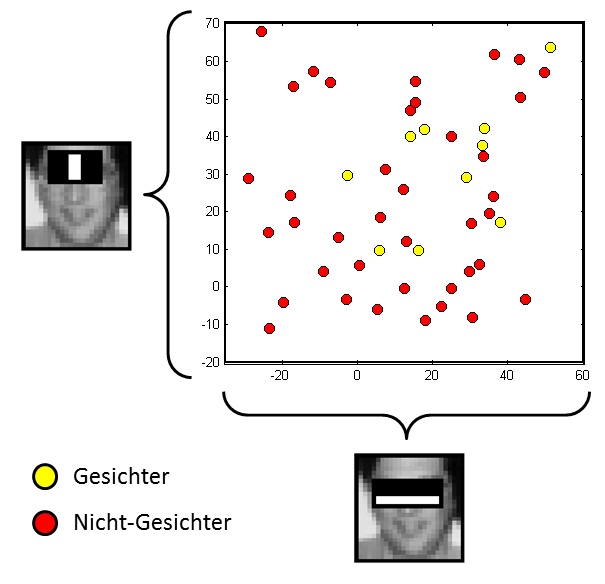
\includegraphics{AdaBoost.png}

Abb. 3: Trainingsbeispiele

Verwenden Sie den AdaBoost-Algorithmus aus der Vorlesung um mehrere Weak
Learner, die jeweils nur auf einem der beiden Merkmale arbeiten, zu
einem Strong Learner zusammenzufügen. Stellen Sie den Schwellwert T des
Strong Learners für die Mehrheitsentscheidung so ein, dass eine True
Positive Rate von 1.0 erreicht wird, d.h. dass alle Gesichter auch als
Gesichter erkannt werden

Vorgehensweise: - Berechnen Sie die Outputs des Strong Learners für alle
Gesichter und verwenden sie das Minimum als Schwellwert T, d.h. vergeben
Sie das Klassenlabel 1 falls der Output des Strong Learners
\textgreater{}= T ist, und 0 sonst.

Fügen Sie so lange weitere Weak Learner hinzu bis die False Positive
Rate des Strong Learners bei dem zuvor berechneten Schwellwert T kleiner
oder gleich 0.4 ist. Wählen Sie in jeder Iteration den Weak Learner aus,
der den kleinsten Fehler verursacht. Den am besten geeigneten
Schwellwert entlang einer Dimension unter Berücksichtigung der aktuellen
Gewichte liefert die Funktion get\_weak\_learner\_schwellwert: - z.B.
\(\texttt{t0 = get_weak_learner_schwellwert(x[0], label, d)}\) für die
Dimension 0 (bzw. Merkmal 0).

Vorgehensweise: - Berechnen Sie die Schwellwerte für die beiden
Dimensionen. - Ermitteln Sie den gewichteten Fehler epsilon für beide
Weak Learner. - Fügen Sie nur den Weak Learner zum Strong Learner hinzu,
der den geringeren gewichteten Fehler verursacht.

Hinweis: Es ist üblich, dass ein Weak Lerner in späteren Iterationen
erneut ausgewählt wird. Es ist auch normal, dass mehrere ausgewählte
Weak Learner den gleichen Schwellwert verwenden.

Die Gewichte d sollen für alle Datenpunkte mit dem gleichen Wert (1/N)
initialisiert werden.

Um die Gewichte und die ausgewählten Weak Learner zu visualisieren
können Sie die Funktion plot\_input\_and\_weights benutzen: - z.B.
\(\texttt{plot_daten_and_gewichte(x, label, d, weak_learner_dimension, weak_learner_schwellwert)}\)
- weak\_learner\_dimension ... Liste der ausgewählten Dimensionen
(jeweils 0 oder 1) - weak\_learner\_schwellwert ... Liste zugehöriger
Thresholds der jeweiligen Weak Learner

gegeben \(\&\) Hilfsfunktionen

    \begin{Verbatim}[commandchars=\\\{\}]
{\color{incolor}In [{\color{incolor} }]:} \PY{o}{\PYZpc{}}\PY{k}{matplotlib} inline
        
        \PY{k+kn}{import} \PY{n+nn}{numpy}
        \PY{k+kn}{import} \PY{n+nn}{math}
        \PY{k+kn}{import} \PY{n+nn}{matplotlib}\PY{n+nn}{.}\PY{n+nn}{pyplot} \PY{k}{as} \PY{n+nn}{plot}
        
        \PY{c+c1}{\PYZsh{} gegeben}
        \PY{n}{x\PYZus{}face}     \PY{o}{=} \PY{n}{numpy}\PY{o}{.}\PY{n}{matrix}\PY{p}{(}\PY{p}{[}\PY{p}{[}  \PY{l+m+mf}{5.93}\PY{p}{,}  \PY{l+m+mf}{33.85}\PY{p}{,}  \PY{l+m+mf}{14.15}\PY{p}{,}  \PY{l+m+mf}{51.22}\PY{p}{,}  \PY{l+m+mf}{17.92}\PY{p}{,}
                                     \PY{l+m+mf}{37.93}\PY{p}{,}  \PY{l+m+mf}{33.28}\PY{p}{,}  \PY{l+m+mf}{16.17}\PY{p}{,}  \PY{o}{\PYZhy{}}\PY{l+m+mf}{2.56}\PY{p}{,}  \PY{l+m+mf}{29.11} \PY{p}{]}\PY{p}{,}
                                   \PY{p}{[}  \PY{l+m+mf}{9.78}\PY{p}{,}  \PY{l+m+mf}{42.28}\PY{p}{,}  \PY{l+m+mf}{40.15}\PY{p}{,}  \PY{l+m+mf}{63.84}\PY{p}{,}  \PY{l+m+mf}{41.82}\PY{p}{,}
                                     \PY{l+m+mf}{17.12}\PY{p}{,}  \PY{l+m+mf}{37.60}\PY{p}{,}   \PY{l+m+mf}{9.81}\PY{p}{,}  \PY{l+m+mf}{29.60}\PY{p}{,}  \PY{l+m+mf}{29.03} \PY{p}{]}\PY{p}{]}\PY{p}{)}
        
        \PY{n}{x\PYZus{}non\PYZus{}face} \PY{o}{=} \PY{n}{numpy}\PY{o}{.}\PY{n}{matrix}\PY{p}{(}\PY{p}{[}\PY{p}{[} \PY{l+m+mf}{20.00}\PY{p}{,}  \PY{l+m+mf}{36.46}\PY{p}{,}  \PY{l+m+mf}{25.00}\PY{p}{,}  \PY{l+m+mf}{13.97}\PY{p}{,}  \PY{l+m+mf}{43.37}\PY{p}{,}
                                     \PY{o}{\PYZhy{}}\PY{l+m+mf}{7.13}\PY{p}{,}  \PY{l+m+mf}{30.57}\PY{p}{,}  \PY{l+m+mf}{30.29}\PY{p}{,}   \PY{l+m+mf}{0.43}\PY{p}{,}  \PY{l+m+mf}{15.42}\PY{p}{,}
                                     \PY{l+m+mf}{35.00}\PY{p}{,} \PY{o}{\PYZhy{}}\PY{l+m+mf}{25.68}\PY{p}{,}  \PY{l+m+mf}{12.46}\PY{p}{,}  \PY{l+m+mf}{32.33}\PY{p}{,}  \PY{l+m+mf}{44.72}\PY{p}{,}
                                    \PY{o}{\PYZhy{}}\PY{l+m+mf}{19.60}\PY{p}{,}  \PY{l+m+mf}{15.50}\PY{p}{,}   \PY{l+m+mf}{7.55}\PY{p}{,} \PY{o}{\PYZhy{}}\PY{l+m+mf}{29.04}\PY{p}{,}  \PY{o}{\PYZhy{}}\PY{l+m+mf}{3.03}\PY{p}{,}
                                    \PY{o}{\PYZhy{}}\PY{l+m+mf}{17.02}\PY{p}{,}  \PY{l+m+mf}{33.54}\PY{p}{,}  \PY{o}{\PYZhy{}}\PY{l+m+mf}{5.10}\PY{p}{,}  \PY{l+m+mf}{12.28}\PY{p}{,} \PY{o}{\PYZhy{}}\PY{l+m+mf}{16.74}\PY{p}{,}
                                     \PY{l+m+mf}{18.15}\PY{p}{,}  \PY{o}{\PYZhy{}}\PY{l+m+mf}{8.96}\PY{p}{,}  \PY{l+m+mf}{22.32}\PY{p}{,}  \PY{l+m+mf}{25.13}\PY{p}{,}  \PY{l+m+mf}{29.85}\PY{p}{,}
                                      \PY{l+m+mf}{6.04}\PY{p}{,} \PY{o}{\PYZhy{}}\PY{l+m+mf}{23.29}\PY{p}{,} \PY{o}{\PYZhy{}}\PY{l+m+mf}{11.68}\PY{p}{,}  \PY{l+m+mf}{43.06}\PY{p}{,} \PY{o}{\PYZhy{}}\PY{l+m+mf}{17.80}\PY{p}{,}
                                     \PY{l+m+mf}{36.06}\PY{p}{,}  \PY{l+m+mf}{13.06}\PY{p}{,}  \PY{l+m+mf}{49.69}\PY{p}{,} \PY{o}{\PYZhy{}}\PY{l+m+mf}{23.74}\PY{p}{,}   \PY{l+m+mf}{5.41} \PY{p}{]}\PY{p}{,}
                                   \PY{p}{[}\PY{o}{\PYZhy{}}\PY{l+m+mf}{23.93}\PY{p}{,}  \PY{l+m+mf}{61.95}\PY{p}{,}  \PY{l+m+mf}{40.00}\PY{p}{,}  \PY{l+m+mf}{46.99}\PY{p}{,}  \PY{l+m+mf}{50.38}\PY{p}{,}
                                     \PY{l+m+mf}{54.49}\PY{p}{,}  \PY{o}{\PYZhy{}}\PY{l+m+mf}{8.24}\PY{p}{,}  \PY{l+m+mf}{16.98}\PY{p}{,}   \PY{l+m+mf}{5.78}\PY{p}{,}  \PY{l+m+mf}{49.00}\PY{p}{,}
                                     \PY{l+m+mf}{19.51}\PY{p}{,}  \PY{l+m+mf}{67.85}\PY{p}{,}  \PY{o}{\PYZhy{}}\PY{l+m+mf}{0.45}\PY{p}{,}   \PY{l+m+mf}{6.10}\PY{p}{,}  \PY{o}{\PYZhy{}}\PY{l+m+mf}{3.35}\PY{p}{,}
                                     \PY{o}{\PYZhy{}}\PY{l+m+mf}{4.11}\PY{p}{,}  \PY{l+m+mf}{54.54}\PY{p}{,}  \PY{l+m+mf}{31.37}\PY{p}{,}  \PY{l+m+mf}{28.98}\PY{p}{,}  \PY{o}{\PYZhy{}}\PY{l+m+mf}{3.40}\PY{p}{,}
                                     \PY{l+m+mf}{53.24}\PY{p}{,}  \PY{l+m+mf}{34.76}\PY{p}{,}  \PY{l+m+mf}{13.07}\PY{p}{,}  \PY{l+m+mf}{26.06}\PY{p}{,}  \PY{l+m+mf}{17.14}\PY{p}{,}
                                     \PY{o}{\PYZhy{}}\PY{l+m+mf}{8.92}\PY{p}{,}   \PY{l+m+mf}{4.19}\PY{p}{,}  \PY{o}{\PYZhy{}}\PY{l+m+mf}{5.13}\PY{p}{,}  \PY{o}{\PYZhy{}}\PY{l+m+mf}{0.28}\PY{p}{,}   \PY{l+m+mf}{4.19}\PY{p}{,}
                                     \PY{l+m+mf}{18.38}\PY{p}{,} \PY{o}{\PYZhy{}}\PY{l+m+mf}{11.02}\PY{p}{,}  \PY{l+m+mf}{57.21}\PY{p}{,}  \PY{l+m+mf}{60.58}\PY{p}{,}  \PY{l+m+mf}{24.26}\PY{p}{,}
                                     \PY{l+m+mf}{24.14}\PY{p}{,}  \PY{l+m+mf}{12.01}\PY{p}{,}  \PY{l+m+mf}{57.00}\PY{p}{,}  \PY{l+m+mf}{14.53}\PY{p}{,}  \PY{o}{\PYZhy{}}\PY{l+m+mf}{6.10} \PY{p}{]}\PY{p}{]}\PY{p}{)}
        
        \PY{n}{x} \PY{o}{=} \PY{n}{numpy}\PY{o}{.}\PY{n}{concatenate}\PY{p}{(}\PY{p}{(}\PY{n}{x\PYZus{}face}\PY{p}{,} \PY{n}{x\PYZus{}non\PYZus{}face}\PY{p}{)}\PY{p}{,} \PY{n}{axis}\PY{o}{=}\PY{l+m+mi}{1}\PY{p}{)}
        
        \PY{c+c1}{\PYZsh{} Legende (Label): 1 = Gesicht, 0 = Nicht\PYZhy{}Gesicht}
        \PY{n}{label} \PY{o}{=} \PY{n}{numpy}\PY{o}{.}\PY{n}{concatenate}\PY{p}{(}\PY{p}{(}\PY{n}{numpy}\PY{o}{.}\PY{n}{ones}\PY{p}{(}\PY{l+m+mi}{10}\PY{p}{)}\PY{p}{,} \PY{n}{numpy}\PY{o}{.}\PY{n}{zeros}\PY{p}{(}\PY{l+m+mi}{40}\PY{p}{)}\PY{p}{)}\PY{p}{)}
        
        \PY{c+c1}{\PYZsh{} Anzahl Datenpunkte}
        \PY{n}{N} \PY{o}{=} \PY{n}{x}\PY{o}{.}\PY{n}{shape}\PY{p}{[}\PY{l+m+mi}{1}\PY{p}{]}
        
        \PY{c+c1}{\PYZsh{} initiale Gewichte}
        \PY{n}{d} \PY{o}{=} \PY{n}{numpy}\PY{o}{.}\PY{n}{ones}\PY{p}{(}\PY{n}{N}\PY{p}{)} \PY{o}{/} \PY{n+nb}{float}\PY{p}{(}\PY{n}{N}\PY{p}{)}
        
        \PY{c+c1}{\PYZsh{} Hilfsfuntionen}
        \PY{k}{def} \PY{n+nf}{plot\PYZus{}daten\PYZus{}and\PYZus{}gewichte}\PY{p}{(}\PY{n}{x}\PY{p}{,} \PY{n}{label}\PY{p}{,} \PY{n}{d}\PY{o}{=}\PY{k+kc}{None}\PY{p}{,} \PY{n}{weak\PYZus{}learner\PYZus{}dimension}\PY{o}{=}\PY{k+kc}{None}\PY{p}{,}
                                    \PY{n}{weak\PYZus{}learner\PYZus{}schwellwert}\PY{o}{=}\PY{k+kc}{None}\PY{p}{)}\PY{p}{:}
            \PY{n}{N} \PY{o}{=} \PY{n}{x}\PY{o}{.}\PY{n}{shape}\PY{p}{[}\PY{l+m+mi}{1}\PY{p}{]}
            
            \PY{k}{if} \PY{n}{d} \PY{o}{==} \PY{k+kc}{None}\PY{p}{:}
                \PY{n}{d} \PY{o}{=} \PY{n}{numpy}\PY{o}{.}\PY{n}{ones}\PY{p}{(}\PY{n}{N}\PY{p}{)} \PY{o}{/} \PY{n+nb}{float}\PY{p}{(}\PY{n}{N}\PY{p}{)}
                
            \PY{n}{max\PYZus{}circle\PYZus{}radius} \PY{o}{=} \PY{l+m+mi}{60}
            
            \PY{c+c1}{\PYZsh{} Visualisiere Problemstellung}
            \PY{n}{plot}\PY{o}{.}\PY{n}{plot}\PY{p}{(}\PY{p}{[}\PY{o}{\PYZhy{}}\PY{l+m+mi}{35}\PY{p}{,} \PY{l+m+mi}{60}\PY{p}{]}\PY{p}{,} \PY{p}{[}\PY{o}{\PYZhy{}}\PY{l+m+mi}{20}\PY{p}{,} \PY{o}{\PYZhy{}}\PY{l+m+mi}{20}\PY{p}{]}\PY{p}{,} \PY{l+s+s1}{\PYZsq{}}\PY{l+s+s1}{k\PYZhy{}}\PY{l+s+s1}{\PYZsq{}}\PY{p}{,} \PY{n}{linewidth}\PY{o}{=}\PY{l+m+mi}{2}\PY{p}{)}
            \PY{n}{plot}\PY{o}{.}\PY{n}{plot}\PY{p}{(}\PY{p}{[}\PY{o}{\PYZhy{}}\PY{l+m+mi}{35}\PY{p}{,} \PY{l+m+mi}{60}\PY{p}{]}\PY{p}{,} \PY{p}{[}\PY{l+m+mi}{70}\PY{p}{,} \PY{l+m+mi}{70}\PY{p}{]}\PY{p}{,} \PY{l+s+s1}{\PYZsq{}}\PY{l+s+s1}{k\PYZhy{}}\PY{l+s+s1}{\PYZsq{}}\PY{p}{,} \PY{n}{linewidth}\PY{o}{=}\PY{l+m+mi}{2}\PY{p}{)}
            \PY{n}{plot}\PY{o}{.}\PY{n}{plot}\PY{p}{(}\PY{p}{[}\PY{o}{\PYZhy{}}\PY{l+m+mi}{35}\PY{p}{,} \PY{o}{\PYZhy{}}\PY{l+m+mi}{35}\PY{p}{]}\PY{p}{,} \PY{p}{[}\PY{o}{\PYZhy{}}\PY{l+m+mi}{20}\PY{p}{,} \PY{l+m+mi}{70}\PY{p}{]}\PY{p}{,} \PY{l+s+s1}{\PYZsq{}}\PY{l+s+s1}{k\PYZhy{}}\PY{l+s+s1}{\PYZsq{}}\PY{p}{,} \PY{n}{linewidth}\PY{o}{=}\PY{l+m+mi}{2}\PY{p}{)}
            \PY{n}{plot}\PY{o}{.}\PY{n}{plot}\PY{p}{(}\PY{p}{[}\PY{l+m+mi}{60}\PY{p}{,} \PY{l+m+mi}{60}\PY{p}{]}\PY{p}{,} \PY{p}{[}\PY{o}{\PYZhy{}}\PY{l+m+mi}{20}\PY{p}{,} \PY{l+m+mi}{70}\PY{p}{]}\PY{p}{,} \PY{l+s+s1}{\PYZsq{}}\PY{l+s+s1}{k\PYZhy{}}\PY{l+s+s1}{\PYZsq{}}\PY{p}{,} \PY{n}{linewidth}\PY{o}{=}\PY{l+m+mi}{2}\PY{p}{)}
            \PY{n}{plot}\PY{o}{.}\PY{n}{axis}\PY{p}{(}\PY{l+s+s1}{\PYZsq{}}\PY{l+s+s1}{equal}\PY{l+s+s1}{\PYZsq{}}\PY{p}{)}
            \PY{n}{plot}\PY{o}{.}\PY{n}{axis}\PY{p}{(}\PY{p}{[}\PY{o}{\PYZhy{}}\PY{l+m+mf}{35.5}\PY{p}{,} \PY{l+m+mf}{60.5}\PY{p}{,} \PY{o}{\PYZhy{}}\PY{l+m+mf}{20.5}\PY{p}{,} \PY{l+m+mf}{70.5}\PY{p}{]}\PY{p}{)}
            
            \PY{k}{if} \PY{n}{weak\PYZus{}learner\PYZus{}dimension} \PY{o}{!=} \PY{k+kc}{None}\PY{p}{:}
                \PY{n}{M} \PY{o}{=} \PY{n+nb}{len}\PY{p}{(}\PY{n}{weak\PYZus{}learner\PYZus{}dimension}\PY{p}{)}
                \PY{k}{for} \PY{n}{wl} \PY{o+ow}{in} \PY{n+nb}{range}\PY{p}{(}\PY{n}{M}\PY{p}{)}\PY{p}{:}
                    \PY{k}{if} \PY{n}{wl} \PY{o}{==} \PY{p}{(}\PY{n}{M} \PY{o}{\PYZhy{}} \PY{l+m+mi}{1}\PY{p}{)}\PY{p}{:}
                        \PY{n}{linestyle} \PY{o}{=} \PY{l+s+s1}{\PYZsq{}}\PY{l+s+s1}{\PYZhy{}\PYZhy{}}\PY{l+s+s1}{\PYZsq{}}
                    \PY{k}{else}\PY{p}{:}
                        \PY{n}{linestyle} \PY{o}{=} \PY{l+s+s1}{\PYZsq{}}\PY{l+s+s1}{:}\PY{l+s+s1}{\PYZsq{}}
                        
                    \PY{k}{if} \PY{n}{weak\PYZus{}learner\PYZus{}dimension}\PY{p}{[}\PY{n}{wl}\PY{p}{]} \PY{o}{==} \PY{l+m+mi}{0}\PY{p}{:}
                        \PY{n}{plot}\PY{o}{.}\PY{n}{plot}\PY{p}{(}\PY{p}{[}\PY{n}{weak\PYZus{}learner\PYZus{}schwellwert}\PY{p}{[}\PY{n}{wl}\PY{p}{]}\PY{p}{,}
                                   \PY{n}{weak\PYZus{}learner\PYZus{}schwellwert}\PY{p}{[}\PY{n}{wl}\PY{p}{]}\PY{p}{]}\PY{p}{,}
                                  \PY{p}{[}\PY{o}{\PYZhy{}}\PY{l+m+mi}{20}\PY{p}{,} \PY{l+m+mi}{70}\PY{p}{]}\PY{p}{,} \PY{l+s+s1}{\PYZsq{}}\PY{l+s+s1}{b}\PY{l+s+s1}{\PYZsq{}} \PY{o}{+} \PY{n}{linestyle}\PY{p}{,} \PY{n}{linewidth}\PY{o}{=}\PY{l+m+mi}{2}\PY{p}{)}
                        \PY{n}{plot}\PY{o}{.}\PY{n}{plot}\PY{p}{(}\PY{p}{[}\PY{n}{weak\PYZus{}learner\PYZus{}schwellwert}\PY{p}{[}\PY{n}{wl}\PY{p}{]} \PY{o}{\PYZhy{}} \PY{l+m+mi}{2}\PY{p}{,}
                                   \PY{n}{weak\PYZus{}learner\PYZus{}schwellwert}\PY{p}{[}\PY{n}{wl}\PY{p}{]} \PY{o}{\PYZhy{}} \PY{l+m+mi}{2}\PY{p}{]}\PY{p}{,}
                                  \PY{p}{[}\PY{l+m+mi}{2} \PY{o}{\PYZhy{}} \PY{l+m+mi}{20}\PY{p}{,} \PY{l+m+mi}{5} \PY{o}{\PYZhy{}} \PY{l+m+mi}{20}\PY{p}{]}\PY{p}{,} \PY{l+s+s1}{\PYZsq{}}\PY{l+s+s1}{r\PYZhy{}}\PY{l+s+s1}{\PYZsq{}}\PY{p}{,} \PY{n}{linewidth}\PY{o}{=}\PY{l+m+mi}{2}\PY{p}{)}
                        \PY{n}{plot}\PY{o}{.}\PY{n}{plot}\PY{p}{(}\PY{p}{[}\PY{n}{weak\PYZus{}learner\PYZus{}schwellwert}\PY{p}{[}\PY{n}{wl}\PY{p}{]} \PY{o}{\PYZhy{}} \PY{l+m+mi}{2}\PY{p}{,}
                                   \PY{n}{weak\PYZus{}learner\PYZus{}schwellwert}\PY{p}{[}\PY{n}{wl}\PY{p}{]} \PY{o}{\PYZhy{}} \PY{l+m+mi}{5}\PY{p}{]}\PY{p}{,}
                                  \PY{p}{[}\PY{l+m+mi}{2} \PY{o}{\PYZhy{}} \PY{l+m+mi}{20}\PY{p}{,} \PY{l+m+mf}{3.5} \PY{o}{\PYZhy{}} \PY{l+m+mi}{20}\PY{p}{]}\PY{p}{,} \PY{l+s+s1}{\PYZsq{}}\PY{l+s+s1}{r\PYZhy{}}\PY{l+s+s1}{\PYZsq{}}\PY{p}{,} \PY{n}{linewidth}\PY{o}{=}\PY{l+m+mi}{2}\PY{p}{)}
                        \PY{n}{plot}\PY{o}{.}\PY{n}{plot}\PY{p}{(}\PY{p}{[}\PY{n}{weak\PYZus{}learner\PYZus{}schwellwert}\PY{p}{[}\PY{n}{wl}\PY{p}{]} \PY{o}{\PYZhy{}} \PY{l+m+mi}{2}\PY{p}{,}
                                   \PY{n}{weak\PYZus{}learner\PYZus{}schwellwert}\PY{p}{[}\PY{n}{wl}\PY{p}{]} \PY{o}{\PYZhy{}} \PY{l+m+mi}{5}\PY{p}{]}\PY{p}{,}
                                  \PY{p}{[}\PY{l+m+mi}{5} \PY{o}{\PYZhy{}} \PY{l+m+mi}{20}\PY{p}{,} \PY{l+m+mf}{3.5} \PY{o}{\PYZhy{}} \PY{l+m+mi}{20}\PY{p}{]}\PY{p}{,} \PY{l+s+s1}{\PYZsq{}}\PY{l+s+s1}{r\PYZhy{}}\PY{l+s+s1}{\PYZsq{}}\PY{p}{,} \PY{n}{linewidth}\PY{o}{=}\PY{l+m+mi}{2}\PY{p}{)}
                        \PY{n}{plot}\PY{o}{.}\PY{n}{plot}\PY{p}{(}\PY{p}{[}\PY{n}{weak\PYZus{}learner\PYZus{}schwellwert}\PY{p}{[}\PY{n}{wl}\PY{p}{]} \PY{o}{+} \PY{l+m+mi}{2}\PY{p}{,}
                                   \PY{n}{weak\PYZus{}learner\PYZus{}schwellwert}\PY{p}{[}\PY{n}{wl}\PY{p}{]} \PY{o}{+} \PY{l+m+mi}{2}\PY{p}{]}\PY{p}{,}
                                  \PY{p}{[}\PY{l+m+mi}{2} \PY{o}{\PYZhy{}} \PY{l+m+mi}{20}\PY{p}{,} \PY{l+m+mi}{5} \PY{o}{\PYZhy{}} \PY{l+m+mi}{20}\PY{p}{]}\PY{p}{,} \PY{l+s+s1}{\PYZsq{}}\PY{l+s+s1}{y\PYZhy{}}\PY{l+s+s1}{\PYZsq{}}\PY{p}{,} \PY{n}{linewidth}\PY{o}{=}\PY{l+m+mi}{2}\PY{p}{)}
                        \PY{n}{plot}\PY{o}{.}\PY{n}{plot}\PY{p}{(}\PY{p}{[}\PY{n}{weak\PYZus{}learner\PYZus{}schwellwert}\PY{p}{[}\PY{n}{wl}\PY{p}{]} \PY{o}{+} \PY{l+m+mi}{2}\PY{p}{,}
                                   \PY{n}{weak\PYZus{}learner\PYZus{}schwellwert}\PY{p}{[}\PY{n}{wl}\PY{p}{]} \PY{o}{+} \PY{l+m+mi}{5}\PY{p}{]}\PY{p}{,}
                                  \PY{p}{[}\PY{l+m+mi}{2} \PY{o}{\PYZhy{}} \PY{l+m+mi}{20}\PY{p}{,} \PY{l+m+mf}{3.5} \PY{o}{\PYZhy{}} \PY{l+m+mi}{20}\PY{p}{]}\PY{p}{,} \PY{l+s+s1}{\PYZsq{}}\PY{l+s+s1}{y\PYZhy{}}\PY{l+s+s1}{\PYZsq{}}\PY{p}{,} \PY{n}{linewidth}\PY{o}{=}\PY{l+m+mi}{2}\PY{p}{)}
                        \PY{n}{plot}\PY{o}{.}\PY{n}{plot}\PY{p}{(}\PY{p}{[}\PY{n}{weak\PYZus{}learner\PYZus{}schwellwert}\PY{p}{[}\PY{n}{wl}\PY{p}{]} \PY{o}{+} \PY{l+m+mi}{2}\PY{p}{,}
                                   \PY{n}{weak\PYZus{}learner\PYZus{}schwellwert}\PY{p}{[}\PY{n}{wl}\PY{p}{]} \PY{o}{+} \PY{l+m+mi}{5}\PY{p}{]}\PY{p}{,}
                                  \PY{p}{[}\PY{l+m+mi}{5} \PY{o}{\PYZhy{}} \PY{l+m+mi}{20}\PY{p}{,} \PY{l+m+mf}{3.5} \PY{o}{\PYZhy{}} \PY{l+m+mi}{20}\PY{p}{]}\PY{p}{,} \PY{l+s+s1}{\PYZsq{}}\PY{l+s+s1}{y\PYZhy{}}\PY{l+s+s1}{\PYZsq{}}\PY{p}{,} \PY{n}{linewidth}\PY{o}{=}\PY{l+m+mi}{2}\PY{p}{)}
                    \PY{k}{elif} \PY{n}{weak\PYZus{}learner\PYZus{}dimension}\PY{p}{[}\PY{n}{wl}\PY{p}{]} \PY{o}{==} \PY{l+m+mi}{1}\PY{p}{:}
                        \PY{n}{plot}\PY{o}{.}\PY{n}{plot}\PY{p}{(}\PY{p}{[}\PY{o}{\PYZhy{}}\PY{l+m+mi}{35}\PY{p}{,} \PY{l+m+mi}{60}\PY{p}{]}\PY{p}{,} \PY{p}{[}\PY{n}{weak\PYZus{}learner\PYZus{}schwellwert}\PY{p}{[}\PY{n}{wl}\PY{p}{]}\PY{p}{,}
                                              \PY{n}{weak\PYZus{}learner\PYZus{}schwellwert}\PY{p}{[}\PY{n}{wl}\PY{p}{]}\PY{p}{]}\PY{p}{,}
                                  \PY{l+s+s1}{\PYZsq{}}\PY{l+s+s1}{b}\PY{l+s+s1}{\PYZsq{}} \PY{o}{+} \PY{n}{linestyle}\PY{p}{,} \PY{n}{linewidth}\PY{o}{=}\PY{l+m+mi}{2}\PY{p}{)}
                        \PY{n}{plot}\PY{o}{.}\PY{n}{plot}\PY{p}{(}\PY{p}{[}\PY{l+m+mi}{2} \PY{o}{\PYZhy{}} \PY{l+m+mi}{35}\PY{p}{,} \PY{l+m+mi}{5} \PY{o}{\PYZhy{}} \PY{l+m+mi}{35}\PY{p}{]}\PY{p}{,}
                                  \PY{p}{[}\PY{n}{weak\PYZus{}learner\PYZus{}schwellwert}\PY{p}{[}\PY{n}{wl}\PY{p}{]} \PY{o}{\PYZhy{}} \PY{l+m+mi}{2}\PY{p}{,}
                                   \PY{n}{weak\PYZus{}learner\PYZus{}schwellwert}\PY{p}{[}\PY{n}{wl}\PY{p}{]} \PY{o}{\PYZhy{}} \PY{l+m+mi}{2}\PY{p}{]}\PY{p}{,}
                                  \PY{l+s+s1}{\PYZsq{}}\PY{l+s+s1}{r\PYZhy{}}\PY{l+s+s1}{\PYZsq{}}\PY{p}{,} \PY{n}{linewidth}\PY{o}{=}\PY{l+m+mi}{2}\PY{p}{)}
                        \PY{n}{plot}\PY{o}{.}\PY{n}{plot}\PY{p}{(}\PY{p}{[}\PY{l+m+mi}{2} \PY{o}{\PYZhy{}} \PY{l+m+mi}{35}\PY{p}{,} \PY{l+m+mf}{3.5} \PY{o}{\PYZhy{}} \PY{l+m+mi}{35}\PY{p}{]}\PY{p}{,}
                                  \PY{p}{[}\PY{n}{weak\PYZus{}learner\PYZus{}schwellwert}\PY{p}{[}\PY{n}{wl}\PY{p}{]} \PY{o}{\PYZhy{}} \PY{l+m+mi}{2}\PY{p}{,}
                                   \PY{n}{weak\PYZus{}learner\PYZus{}schwellwert}\PY{p}{[}\PY{n}{wl}\PY{p}{]} \PY{o}{\PYZhy{}} \PY{l+m+mi}{5}\PY{p}{]}\PY{p}{,}
                                  \PY{l+s+s1}{\PYZsq{}}\PY{l+s+s1}{r\PYZhy{}}\PY{l+s+s1}{\PYZsq{}}\PY{p}{,} \PY{n}{linewidth}\PY{o}{=}\PY{l+m+mi}{2}\PY{p}{)}
                        \PY{n}{plot}\PY{o}{.}\PY{n}{plot}\PY{p}{(}\PY{p}{[}\PY{l+m+mi}{5} \PY{o}{\PYZhy{}} \PY{l+m+mi}{35}\PY{p}{,} \PY{l+m+mf}{3.5} \PY{o}{\PYZhy{}} \PY{l+m+mi}{35}\PY{p}{]}\PY{p}{,}
                                  \PY{p}{[}\PY{n}{weak\PYZus{}learner\PYZus{}schwellwert}\PY{p}{[}\PY{n}{wl}\PY{p}{]} \PY{o}{\PYZhy{}} \PY{l+m+mi}{2}\PY{p}{,}
                                   \PY{n}{weak\PYZus{}learner\PYZus{}schwellwert}\PY{p}{[}\PY{n}{wl}\PY{p}{]} \PY{o}{\PYZhy{}} \PY{l+m+mi}{5}\PY{p}{]}\PY{p}{,}
                                  \PY{l+s+s1}{\PYZsq{}}\PY{l+s+s1}{r\PYZhy{}}\PY{l+s+s1}{\PYZsq{}}\PY{p}{,} \PY{n}{linewidth}\PY{o}{=}\PY{l+m+mi}{2}\PY{p}{)}
                        \PY{n}{plot}\PY{o}{.}\PY{n}{plot}\PY{p}{(}\PY{p}{[}\PY{l+m+mi}{2} \PY{o}{\PYZhy{}} \PY{l+m+mi}{35}\PY{p}{,} \PY{l+m+mi}{5} \PY{o}{\PYZhy{}} \PY{l+m+mi}{35}\PY{p}{]}\PY{p}{,}
                                  \PY{p}{[}\PY{n}{weak\PYZus{}learner\PYZus{}schwellwert}\PY{p}{[}\PY{n}{wl}\PY{p}{]} \PY{o}{+} \PY{l+m+mi}{2}\PY{p}{,}
                                   \PY{n}{weak\PYZus{}learner\PYZus{}schwellwert}\PY{p}{[}\PY{n}{wl}\PY{p}{]} \PY{o}{+} \PY{l+m+mi}{2}\PY{p}{]}\PY{p}{,}
                                  \PY{l+s+s1}{\PYZsq{}}\PY{l+s+s1}{y\PYZhy{}}\PY{l+s+s1}{\PYZsq{}}\PY{p}{,} \PY{n}{linewidth}\PY{o}{=}\PY{l+m+mi}{2}\PY{p}{)}
                        \PY{n}{plot}\PY{o}{.}\PY{n}{plot}\PY{p}{(}\PY{p}{[}\PY{l+m+mi}{2} \PY{o}{\PYZhy{}} \PY{l+m+mi}{35}\PY{p}{,} \PY{l+m+mf}{3.5} \PY{o}{\PYZhy{}} \PY{l+m+mi}{35}\PY{p}{]}\PY{p}{,}
                                  \PY{p}{[}\PY{n}{weak\PYZus{}learner\PYZus{}schwellwert}\PY{p}{[}\PY{n}{wl}\PY{p}{]} \PY{o}{+} \PY{l+m+mi}{2}\PY{p}{,}
                                   \PY{n}{weak\PYZus{}learner\PYZus{}schwellwert}\PY{p}{[}\PY{n}{wl}\PY{p}{]} \PY{o}{+} \PY{l+m+mi}{5}\PY{p}{]}\PY{p}{,}
                                  \PY{l+s+s1}{\PYZsq{}}\PY{l+s+s1}{y\PYZhy{}}\PY{l+s+s1}{\PYZsq{}}\PY{p}{,} \PY{n}{linewidth}\PY{o}{=}\PY{l+m+mi}{2}\PY{p}{)}
                        \PY{n}{plot}\PY{o}{.}\PY{n}{plot}\PY{p}{(}\PY{p}{[}\PY{l+m+mi}{5} \PY{o}{\PYZhy{}} \PY{l+m+mi}{35}\PY{p}{,} \PY{l+m+mf}{3.5} \PY{o}{\PYZhy{}} \PY{l+m+mi}{35}\PY{p}{]}\PY{p}{,}
                                  \PY{p}{[}\PY{n}{weak\PYZus{}learner\PYZus{}schwellwert}\PY{p}{[}\PY{n}{wl}\PY{p}{]} \PY{o}{+} \PY{l+m+mi}{2}\PY{p}{,}
                                   \PY{n}{weak\PYZus{}learner\PYZus{}schwellwert}\PY{p}{[}\PY{n}{wl}\PY{p}{]} \PY{o}{+} \PY{l+m+mi}{5}\PY{p}{]}\PY{p}{,}
                                  \PY{l+s+s1}{\PYZsq{}}\PY{l+s+s1}{y\PYZhy{}}\PY{l+s+s1}{\PYZsq{}}\PY{p}{,} \PY{n}{linewidth}\PY{o}{=}\PY{l+m+mi}{2}\PY{p}{)}
                \PY{n}{plot}\PY{o}{.}\PY{n}{title}\PY{p}{(}\PY{l+s+s1}{\PYZsq{}}\PY{l+s+s1}{Gewichte nach Iteration }\PY{l+s+s1}{\PYZsq{}}\PY{o}{+} \PY{n+nb}{str}\PY{p}{(}\PY{n}{M}\PY{p}{)}\PY{p}{)}
            \PY{k}{else}\PY{p}{:}
                \PY{k}{if} \PY{n}{numpy}\PY{o}{.}\PY{n}{sum}\PY{p}{(}\PY{n}{label}\PY{p}{)} \PY{o}{==} \PY{l+m+mi}{10}\PY{p}{:}
                    \PY{n}{plot}\PY{o}{.}\PY{n}{title}\PY{p}{(}\PY{l+s+s1}{\PYZsq{}}\PY{l+s+s1}{Ausgangssituation}\PY{l+s+s1}{\PYZsq{}}\PY{p}{)}
                \PY{k}{else}\PY{p}{:}
                    \PY{n}{plot}\PY{o}{.}\PY{n}{title}\PY{p}{(}\PY{l+s+s1}{\PYZsq{}}\PY{l+s+s1}{Klassifikationsergebnis}\PY{l+s+s1}{\PYZsq{}}\PY{p}{)}
        
            \PY{k}{if} \PY{n+nb}{len}\PY{p}{(}\PY{n}{label}\PY{o}{.}\PY{n}{shape}\PY{p}{)} \PY{o}{\PYZgt{}} \PY{l+m+mi}{1}\PY{p}{:}
                \PY{n}{label} \PY{o}{=} \PY{n}{label}\PY{o}{.}\PY{n}{A1}
            
            \PY{k}{for} \PY{n}{i} \PY{o+ow}{in} \PY{n+nb}{range}\PY{p}{(}\PY{n}{N}\PY{p}{)}\PY{p}{:}
                \PY{k}{if} \PY{n}{label}\PY{p}{[}\PY{n}{i}\PY{p}{]} \PY{o}{==} \PY{l+m+mi}{1}\PY{p}{:}
                    \PY{n}{color} \PY{o}{=} \PY{l+s+s1}{\PYZsq{}}\PY{l+s+s1}{y}\PY{l+s+s1}{\PYZsq{}} \PY{c+c1}{\PYZsh{} Gelb für Gesichter}
                \PY{k}{else}\PY{p}{:}
                    \PY{n}{color} \PY{o}{=} \PY{l+s+s1}{\PYZsq{}}\PY{l+s+s1}{r}\PY{l+s+s1}{\PYZsq{}} \PY{c+c1}{\PYZsh{} Rot für NichtGesichter}
                \PY{n}{plot}\PY{o}{.}\PY{n}{plot}\PY{p}{(}\PY{n}{x}\PY{p}{[}\PY{l+m+mi}{0}\PY{p}{,} \PY{n}{i}\PY{p}{]}\PY{p}{,} \PY{n}{x}\PY{p}{[}\PY{l+m+mi}{1}\PY{p}{,} \PY{n}{i}\PY{p}{]}\PY{p}{,} \PY{n}{color}\PY{o}{+}\PY{l+s+s1}{\PYZsq{}}\PY{l+s+s1}{o}\PY{l+s+s1}{\PYZsq{}}\PY{p}{,}
                          \PY{n}{markersize}\PY{o}{=}\PY{n}{max\PYZus{}circle\PYZus{}radius}\PY{o}{*}\PY{n}{math}\PY{o}{.}\PY{n}{sqrt}\PY{p}{(}\PY{n}{d}\PY{p}{[}\PY{n}{i}\PY{p}{]}\PY{p}{)}\PY{p}{)}
            \PY{n}{plot}\PY{o}{.}\PY{n}{show}\PY{p}{(}\PY{p}{)}
            
            
        \PY{k}{def} \PY{n+nf}{get\PYZus{}weak\PYZus{}learner\PYZus{}schwellwert}\PY{p}{(}\PY{n}{x\PYZus{}i}\PY{p}{,} \PY{n}{label}\PY{p}{,} \PY{n}{d}\PY{p}{)}\PY{p}{:}
            \PY{n}{dim} \PY{o}{=} \PY{n}{x\PYZus{}i}\PY{o}{.}\PY{n}{shape}
            \PY{k}{if} \PY{n+nb}{len}\PY{p}{(}\PY{n}{dim}\PY{p}{)} \PY{o}{\PYZgt{}} \PY{l+m+mi}{1}\PY{p}{:}
                \PY{k}{if} \PY{n}{dim}\PY{p}{[}\PY{l+m+mi}{0}\PY{p}{]} \PY{o}{\PYZgt{}} \PY{l+m+mi}{1}\PY{p}{:}
                    \PY{n+nb}{print}\PY{p}{(}\PY{l+s+s2}{\PYZdq{}}\PY{l+s+s2}{ERROR: Vektor entlang einer Dimension als }\PY{l+s+s2}{\PYZdq{}}
                          \PY{l+s+s2}{\PYZdq{}}\PY{l+s+s2}{Input\PYZhy{}Argument x\PYZus{}i erwartet.}\PY{l+s+s2}{\PYZdq{}}\PY{p}{)}
                    \PY{k}{return} \PY{k+kc}{None}
            
            \PY{n}{x\PYZus{}min} \PY{o}{=} \PY{n+nb}{int}\PY{p}{(}\PY{n}{numpy}\PY{o}{.}\PY{n}{min}\PY{p}{(}\PY{n}{x\PYZus{}i}\PY{p}{)} \PY{o}{*} \PY{l+m+mi}{10}\PY{p}{)} \PY{o}{/} \PY{l+m+mf}{10.0}
            \PY{n}{x\PYZus{}max} \PY{o}{=} \PY{n}{math}\PY{o}{.}\PY{n}{ceil}\PY{p}{(}\PY{n}{numpy}\PY{o}{.}\PY{n}{max}\PY{p}{(}\PY{n}{x\PYZus{}i}\PY{p}{)} \PY{o}{*} \PY{l+m+mi}{10}\PY{p}{)} \PY{o}{/} \PY{l+m+mf}{10.0}
            
            \PY{n}{schwellwert} \PY{o}{=} \PY{n}{x\PYZus{}min}
            \PY{n}{err} \PY{o}{=} \PY{l+m+mf}{1.0}
            \PY{n}{cnt} \PY{o}{=} \PY{l+m+mi}{0}
            \PY{k}{for} \PY{n}{i} \PY{o+ow}{in} \PY{n}{numpy}\PY{o}{.}\PY{n}{arange}\PY{p}{(}\PY{n}{x\PYZus{}min}\PY{p}{,} \PY{n}{x\PYZus{}max} \PY{o}{+} \PY{l+m+mf}{0.1}\PY{p}{,} \PY{l+m+mf}{0.1}\PY{p}{)}\PY{o}{.}\PY{n}{tolist}\PY{p}{(}\PY{p}{)}\PY{p}{:}
                \PY{n}{y} \PY{o}{=} \PY{n}{x\PYZus{}i} \PY{o}{\PYZgt{}} \PY{n}{i}
                \PY{n}{e} \PY{o}{=} \PY{n}{numpy}\PY{o}{.}\PY{n}{sum}\PY{p}{(}\PY{n}{numpy}\PY{o}{.}\PY{n}{multiply}\PY{p}{(}\PY{n}{label} \PY{o}{!=} \PY{n}{y}\PY{p}{,} \PY{n}{d}\PY{p}{)}\PY{p}{)}
                \PY{k}{if} \PY{n}{e} \PY{o}{\PYZlt{}} \PY{n}{err}\PY{p}{:}
                    \PY{c+c1}{\PYZsh{} Ersetzen}
                    \PY{n}{schwellwert} \PY{o}{=} \PY{n}{i}
                    \PY{n}{err} \PY{o}{=} \PY{n}{e}
                    \PY{n}{cnt} \PY{o}{=} \PY{l+m+mi}{1}
                \PY{k}{elif} \PY{n}{e} \PY{o}{==} \PY{n}{err}\PY{p}{:}
                    \PY{c+c1}{\PYZsh{} Update}
                    \PY{n}{schwellwert} \PY{o}{=} \PY{p}{(}\PY{n}{schwellwert} \PY{o}{*} \PY{n}{cnt} \PY{o}{+} \PY{n}{i}\PY{p}{)} \PY{o}{/} \PY{n+nb}{float}\PY{p}{(}\PY{n}{cnt} \PY{o}{+} \PY{l+m+mi}{1}\PY{p}{)}
                    \PY{n}{cnt} \PY{o}{+}\PY{o}{=} \PY{l+m+mi}{1}
            
            \PY{k}{return} \PY{n}{schwellwert}
        
        \PY{c+c1}{\PYZsh{} Visualisierung}
        \PY{n}{plot\PYZus{}daten\PYZus{}and\PYZus{}gewichte}\PY{p}{(}\PY{n}{x}\PY{p}{,} \PY{n}{label}\PY{p}{)}
\end{Verbatim}


    Ihre Lösung:

    \begin{Verbatim}[commandchars=\\\{\}]
{\color{incolor}In [{\color{incolor} }]:} \PY{o}{\PYZpc{}}\PY{k}{matplotlib} inline
        
        \PY{k+kn}{import} \PY{n+nn}{numpy}
        
        \PY{c+c1}{\PYZsh{} Zahlen ersetzen durch Ihre berechneten binären Klassifikationsergebnisse 0 / 1}
        \PY{n}{klassifikation} \PY{o}{=} \PY{p}{[}\PY{l+m+mi}{0}\PY{p}{,} \PY{l+m+mi}{0}\PY{p}{,} \PY{l+m+mi}{0}\PY{p}{,} \PY{l+m+mi}{0}\PY{p}{,} \PY{l+m+mi}{0}\PY{p}{,} \PY{l+m+mi}{0}\PY{p}{,} \PY{l+m+mi}{0}\PY{p}{,} \PY{l+m+mi}{0}\PY{p}{,} \PY{l+m+mi}{0}\PY{p}{,} \PY{l+m+mi}{0}\PY{p}{,}
                          \PY{l+m+mi}{0}\PY{p}{,} \PY{l+m+mi}{0}\PY{p}{,} \PY{l+m+mi}{0}\PY{p}{,} \PY{l+m+mi}{0}\PY{p}{,} \PY{l+m+mi}{0}\PY{p}{,} \PY{l+m+mi}{0}\PY{p}{,} \PY{l+m+mi}{0}\PY{p}{,} \PY{l+m+mi}{0}\PY{p}{,} \PY{l+m+mi}{0}\PY{p}{,} \PY{l+m+mi}{0}\PY{p}{,}
                          \PY{l+m+mi}{0}\PY{p}{,} \PY{l+m+mi}{0}\PY{p}{,} \PY{l+m+mi}{0}\PY{p}{,} \PY{l+m+mi}{0}\PY{p}{,} \PY{l+m+mi}{0}\PY{p}{,} \PY{l+m+mi}{0}\PY{p}{,} \PY{l+m+mi}{0}\PY{p}{,} \PY{l+m+mi}{0}\PY{p}{,} \PY{l+m+mi}{0}\PY{p}{,} \PY{l+m+mi}{0}\PY{p}{,}
                          \PY{l+m+mi}{0}\PY{p}{,} \PY{l+m+mi}{0}\PY{p}{,} \PY{l+m+mi}{0}\PY{p}{,} \PY{l+m+mi}{0}\PY{p}{,} \PY{l+m+mi}{0}\PY{p}{,} \PY{l+m+mi}{0}\PY{p}{,} \PY{l+m+mi}{0}\PY{p}{,} \PY{l+m+mi}{0}\PY{p}{,} \PY{l+m+mi}{0}\PY{p}{,} \PY{l+m+mi}{0}\PY{p}{,}
                          \PY{l+m+mi}{0}\PY{p}{,} \PY{l+m+mi}{0}\PY{p}{,} \PY{l+m+mi}{0}\PY{p}{,} \PY{l+m+mi}{0}\PY{p}{,} \PY{l+m+mi}{0}\PY{p}{,} \PY{l+m+mi}{0}\PY{p}{,} \PY{l+m+mi}{0}\PY{p}{,} \PY{l+m+mi}{0}\PY{p}{,} \PY{l+m+mi}{0}\PY{p}{,} \PY{l+m+mi}{0}\PY{p}{]}
        
        \PY{c+c1}{\PYZsh{} Ergebnisse überprüfen}
        \PY{k+kn}{import} \PY{n+nn}{test\PYZus{}z\PYZus{}ip}
        \PY{n}{result} \PY{o}{=} \PY{n}{numpy}\PY{o}{.}\PY{n}{matrix}\PY{p}{(}\PY{n}{klassifikation}\PY{p}{)}
        \PY{n}{x\PYZus{}is\PYZus{}defined} \PY{o}{=} \PY{k+kc}{True}
        \PY{k}{try}\PY{p}{:}
            \PY{n}{x}
        \PY{k}{except} \PY{n+ne}{NameError}\PY{p}{:}
            \PY{n}{x\PYZus{}is\PYZus{}defined} \PY{o}{=} \PY{k+kc}{False}
        \PY{k}{if} \PY{n}{x\PYZus{}is\PYZus{}defined}\PY{p}{:}
            \PY{n}{plot\PYZus{}daten\PYZus{}and\PYZus{}gewichte}\PY{p}{(}\PY{n}{x}\PY{p}{,} \PY{n}{result}\PY{p}{)}
        \PY{n}{test\PYZus{}z\PYZus{}ip}\PY{o}{.}\PY{n}{loesung\PYZus{}z8}\PY{p}{(}\PY{n}{result}\PY{p}{)}
\end{Verbatim}


    Bonus: 2\%,\(\;\;\;\)Frist: 14 Tage nach Bearbeitung von Übungsaufgabe
28, 12:00 Uhr

\subsubsection{Hinweis zu Zusatzaufgabe
8}\label{hinweis-zu-zusatzaufgabe-8}

Beispiele für AdaBoost finden Sie im Code zu Übungsaufgabe 28.

\subsubsection{Zusatzaufgabe 9}\label{zusatzaufgabe-9}

Gegeben sei die Zeitreihe
\[x = 0.4 \cdot sin(t) + 0.25 \cdot sin(2 \cdot t + 1.5) + 0.65\]
\[t = [0, 0.1, ..., 20.0]\]

Gesucht ist eine geeignete Einbettung im Phasenraum.

Ermitteln Sie die am besten geeignete Eingabeverzögerung \(T\) im
Bereich \(T = 0.0\) bis \(T = 2.0\) (Schrittweite \(0.1\)) unter
Verwendung der Mutual Information (zwischen \(x\) und dem um \(T\)
verzögerten Signal \(x_2\); Sie können dazu die Funktion
\(\texttt{mutual_information(x, x_T)}\) verwenden).

Wählen Sie anschließend die Einbettungsdimension \(D\) so, dass keine
"falschen" Nachbarn im Einbettungsraum existieren (nutzen Sie die
Visualisierungen \(\texttt{plot_2D}\) bzw. \(\texttt{plot_3D}\) um zu
beurteilen, ob "falsche" Nachbarn existieren) und \(D\) möglicht klein
ist.

Ihre Lösung:

    \begin{Verbatim}[commandchars=\\\{\}]
{\color{incolor}In [{\color{incolor} }]:} \PY{o}{\PYZpc{}}\PY{k}{matplotlib} inline
        
        \PY{k+kn}{import} \PY{n+nn}{numpy}
        \PY{k+kn}{import} \PY{n+nn}{math}
        \PY{k+kn}{import} \PY{n+nn}{matplotlib}\PY{n+nn}{.}\PY{n+nn}{pyplot} \PY{k}{as} \PY{n+nn}{plot}
        \PY{k+kn}{from} \PY{n+nn}{mpl\PYZus{}toolkits}\PY{n+nn}{.}\PY{n+nn}{mplot3d} \PY{k}{import} \PY{n}{Axes3D} \PY{c+c1}{\PYZsh{} used in 3D\PYZhy{}plot: projection=\PYZsq{}3d\PYZsq{}}
        
        \PY{c+c1}{\PYZsh{} Hilfsfunktion zur Auswahl der Eingabeverzögerung}
        \PY{k}{def} \PY{n+nf}{mutual\PYZus{}information}\PY{p}{(}\PY{n}{x}\PY{p}{,} \PY{n}{x\PYZus{}T}\PY{p}{)}\PY{p}{:}
            \PY{n}{x\PYZus{}mat} \PY{o}{=} \PY{n}{numpy}\PY{o}{.}\PY{n}{concatenate}\PY{p}{(}\PY{p}{(}\PY{n}{numpy}\PY{o}{.}\PY{n}{matrix}\PY{p}{(}\PY{n}{x}\PY{p}{)}\PY{p}{,} \PY{n}{numpy}\PY{o}{.}\PY{n}{matrix}\PY{p}{(}\PY{n}{x\PYZus{}T}\PY{p}{)}\PY{p}{)}\PY{p}{,} \PY{n}{axis}\PY{o}{=}\PY{l+m+mi}{0}\PY{p}{)}    
            
            \PY{c+c1}{\PYZsh{} Histogramm}
            \PY{n}{p} \PY{o}{=} \PY{n}{numpy}\PY{o}{.}\PY{n}{zeros}\PY{p}{(}\PY{p}{(}\PY{l+m+mi}{10}\PY{p}{,} \PY{l+m+mi}{10}\PY{p}{)}\PY{p}{)}
            \PY{n}{N} \PY{o}{=} \PY{n}{x\PYZus{}mat}\PY{o}{.}\PY{n}{shape}\PY{p}{[}\PY{l+m+mi}{1}\PY{p}{]}
            \PY{k}{for} \PY{n}{i} \PY{o+ow}{in} \PY{n+nb}{range}\PY{p}{(}\PY{n}{N}\PY{p}{)}\PY{p}{:}
                \PY{n}{bin\PYZus{}x0} \PY{o}{=} \PY{n+nb}{min}\PY{p}{(}\PY{n+nb}{max}\PY{p}{(}\PY{n+nb}{int}\PY{p}{(}\PY{n}{x\PYZus{}mat}\PY{p}{[}\PY{l+m+mi}{0}\PY{p}{,} \PY{n}{i}\PY{p}{]} \PY{o}{*} \PY{l+m+mi}{10}\PY{p}{)}\PY{p}{,} \PY{l+m+mi}{0}\PY{p}{)}\PY{p}{,} \PY{l+m+mi}{9}\PY{p}{)} 
                \PY{n}{bin\PYZus{}x1} \PY{o}{=} \PY{n+nb}{min}\PY{p}{(}\PY{n+nb}{max}\PY{p}{(}\PY{n+nb}{int}\PY{p}{(}\PY{n}{x\PYZus{}mat}\PY{p}{[}\PY{l+m+mi}{1}\PY{p}{,} \PY{n}{i}\PY{p}{]} \PY{o}{*} \PY{l+m+mi}{10}\PY{p}{)}\PY{p}{,} \PY{l+m+mi}{0}\PY{p}{)}\PY{p}{,} \PY{l+m+mi}{9}\PY{p}{)}
                \PY{n}{p}\PY{p}{[}\PY{n}{bin\PYZus{}x0}\PY{p}{,} \PY{n}{bin\PYZus{}x1}\PY{p}{]} \PY{o}{+}\PY{o}{=} \PY{l+m+mi}{1}
            \PY{n}{p} \PY{o}{=} \PY{n}{p} \PY{o}{/} \PY{n+nb}{float}\PY{p}{(}\PY{n}{N}\PY{p}{)} \PY{c+c1}{\PYZsh{} normalize (sum probability = 1)}
            
            \PY{n}{p\PYZus{}i} \PY{o}{=} \PY{n}{numpy}\PY{o}{.}\PY{n}{sum}\PY{p}{(}\PY{n}{p}\PY{p}{,} \PY{n}{axis}\PY{o}{=}\PY{l+m+mi}{1}\PY{p}{)}
            \PY{n}{p\PYZus{}j} \PY{o}{=} \PY{n}{numpy}\PY{o}{.}\PY{n}{sum}\PY{p}{(}\PY{n}{p}\PY{p}{,} \PY{n}{axis}\PY{o}{=}\PY{l+m+mi}{0}\PY{p}{)}
            
            \PY{c+c1}{\PYZsh{} Mutual Information}
            \PY{n}{I} \PY{o}{=} \PY{l+m+mi}{0}
            \PY{k}{for} \PY{n}{i} \PY{o+ow}{in} \PY{n+nb}{range}\PY{p}{(}\PY{l+m+mi}{10}\PY{p}{)}\PY{p}{:}
                \PY{k}{for} \PY{n}{j} \PY{o+ow}{in} \PY{n+nb}{range}\PY{p}{(}\PY{l+m+mi}{10}\PY{p}{)}\PY{p}{:}
                    \PY{k}{if} \PY{n}{p}\PY{p}{[}\PY{n}{i}\PY{p}{,} \PY{n}{j}\PY{p}{]} \PY{o}{\PYZgt{}} \PY{l+m+mi}{0}\PY{p}{:}
                        \PY{n}{I} \PY{o}{+}\PY{o}{=} \PY{n}{p}\PY{p}{[}\PY{n}{i}\PY{p}{,} \PY{n}{j}\PY{p}{]} \PY{o}{*} \PY{n}{math}\PY{o}{.}\PY{n}{log}\PY{p}{(}\PY{n}{p}\PY{p}{[}\PY{n}{i}\PY{p}{,} \PY{n}{j}\PY{p}{]} \PY{o}{/} \PY{n+nb}{float}\PY{p}{(}\PY{n}{p\PYZus{}i}\PY{p}{[}\PY{n}{i}\PY{p}{]} \PY{o}{*} \PY{n}{p\PYZus{}j}\PY{p}{[}\PY{n}{j}\PY{p}{]}\PY{p}{)}\PY{p}{,} \PY{l+m+mi}{2}\PY{p}{)}
            
            \PY{k}{return} \PY{n}{I}
            
        \PY{c+c1}{\PYZsh{} Hilfsfunktion zum Zeichnen der Lösung}
        \PY{k}{def} \PY{n+nf}{plot\PYZus{}2D}\PY{p}{(}\PY{n}{x\PYZus{}1}\PY{p}{,} \PY{n}{x\PYZus{}2}\PY{p}{)}\PY{p}{:}
            \PY{l+s+sd}{\PYZdq{}\PYZdq{}\PYZdq{}Visualisierung der Einbettung für 2 Dimensionen\PYZdq{}\PYZdq{}\PYZdq{}}
            \PY{n}{plot}\PY{o}{.}\PY{n}{plot}\PY{p}{(}\PY{n}{x\PYZus{}1}\PY{p}{,} \PY{n}{x\PYZus{}2}\PY{p}{,} \PY{l+s+s1}{\PYZsq{}}\PY{l+s+s1}{b.}\PY{l+s+s1}{\PYZsq{}}\PY{p}{)}
            \PY{n}{plot}\PY{o}{.}\PY{n}{title}\PY{p}{(}\PY{l+s+s1}{\PYZsq{}}\PY{l+s+s1}{2D\PYZhy{}Einbettung}\PY{l+s+s1}{\PYZsq{}}\PY{p}{)}
            \PY{n}{plot}\PY{o}{.}\PY{n}{xlabel}\PY{p}{(}\PY{l+s+s1}{\PYZsq{}}\PY{l+s+s1}{\PYZdl{}x\PYZdl{}}\PY{l+s+s1}{\PYZsq{}}\PY{p}{)}
            \PY{n}{plot}\PY{o}{.}\PY{n}{ylabel}\PY{p}{(}\PY{l+s+s1}{\PYZsq{}}\PY{l+s+s1}{\PYZdl{}x \PYZhy{} T\PYZdl{}}\PY{l+s+s1}{\PYZsq{}}\PY{p}{)}
            \PY{n}{plot}\PY{o}{.}\PY{n}{show}\PY{p}{(}\PY{p}{)}
        
        \PY{c+c1}{\PYZsh{} Hilfsfunktion zum Zeichnen der Lösung}
        \PY{k}{def} \PY{n+nf}{plot\PYZus{}3D}\PY{p}{(}\PY{n}{x\PYZus{}1}\PY{p}{,} \PY{n}{x\PYZus{}2}\PY{p}{,} \PY{n}{x\PYZus{}3}\PY{p}{)}\PY{p}{:}
            \PY{l+s+sd}{\PYZdq{}\PYZdq{}\PYZdq{}Visualisierung der Einbettung für 3 Dimensionen\PYZdq{}\PYZdq{}\PYZdq{}}
            \PY{n}{fig} \PY{o}{=} \PY{n}{plot}\PY{o}{.}\PY{n}{figure}\PY{p}{(}\PY{p}{)}
            \PY{n}{ax} \PY{o}{=} \PY{n}{fig}\PY{o}{.}\PY{n}{add\PYZus{}subplot}\PY{p}{(}\PY{l+m+mi}{111}\PY{p}{,} \PY{n}{projection}\PY{o}{=}\PY{l+s+s1}{\PYZsq{}}\PY{l+s+s1}{3d}\PY{l+s+s1}{\PYZsq{}}\PY{p}{)}
            \PY{n}{ax}\PY{o}{.}\PY{n}{scatter}\PY{p}{(}\PY{n}{x\PYZus{}1}\PY{p}{,} \PY{n}{x\PYZus{}2}\PY{p}{,} \PY{n}{x\PYZus{}3}\PY{p}{,} \PY{l+s+s1}{\PYZsq{}}\PY{l+s+s1}{b.}\PY{l+s+s1}{\PYZsq{}}\PY{p}{)}
            \PY{n}{plot}\PY{o}{.}\PY{n}{title}\PY{p}{(}\PY{l+s+s1}{\PYZsq{}}\PY{l+s+s1}{3D\PYZhy{}Einbettung}\PY{l+s+s1}{\PYZsq{}}\PY{p}{)}
            \PY{n}{ax}\PY{o}{.}\PY{n}{set\PYZus{}xlabel}\PY{p}{(}\PY{l+s+s1}{\PYZsq{}}\PY{l+s+s1}{\PYZdl{}x\PYZdl{}}\PY{l+s+s1}{\PYZsq{}}\PY{p}{)}
            \PY{n}{ax}\PY{o}{.}\PY{n}{set\PYZus{}ylabel}\PY{p}{(}\PY{l+s+s1}{\PYZsq{}}\PY{l+s+s1}{\PYZdl{}x \PYZhy{} T\PYZdl{}}\PY{l+s+s1}{\PYZsq{}}\PY{p}{)}
            \PY{n}{ax}\PY{o}{.}\PY{n}{set\PYZus{}zlabel}\PY{p}{(}\PY{l+s+s1}{\PYZsq{}}\PY{l+s+s1}{\PYZdl{}x \PYZhy{} 2 * T\PYZdl{}}\PY{l+s+s1}{\PYZsq{}}\PY{p}{)}
            \PY{n}{plot}\PY{o}{.}\PY{n}{show}\PY{p}{(}\PY{p}{)}
            
        \PY{c+c1}{\PYZsh{} gegeben}
        \PY{n}{t} \PY{o}{=} \PY{n}{numpy}\PY{o}{.}\PY{n}{arange}\PY{p}{(}\PY{l+m+mi}{0}\PY{p}{,} \PY{l+m+mf}{20.1}\PY{p}{,} \PY{l+m+mf}{0.1}\PY{p}{)}
        \PY{n}{x} \PY{o}{=} \PY{l+m+mf}{0.4} \PY{o}{*} \PY{n}{numpy}\PY{o}{.}\PY{n}{sin}\PY{p}{(}\PY{n}{t}\PY{p}{)} \PY{o}{+} \PY{l+m+mf}{0.25} \PY{o}{*} \PY{n}{numpy}\PY{o}{.}\PY{n}{sin}\PY{p}{(}\PY{l+m+mi}{2} \PY{o}{*} \PY{n}{t} \PY{o}{+} \PY{l+m+mf}{1.5}\PY{p}{)} \PY{o}{+} \PY{l+m+mf}{0.65}
        
        \PY{c+c1}{\PYZsh{} Visualisierung}
        \PY{n}{plot}\PY{o}{.}\PY{n}{plot}\PY{p}{(}\PY{n}{t}\PY{p}{,} \PY{n}{x}\PY{p}{,} \PY{l+s+s1}{\PYZsq{}}\PY{l+s+s1}{b.}\PY{l+s+s1}{\PYZsq{}}\PY{p}{)}
        \PY{n}{plot}\PY{o}{.}\PY{n}{title}\PY{p}{(}\PY{l+s+s1}{\PYZsq{}}\PY{l+s+s1}{zeitliches Signal}\PY{l+s+s1}{\PYZsq{}}\PY{p}{)}
        \PY{n}{plot}\PY{o}{.}\PY{n}{xlabel}\PY{p}{(}\PY{l+s+s1}{\PYZsq{}}\PY{l+s+s1}{\PYZdl{}t\PYZdl{}}\PY{l+s+s1}{\PYZsq{}}\PY{p}{)}
        \PY{n}{plot}\PY{o}{.}\PY{n}{ylabel}\PY{p}{(}\PY{l+s+s1}{\PYZsq{}}\PY{l+s+s1}{\PYZdl{}x\PYZdl{}}\PY{l+s+s1}{\PYZsq{}}\PY{p}{)}
        \PY{n}{plot}\PY{o}{.}\PY{n}{show}\PY{p}{(}\PY{p}{)}
        
        \PY{c+c1}{\PYZsh{} Zahlen ersetzen durch Ihre berechneten Werte}
        \PY{n}{T} \PY{o}{=} \PY{l+m+mf}{0.0}
        \PY{n}{d} \PY{o}{=} \PY{l+m+mi}{2}
        
        \PY{c+c1}{\PYZsh{} Lösung berechnen und Visualisierung}
        \PY{n}{xs} \PY{o}{=} \PY{p}{[}\PY{p}{]}
        \PY{k}{for} \PY{n}{i} \PY{o+ow}{in} \PY{n+nb}{range}\PY{p}{(}\PY{n}{d}\PY{p}{)}\PY{p}{:}
            \PY{n}{xi} \PY{o}{=} \PY{l+m+mf}{0.4} \PY{o}{*} \PY{n}{numpy}\PY{o}{.}\PY{n}{sin}\PY{p}{(}\PY{n}{t} \PY{o}{\PYZhy{}} \PY{n}{i} \PY{o}{*} \PY{n}{T}\PY{p}{)} \PY{o}{+} \PY{l+m+mf}{0.25} \PY{o}{*} \PY{n}{numpy}\PY{o}{.}\PY{n}{sin}\PY{p}{(}\PY{l+m+mi}{2} \PY{o}{*} \PY{p}{(}\PY{n}{t} \PY{o}{\PYZhy{}} \PY{n}{i} \PY{o}{*} \PY{n}{T}\PY{p}{)} \PY{o}{+} \PY{l+m+mf}{1.5}\PY{p}{)} \PY{o}{+} \PY{l+m+mf}{0.65}
            \PY{n}{xs}\PY{o}{.}\PY{n}{append}\PY{p}{(}\PY{n}{xi}\PY{p}{)}
        \PY{k}{if} \PY{n}{d} \PY{o}{==} \PY{l+m+mi}{2}\PY{p}{:}
            \PY{n}{plot\PYZus{}2D}\PY{p}{(}\PY{n}{xs}\PY{p}{[}\PY{l+m+mi}{0}\PY{p}{]}\PY{p}{,} \PY{n}{xs}\PY{p}{[}\PY{l+m+mi}{1}\PY{p}{]}\PY{p}{)}
        \PY{k}{else}\PY{p}{:}
            \PY{n}{plot\PYZus{}3D}\PY{p}{(}\PY{n}{xs}\PY{p}{[}\PY{l+m+mi}{0}\PY{p}{]}\PY{p}{,} \PY{n}{xs}\PY{p}{[}\PY{l+m+mi}{1}\PY{p}{]}\PY{p}{,} \PY{n}{xs}\PY{p}{[}\PY{l+m+mi}{2}\PY{p}{]}\PY{p}{)}
        
        \PY{n}{result\PYZus{}x} \PY{o}{=} \PY{p}{[}\PY{p}{]}
        \PY{k}{for} \PY{n}{i} \PY{o+ow}{in} \PY{n+nb}{range}\PY{p}{(}\PY{n}{d}\PY{p}{)}\PY{p}{:}
            \PY{n}{result\PYZus{}x}\PY{o}{.}\PY{n}{append}\PY{p}{(}\PY{n}{numpy}\PY{o}{.}\PY{n}{matrix}\PY{p}{(}\PY{n}{xs}\PY{p}{[}\PY{n}{i}\PY{p}{]}\PY{p}{)}\PY{p}{)}
        \PY{n}{result} \PY{o}{=} \PY{n}{numpy}\PY{o}{.}\PY{n}{concatenate}\PY{p}{(}\PY{n}{result\PYZus{}x}\PY{p}{,} \PY{n}{axis}\PY{o}{=}\PY{l+m+mi}{0}\PY{p}{)}
        
        \PY{c+c1}{\PYZsh{} Ergebnisse überprüfen}
        \PY{k+kn}{import} \PY{n+nn}{test\PYZus{}z\PYZus{}ip}
        \PY{n}{result\PYZus{}x} \PY{o}{=} \PY{p}{[}\PY{p}{]}
        \PY{k}{for} \PY{n}{i} \PY{o+ow}{in} \PY{n+nb}{range}\PY{p}{(}\PY{n}{d}\PY{p}{)}\PY{p}{:}
            \PY{n}{result\PYZus{}x}\PY{o}{.}\PY{n}{append}\PY{p}{(}\PY{n}{numpy}\PY{o}{.}\PY{n}{matrix}\PY{p}{(}\PY{n}{xs}\PY{p}{[}\PY{n}{i}\PY{p}{]}\PY{p}{)}\PY{p}{)}
        \PY{n}{result} \PY{o}{=} \PY{n}{numpy}\PY{o}{.}\PY{n}{concatenate}\PY{p}{(}\PY{n}{result\PYZus{}x}\PY{p}{,} \PY{n}{axis}\PY{o}{=}\PY{l+m+mi}{0}\PY{p}{)}
        \PY{n}{test\PYZus{}z\PYZus{}ip}\PY{o}{.}\PY{n}{loesung\PYZus{}z9}\PY{p}{(}\PY{n}{result}\PY{p}{)}
\end{Verbatim}


    Bonus: 1\%,\(\;\;\;\)Frist: 14 Tage nach Bearbeitung von Übungsaufgabe
29, 12:00 Uhr

\(_{_\text{Angewandte Neuroinformatik}}\)


    % Add a bibliography block to the postdoc
    
    
    
    \end{document}
